% ============================================================
\part{دو پرسش و دو رهیافت}
% ============================================================

\chapter{دو پرسش از یک هامیلتونی: دینامیک و طیف}
\label{chap:dyn-spec}

\section{جایگاه در نقشه}

اولین انشعاب بعد از $H$: دینامیک در برابر ایستا / طیفی. همه ابزارهای بعدی زیر یکی از این دو پرسش می‌نشینند، یا در مرز میانشان.

\section{ایده شهودی}

هامیلتونی هم مولد حرکت است و هم تعیین‌کننده انرژی‌های مجاز. از یک $H$ می‌توان دو خانواده سؤال پرسید که الگوریتم‌هایشان فرق دارد. شکل~\ref{fig:two-questions} این انشعاب را نشان می‌دهد.

\begin{figure}[htbp]
	\centering
	\begin{latin}
		\setstretch{1}
		% سبک مشترک نمودارهای سند پایه‌ها (فقط داخل محیط latin فراخوانی شود)
\tikzset{
	qafbox/.style={
		draw=black!55,
		rounded corners=2pt,
		align=center,
		inner sep=3pt,
		thick,
		fill=white,
		font=\footnotesize\linespread{1}\selectfont,
		minimum height=0.95cm
	},
	qafwide/.style={
		qafbox,
		text width=2.55cm
	},
	qafnarr/.style={
		qafbox,
		text width=2.05cm
	},
	qaftitle/.style={
		font=\small\bfseries\linespread{1}\selectfont,
		align=center
	},
	qafarr/.style={
		-{Latex[length=2.2mm]},
		thick,
		draw=black!65
	},
	qafpanel/.style={
		draw,
		thick,
		rounded corners=4pt,
		inner xsep=8pt,
		inner ysep=8pt
	}
}

\begin{tikzpicture}[
	font=\footnotesize\linespread{1}\selectfont,
	node distance=0.5cm and 1.1cm
	]
	\node[qafbox, text width=3.2cm, fill=blue!12] (H) {Hamiltonian $H$};
	\node[qafbox, text width=3.4cm, fill=green!12, below left=of H] (dyn) {%
		\textbf{Dynamic}\\[2pt]
		$U(t)=e^{-iHt}$\\
		$\langle O(t)\rangle$, quench};
	\node[qafbox, text width=3.4cm, fill=orange!12, below right=of H] (stat) {%
		\textbf{Static / spectral}\\[2pt]
		ground state, gap,\\
		eigenvalues};
	\node[qafbox, text width=3.6cm, fill=yellow!14, below=1.35cm of H] (bridge) {%
		Response / Green function:\\
		spectral in appearance,\\
		often needs $f(H)$ or $U(t)$};
	\draw[qafarr] (H.south) -- ++(0,-0.12) -| (dyn.north);
	\draw[qafarr] (H.south) -- ++(0,-0.12) -| (stat.north);
	\draw[qafarr] (dyn.south) |- (bridge.west);
	\draw[qafarr] (stat.south) |- (bridge.east);
\end{tikzpicture}

	\end{latin}
	\caption{دو پرسش از یک $H$. تابع پاسخ روی مرز است: ظاهراً طیفی است، اما اغلب به $f(H)$ یا تحول زمانی نیاز دارد.}
	\label{fig:two-questions}
\end{figure}

\paragraph{پرسش دینامیکی - تحول زمانی.}
حالت چطور با زمان عوض می‌شود؟ شکل نوعی: سامانه در $\lvert\psi_0\rangle$ است، $H$ ثابت می‌ماند یا ناگهان عوض می‌شود، و می‌خواهیم $\lvert\psi(t)\rangle$ یا $\langle O(t)\rangle$ را بدانیم. شهود: فیلم حرکت سامانه. تغییر ناگهانی هامیلتونی نمونه استاندارد است.

\paragraph{پرسش ایستا / طیفی.}
چه انرژی‌هایی مجازند؟ حالت پایه چیست؟ گاف چقدر است؟ شهود: طیف خطوط یک اتم، یا کمینه انرژی یک مولکول. اینجا «زمان» هدف نیست؛ ویژه‌مقدارها و ویژه‌بردارها هدف‌اند.

\paragraph{پل: پاسخ خطی.}
تابع گرین یا تابع طیفی ظاهراً در رده طیفی است، اما محاسبه عملی‌اش اغلب به $f(H)$ یا به تحول زمانی نیاز دارد.

\section{حداقل فرمالیسم}

دینامیک بسته (یکانی)، با $\hbar=1$:
\begin{equation}
	\lvert\psi(t)\rangle = U(t)\lvert\psi_0\rangle,\qquad U(t)=e^{-iHt},
\end{equation}
و مشاهده‌پذیر
\begin{equation}
	\langle O(t)\rangle = \langle\psi_0\rvert U^\dagger(t)\,O\,U(t)\lvert\psi_0\rangle.
\end{equation}
ایستا: $H\lvert E_n\rangle = E_n\lvert E_n\rangle$؛ حالت پایه $\lvert E_0\rangle$؛ گاف $\Delta = E_1-E_0$. اگر بتوان $U(t)$ را ساخت، برآورد فاز می‌تواند از ویژه‌فاز $U$ به $E_n$ برسد. پس ابزار دینامیک، ورودی بعضی الگوریتم‌های طیفی است.

\section{ارتباط}

جریان کاری در فصل~\ref{chap:pipeline}، رهیافت‌ها در فصل~\ref{chap:evo-adi}، ساخت $U(t)$ و $f(H)$ در فصل~\ref{chap:digital-tools}، و \lr{QPE} و \lr{VQE} در فصل~\ref{chap:spectral-tools} آمده است.

\section{چه وقت استفاده می‌شود}

اولین سؤال بعد از نوشتن $H$: فیلم می‌خواهم یا طیف؟ تا این را مشخص نکنید، انتخاب بین \lr{Trotter} و \lr{VQE} بی‌معناست.

\begin{remark}[جای توسعه]
	دینامیک گرمایی و رسیدن به تعادل گرمایی؛ سامانه کوانتومی باز و معادله مادر؛ فرمول‌بندی پاسخ خطی با یک مثال.
\end{remark}

\chapter{دو رهیافت: تحول زمانی و محاسبه آدیاباتیک}
\label{chap:evo-adi}

\section{جایگاه در نقشه}

دومین انشعاب بزرگ: \emph{چگونه} از $H$ برای محاسبه استفاده می‌کنیم. ابزارهایی مثل \lr{Trotter} زیرِ رهیافت تحول‌اند؛ مسیر $H(s)$ خودِ رهیافت آدیاباتیک است.

\section{ایده شهودی}

شکل~\ref{fig:two-paradigms} دو رهیافت و نقطه اتصال‌شان را نشان می‌دهد.

\begin{figure}[htbp]
	\centering
	\begin{latin}
		\setstretch{1}
		\resizebox{\ifdim\width>\textwidth\textwidth\else\width\fi}{!}{%
			% دو رهیافت: تحول زمانی در برابر محاسبهٔ آدیاباتیک
% اتصال مفهومی: ابزار دیجیتالِ تحول می‌تواند مسیر آدیاباتیک را گسسته کند (digital adiabatic).
% آنالوگ زیرِ تحول است و به جعبهٔ digital adiabatic وصل نمی‌شود.
% سبک مشترک نمودارهای سند پایه‌ها (فقط داخل محیط latin فراخوانی شود)
\tikzset{
	qafbox/.style={
		draw=black!55,
		rounded corners=2pt,
		align=center,
		inner sep=3pt,
		thick,
		fill=white,
		font=\footnotesize\linespread{1}\selectfont,
		minimum height=0.95cm
	},
	qafwide/.style={
		qafbox,
		text width=2.55cm
	},
	qafnarr/.style={
		qafbox,
		text width=2.05cm
	},
	qaftitle/.style={
		font=\small\bfseries\linespread{1}\selectfont,
		align=center
	},
	qafarr/.style={
		-{Latex[length=2.2mm]},
		thick,
		draw=black!65
	},
	qafpanel/.style={
		draw,
		thick,
		rounded corners=4pt,
		inner xsep=8pt,
		inner ysep=8pt
	}
}

\begin{tikzpicture}[
	x=1cm,
	y=1cm,
	execute at begin picture={\hyphenpenalty=10000 \exhyphenpenalty=10000},
	par/.style={qafbox, text width=5.35cm, minimum height=1.35cm},
	leaf/.style={qafbox, text width=2.95cm, minimum height=1.25cm},
	join/.style={qafbox, text width=4.6cm, minimum height=1.15cm},
	lab/.style={
		font=\scriptsize\bfseries\linespread{1}\selectfont,
		text=black!45,
		inner sep=0pt
	},
	trunk/.style={thick, draw=black!65}
	]

	% ----- دو ستون رهیافت -----
	\node[par, fill=green!14] (evo) at (-3.35,0) {%
		\textbf{Time evolution}\\[1pt]
		implement $U(t)$ or $f(H)$};
	\node[par, fill=orange!14] (adi) at (3.85,0) {%
		\textbf{Adiabatic computing}\\[1pt]
		the path $H(s)$ \emph{is} the algorithm};

	% ----- فرزندان تحول -----
	\node[leaf, fill=green!6] (dig) at (-5.0,-2.55) {%
		Digital\\[1pt]
		product formulas,\\LCU, QSP};
	\node[leaf, fill=cyan!12] (ana) at (-1.7,-2.55) {%
		Analog\\[1pt]
		engineer $H_{\mathrm{hw}}$};

	% ----- فرزند آدیاباتیک -----
	\node[leaf, text width=3.45cm, fill=orange!7] (path) at (3.75,-2.55) {%
		Schedule\\[1pt]
		$H(s)=(1-s)H_i+s H_p$};

	% ----- نقطهٔ اتصال دو رهیافت -----
	\node[join, fill=gray!12] (join) at (0,-5.5) {%
		Digital adiabatic: Trotterize $H(s_k)$};

	% پس‌زمینهٔ دو ستون
	\begin{scope}[on background layer]
		\node[qafpanel, fill=green!4, draw=green!35!black,
			fit=(evo)(dig)(ana), inner xsep=8pt, inner ysep=8pt] {};
		\node[qafpanel, fill=orange!4, draw=orange!40!black,
			fit=(adi)(path), inner xsep=8pt, inner ysep=8pt] {};
	\end{scope}

	% برچسب ستون
	\node[lab, above=9pt of evo] {APPROACH A};
	\node[lab, above=9pt of adi] {APPROACH B};

	% ----- اتصالات -----
	% تحول → دیجیتال / آنالوگ
	\draw[trunk] (evo.south) -- (-3.35,-1.35);
	\draw[trunk] (-5.0,-1.35) -- (-1.7,-1.35);
	\draw[qafarr] (-5.0,-1.35) -- (dig.north);
	\draw[qafarr] (-1.7,-1.35) -- (ana.north);

	% آدیاباتیک → مسیر
	\draw[qafarr] (adi) -- (path);

	% اتصال دو رهیافت فقط از دیجیتالِ گیتی و از مسیر $H(s)$
	% آنالوگ عمداً به join وصل نیست
	\draw[qafarr] (dig.south) -- ++(0,-0.92) -| (join.north)
		node[pos=0.0, left, font=\scriptsize, text=black!75] {gates};
	\draw[qafarr] (path.south) -- ++(0,-0.98) -| (join.north)
		node[pos=0.0, right, font=\scriptsize, text=black!75] {discrete $s_k$};

	% یادداشت زیر آنالوگ
	\node[font=\scriptsize, text=black!75, align=center, text width=2.6cm]
		at (-1.7,-4.05) {no gate decomposition\\(stays analog)};
\end{tikzpicture}
%
		}
	\end{latin}
	\caption{رهیافت تحول زمانی در برابر محاسبه آدیاباتیک. آنالوگ زیرِ تحول می‌ماند و به گیت تجزیه نمی‌شود؛ مسیر آدیاباتیک را می‌توان با ابزار دیجیتالِ همان ستون چپ گسسته کرد (\lr{digital adiabatic})، پس این دو رقیبِ مطلق نیستند.}
	\label{fig:two-paradigms}
\end{figure}

\paragraph{الف) رهیافت تحول زمانی / شرودینگر.}
هدف: ساختن یا مهندسی $U(t)=e^{-iHt}$ یا به‌طور کلی‌تر یک تابع $f(H)$. دیجیتال: $U(t)$ را به گیت تجزیه می‌کنیم (فصل~\ref{chap:digital-tools}). آنالوگ: خودِ $H$ را روی سخت‌افزار می‌سازیم تا طبیعت انتگرال زمانی را بگیرد (فصل~\ref{chap:hardware}). مثلا سامانه را حرکت می‌دهیم و در زمان $t$ نگاه می‌کنیم. جزئیات فرمول، پارامترها، و یک مثال کامل در بخش‌های~\ref{sec:time-evolution} و~\ref{sec:evo-example} آمده است.

\paragraph{ب) رهیافت محاسبه آدیاباتیک.}
اینجا محاسبه برابر است با یک مسیر در فضای هامیلتونی‌ها، نه یک $U(t)$ ثابت. معمولاً
\begin{equation}
	H(s) = (1-s)\,H_{\mathrm{init}} + s\,H_{\mathrm{problem}},\qquad s\in[0,1].
\end{equation}
اگر $s(t)$ به‌قدر کافی آرام عوض شود و گاف لحظه‌ای صفر نشود، حالت در پایه لحظه‌ای می‌ماند. شهود: به‌جای شکستن $e^{-iHt}$ به گیت، مسئله را در خودِ هامیلتونی روشن می‌کنید. جزئیات قضیه، پارامترها، و یک مثال کامل \lr{Ising} در بخش‌های~\ref{sec:adiabatic-theorem} و~\ref{sec:adi-ising-example} آمده است.

سه چیز که نباید قاطی شوند:
\begin{itemize}
	\item \textbf{شبیه‌سازی آنالوگ:} $H_{\mathrm{hw}}\approx H_{\mathrm{target}}$؛ لزوماً آدیاباتیک نیست و می‌تواند تحول واقعی زمان را بدهد.
	\item \textbf{محاسبه آدیاباتیک (\lr{AQC}):} مسیر $H(s)$ خودِ الگوریتم است؛ هدف نوعاً حالت پایه است.
	\item \textbf{بازپخت کوانتومی:} خویشاوند نوفه‌دار و بهینه‌سازی‌محور \lr{AQC}؛ با شبیه‌سازی دقیق دینامیک یکی نیست.
\end{itemize}
شکست رهیافت آدیاباتیک همان دینامیک غیرآدیاباتیک است: پرش به ترازهای بالاتر وقتی گاف کوچک یا سرعت زیاد است.

\paragraph{اتصال دو رهیافت.}
مسیر آدیاباتیک را می‌توان با فرمول حاصل‌ضربی دیجیتال کرد (\lr{digital adiabatic}): همان \lr{Trotter}، اما روی $H(s_k)$ در گام‌های گسسته.

\section{رهیافت تحول زمانی: فرمول و پارامترها}
\label{sec:time-evolution}

در این رهیافت، هامیلتونی (ثابت یا با زمان معلوم) داده شده است و هدف، دنبال کردن حالت یا مشاهده‌پذیرهاست، نه لزوماً رسیدن به پایه یک $H_P$ تازه. معادله مرکزی شرودینگر است:
\begin{equation}
	\label{eq:schrodinger}
	i\,\partial_t\lvert\psi(t)\rangle = H(t)\,\lvert\psi(t)\rangle,
	\qquad
	\lvert\psi(0)\rangle=\lvert\psi_0\rangle.
\end{equation}
اگر $H$ مستقل از زمان باشد، پاسخ یکانیِ دقیق
\begin{equation}
	\label{eq:U-of-t}
	U(t)=e^{-iHt},
	\qquad
	\lvert\psi(t)\rangle=U(t)\lvert\psi_0\rangle
\end{equation}
است. اگر $H=H(t)$ باشد، $U$ با انتگرال زمانیِ مرتب‌شده (\lr{time-ordered}) تعریف می‌شود؛ در نسخه اول سند همان حالت $H$ ثابت کافی است.

خروجی عملی پژوهش معمولاً خودِ تابع موج نیست، بلکه یک \emph{مشاهده‌پذیر}\footnote{\lr{observable}.}:
\begin{equation}
	\label{eq:obs}
	\langle O\rangle(t)
	=
	\langle\psi(t)\rvert O\lvert\psi(t)\rangle
	=
	\langle\psi_0\rvert U^\dagger(t)\,O\,U(t)\lvert\psi_0\rangle.
\end{equation}
جریان کاری شهودی در شکل~\ref{fig:time-evolution} آمده است: آماده‌سازی آسان $\to$ اعمال $U(t)$ $\to$ اندازه‌گیری $\langle O\rangle$.

\begin{figure}[htbp]
	\centering
	\begin{latin}
		\setstretch{1}
		\resizebox{0.95\textwidth}{!}{%
			% رهیافت تحول زمانی: آماده‌سازی، اعمال U(t)، اندازه‌گیری
% سبک مشترک نمودارهای سند پایه‌ها (فقط داخل محیط latin فراخوانی شود)
\tikzset{
	qafbox/.style={
		draw=black!55,
		rounded corners=2pt,
		align=center,
		inner sep=3pt,
		thick,
		fill=white,
		font=\footnotesize\linespread{1}\selectfont,
		minimum height=0.95cm
	},
	qafwide/.style={
		qafbox,
		text width=2.55cm
	},
	qafnarr/.style={
		qafbox,
		text width=2.05cm
	},
	qaftitle/.style={
		font=\small\bfseries\linespread{1}\selectfont,
		align=center
	},
	qafarr/.style={
		-{Latex[length=2.2mm]},
		thick,
		draw=black!65
	},
	qafpanel/.style={
		draw,
		thick,
		rounded corners=4pt,
		inner xsep=8pt,
		inner ysep=8pt
	}
}

\begin{tikzpicture}[
	x=1cm,
	y=1cm,
	execute at begin picture={\hyphenpenalty=10000 \exhyphenpenalty=10000},
	box/.style={qafbox, text width=2.35cm, minimum height=1.15cm},
	lab/.style={font=\scriptsize, text=black!55, align=center}
	]
	\node[box, fill=blue!12] (prep) at (0,0) {Prepare\\$\lvert\psi(0)\rangle$};
	\node[box, fill=green!12] (U) at (3.2,0) {Apply\\$U(t)=e^{-iHt}$};
	\node[box, fill=gray!14] (meas) at (6.4,0) {Measure\\$\langle O\rangle$};
	\draw[qafarr] (prep) -- (U);
	\draw[qafarr] (U) -- (meas);
	\node[lab, below=6pt of prep] {easy state};
	\node[lab, below=6pt of U] {fixed $H$\\(or known $H(t)$)};
	\node[lab, below=6pt of meas] {observable\\not full wavefunction};
\end{tikzpicture}
%
		}
	\end{latin}
	\caption{اسکلت رهیافت تحول زمانی. سؤال پژوهشی اغلب روی $\langle O\rangle(t)$ است، نه روی کل $\lvert\psi(t)\rangle$.}
	\label{fig:time-evolution}
\end{figure}

\paragraph{دو مسیر تحقق $U(t)$.}
\begin{itemize}
	\item \textbf{دیجیتال:} $U(t)$ را به گیت‌ها تجزیه کنید (\lr{Trotter}، \lr{LCU}، \lr{QSP}؛ فصل~\ref{chap:digital-tools}).
	\item \textbf{آنالوگ:} $H_{\mathrm{hw}}\approx H$ را روی سخت‌افزار بسازید و زمان فیزیکی را جلو ببرید (بخش~\ref{sec:analog}).
\end{itemize}
تعمیم مهم: بسیاری از الگوریتم‌ها به خودِ $e^{-iHt}$ نیاز ندارند، بلکه به یک تابع $f(H)$ (فیلتر، وارون، \ldots). زبان مشترک همان پیاده‌سازی $f(H)$ است؛ تحول زمانی فقط انتخاب $f(x)=e^{-itx}$ است.

\paragraph{پارامترها، یک‌جا.}
\begin{itemize}
	\item $H$ یا $H(t)$: هامیلتونی مدل؛ در دیجیتال معمولاً به جمع جمله‌های آسان $H=\sum_k H_k$ شکسته می‌شود.
	\item $\lvert\psi_0\rangle$: حالت اولیه (اغلب حاصل یک quench یا یک آماده‌سازی ساده).
	\item $t$: زمان فیزیکی هدف.
	\item $O$: مشاهده‌پذیر اندازه‌گیری‌شده ($\langle Z\rangle$، انرژی، همبستگی، \ldots).
	\item $\varepsilon$: خطای مجاز در $U(t)$ یا در $\langle O\rangle$؛ هزینه مدار/منابع را تعیین می‌کند.
	\item در دیجیتال: پارامترهای ابزار (مثلاً تعداد گام تروتر $r$)؛ در آنالوگ: وفاداری نگاشت $H_{\mathrm{hw}}\leftrightarrow H$.
\end{itemize}

\paragraph{هزینه شهودی.}
برخلاف آدیاباتیک که گلوگاهش $\Delta_{\min}$ مسیر است، اینجا هزینه نوعاً با $\|H\|$ (یا هنجار جمله‌ها)، زمان $t$، و دقت $\varepsilon$ رشد می‌کند. شکل دقیق برای فرمول حاصل‌ضربی در بخش~\ref{sec:trotter} آمده است.

\section{رده مسائل مناسب تحول زمانی}

رهیافت تحول وقتی طبیعی است که پرسش، \emph{دینامیک} یا یک $f(H)$ باشد~\cite{Lloyd1996,Childs2018}:
\begin{enumerate}
	\item \textbf{تغییر ناگهانی هامیلتونی (\lr{quench}).} سامانه در پایه $H_0$ است؛ ناگهان $H$ عوض می‌شود و می‌خواهید $\langle O\rangle(t)$ را ببینید.
	\item \textbf{پاسخ زمانی و ترابرد.} انتشار، جریان، توابع همبستگی در زمان حقیقی.
	\item \textbf{ورودی الگوریتم‌های طیفی.} برآورد فاز به توان‌های کنترل‌شده $U=e^{-iHt}$ نیاز دارد؛ پس شبیه‌سازی تحول، پیش‌نیاز \lr{QPE} است.
	\item \textbf{توابع عمومی $f(H)$.} وارون، فیلتر طیفی، و مانند آن‌ها در چارچوب \lr{QSP}/\lr{QSVT}.
\end{enumerate}
اگر هدف فقط حالت پایه یک مسئله بهینه‌سازیِ نگاشته‌شده به \lr{Ising} است و سخت‌افزار مسیر $H(s)$ می‌دهد، آدیاباتیک (بخش~\ref{sec:adiabatic-theorem}) اغلب مستقیم‌تر است.

\section{مثال کاری: یک اسپین در میدان عرضی}
\label{sec:evo-example}

هدف این مثال آن است که کمیت‌های بخش~\ref{sec:time-evolution} روی کوچک‌ترین سامانه ممکن نام‌گذاری صرف نمانند: یک اسپین-$1/2$ (یک کیوبیت)، تحول دقیق تحلیلی، و یک مشاهده‌پذیر نوسانی.

\paragraph{گام ۱ --- هامیلتونی و حالت اولیه.}
همان انرژی زیمانِ عرضی که در مثال آدیاباتیک نقطه شروع بود، اینجا خودِ هامیلتونیِ ثابتِ تحول است:
\begin{equation}
	\label{eq:H-rabi}
	H = -h_x X,
	\qquad h_x>0.
\end{equation}
حالت اولیه را در پایه محاسباتی می‌گیریم، نه در پایه $X$:
\begin{equation}
	\lvert\psi_0\rangle=\lvert0\rangle.
\end{equation}
این یک quench کوچک است: اگر قبلاً میدان در راستای $z$ بود و پایه $\lvert0\rangle$، ناگهان میدان به راستای $x$ می‌چرخد و دینامیک آغاز می‌شود.

\paragraph{گام ۲ --- عملگر تحول دقیق.}
چون $X^2=I$،
\begin{equation}
	U(t)=e^{-iHt}=e^{i h_x t\, X}
	=
	\cos(h_x t)\,I
	+
	i\sin(h_x t)\,X.
\end{equation}
بنابراین
\begin{equation}
	\lvert\psi(t)\rangle
	=
	\cos(h_x t)\,\lvert0\rangle
	+
	i\sin(h_x t)\,\lvert1\rangle.
\end{equation}

\paragraph{گام ۳ --- مشاهده‌پذیر.}
اندازه‌گیری $Z$ می‌دهد
\begin{equation}
	\label{eq:rabi-Z}
	\langle Z\rangle(t)
	=
	\cos^2(h_x t)-\sin^2(h_x t)
	=
	\cos(2 h_x t).
\end{equation}
با انتخاب عددی $h_x=1$، در زمان $t=1$ داریم $\langle Z\rangle=\cos 2\approx -0.416$. دوره کامل نوسان وقتی $2h_x T_{\mathrm{osc}}=2\pi$ است، یعنی $T_{\mathrm{osc}}=\pi/h_x$.

\paragraph{گام ۴ --- تفسیر در نقشه سند.}
\begin{itemize}
	\item پرسش: دینامیکی است ($\langle Z\rangle(t)$)، نه یافتن پایه یک $H_P$ تازه.
	\item رهیافت: تحول زمانی با $H$ ثابت.
	\item تحقق: اینجا $U(t)$ تحلیلی است. برای هامیلتونیِ چند جمله‌ایِ جابه‌جانشونده، همین $U(t)$ را باید با ابزار فصل~\ref{chap:digital-tools} ساخت؛ ساده‌ترین‌شان \lr{Trotter} است (بخش~\ref{sec:trotter-example}).
\end{itemize}

\paragraph{گام ۵ --- یک پله به‌سوی مدل واقعی‌تر.}
اگر به‌جای یک میدان خالص،
\begin{equation}
	H=X+Z
\end{equation}
باشد، دیگر $U(t)$ به همین سادگی با یک دوران حول یک محور پائولی نوشته نمی‌شود، چون $[X,Z]\neq 0$. جواب دقیق هنوز با قطری‌سازی $2\times2$ ممکن است، اما روی سخت‌افزار دیجیتال معمولاً از فرمول حاصل‌ضربی استفاده می‌شود. همان هامیلتونی، مثال کاری بخش~\ref{sec:trotter-example} است.

\section{قضیه آدیاباتیک: فرمول و پارامترها}
\label{sec:adiabatic-theorem}

فرض کنید خانواده هامیلتونی‌های
\begin{equation}
	H(s),\qquad s\in[0,1],
\end{equation}
در هر $s$ قطری‌پذیر باشد و ویژه‌مقادیرش را به‌صورت صعودی $E_0(s)\le E_1(s)\le\cdots$ بنویسیم. ویژه‌بردار متناظر با پایه را $\lvert\psi_0(s)\rangle$ می‌نامیم (\emph{ویژه‌حالت لحظه‌ای}\footnote{\lr{instantaneous eigenstate}.}). \emph{گاف لحظه‌ای}\footnote{\lr{instantaneous gap}.} میان پایه و اولین تراز برانگیخته
\begin{equation}
	\label{eq:gap}
	\Delta(s) := E_1(s)-E_0(s)
\end{equation}
است و کمینه آن روی مسیر،
\begin{equation}
	\Delta_{\min} := \min_{s\in[0,1]}\Delta(s),
\end{equation}
پارامتر تعیین‌کننده سختی مسیر است (شکل~\ref{fig:adiabatic-gap}).

\begin{figure}[htbp]
	\centering
	\begin{latin}
		\setstretch{1}
		\resizebox{0.92\textwidth}{!}{%
			% طیف لحظه‌ای مسیر آدیاباتیک: پایه، گاف، و پرهیز از تقاطع
% سبک مشترک نمودارهای سند پایه‌ها (فقط داخل محیط latin فراخوانی شود)
\tikzset{
	qafbox/.style={
		draw=black!55,
		rounded corners=2pt,
		align=center,
		inner sep=3pt,
		thick,
		fill=white,
		font=\footnotesize\linespread{1}\selectfont,
		minimum height=0.95cm
	},
	qafwide/.style={
		qafbox,
		text width=2.55cm
	},
	qafnarr/.style={
		qafbox,
		text width=2.05cm
	},
	qaftitle/.style={
		font=\small\bfseries\linespread{1}\selectfont,
		align=center
	},
	qafarr/.style={
		-{Latex[length=2.2mm]},
		thick,
		draw=black!65
	},
	qafpanel/.style={
		draw,
		thick,
		rounded corners=4pt,
		inner xsep=8pt,
		inner ysep=8pt
	}
}

\begin{tikzpicture}[
	font=\footnotesize\linespread{1}\selectfont,
	x=1.15cm,
	y=0.85cm
	]
	% محورها
	\draw[->, thick] (0,0) -- (6.4,0) node[right] {$s$};
	\draw[->, thick] (0,-2.2) -- (0,2.6) node[above] {$E(s)$};
	\node[below] at (0,0) {$0$};
	\node[below] at (6,0) {$1$};

	% تراز پایه (پایین) و اولین برانگیخته
	\draw[thick, blue!70!black, smooth]
		plot coordinates {(0,-1.6) (1.5,-1.35) (3,-0.55) (4.5,-1.2) (6,-1.7)};
	\draw[thick, orange!75!black, smooth]
		plot coordinates {(0,1.6) (1.5,1.2) (3,0.35) (4.5,1.15) (6,1.55)};

	% گاف کمینه
	\draw[<->, densely dashed, thick] (3,-0.55) -- (3,0.35)
		node[midway, right, font=\scriptsize, text=black!70] {$\Delta_{\min}$};

	% برچسب‌ها
	\node[blue!70!black, font=\scriptsize, align=left] at (0.85,-2.0) {$E_0(0)$};
	\node[blue!70!black, font=\scriptsize, align=left] at (5.55,-2.05) {$E_0(1)$};
	\node[orange!75!black, font=\scriptsize] at (0.9,2.05) {$E_1(0)$};
	\node[orange!75!black, font=\scriptsize] at (5.5,2.0) {$E_1(1)$};

	% فلش مسیر حالت
	\draw[qafarr, blue!50!black] (0.4,-1.55) -- (5.5,-1.65);
	\node[font=\scriptsize, text=black!55] at (3.2,-1.95) {follow ground state};

	% یادداشت نقاط انتهایی
	\node[font=\scriptsize, align=center, text=black!60] at (0.95, -2.85)
		{$H_B$: easy\\ground state};
	\node[font=\scriptsize, align=center, text=black!60] at (5.2, -2.85)
		{$H_P$: Ising\\ground state};
\end{tikzpicture}
%
		}
	\end{latin}
	\caption{طیف لحظه‌ای در طول مسیر $s$. حالت سامانه باید روی تراز پایه بماند؛ تنگ‌ترین گاف $\Delta_{\min}$ تعیین می‌کند مسیر چقدر باید آرام باشد.}
	\label{fig:adiabatic-gap}
\end{figure}

\emph{زمان‌بندی}\footnote{\lr{schedule}.} نگاشت زمان فیزیکی به پارامتر بی‌بعد است: $s=s(t)$ با $s(0)=0$ و $s(T)=1$. ساده‌ترین انتخاب خطی است،
\begin{equation}
	s(t)=\frac{t}{T},\qquad t\in[0,T],
\end{equation}
ولی هر $s(t)$ یکنواختِ هموار قابل‌قبول است. سامانه از معادله شرودینگرِ زمان‌وابسته پیروی می‌کند:
\begin{equation}
	i\,\partial_t\lvert\Psi(t)\rangle = H\bigl(s(t)\bigr)\,\lvert\Psi(t)\rangle.
\end{equation}

\paragraph{بیان کاری قضیه.}
اگر سامانه در $t=0$ در $\lvert\psi_0(0)\rangle$ باشد، گاف در طول مسیر مثبت بماند ($\Delta_{\min}>0$)، و زمان کل $T$ به‌قدر کافی بزرگ باشد، آن‌گاه در $t=T$ حالت به $\lvert\psi_0(1)\rangle$ نزدیک می‌ماند. یک تخمین مقیاسیِ رایج برای زمان‌بندی خطی، با فرض کنترل مشتق‌های مسیر، چنین است؛ این رابطه به‌تنهایی کران کافیِ عمومی نیست (بخش~\ref{sec:gap-runtime})~\cite{AlbashLidar2018}:
\begin{equation}
	\label{eq:adiabatic-bound}
	T \;\gtrsim\; \frac{\displaystyle\max_{s}\,\bigl\lVert\partial_s H(s)\bigr\rVert}{\Delta_{\min}^{2}}\,\frac{1}{\varepsilon},
\end{equation}
که $\varepsilon$ خطای مجاز در فاصله از پایه نهایی است و $\lVert\cdot\rVert$ هنجار عملگری مناسب. شهود: صورتِ کسر شدت تغییر هامیلتونی را می‌سنجد؛ مخرج می‌گوید گاف کوچک‌تر $\Rightarrow$ مسیر گران‌تر.

\paragraph{پارامترها، یک‌جا.}
\begin{itemize}
	\item $H_{\mathrm{init}}$ یا $H_B$: هامیلتونی آغازین\ft{driver Hamiltonian; also: initial / beginning Hamiltonian} با پایه \emph{آسان} (آماده یا شناخته‌شده).
	\item $H_{\mathrm{problem}}$ یا $H_P$: هامیلتونی مسئله؛ پایه آن همان پاسخی است که می‌خواهیم.
	\item $s$ یا $s(t)$: پارامتر درون‌یابی / زمان‌بندی.
	\item $\Delta(s)$ و $\Delta_{\min}$: گاف لحظه‌ای و کمینه‌اش؛ گلوگاه منابع.
	\item $T$: زمان کل اجرا؛ باید با~\eqref{eq:adiabatic-bound} سازگار باشد.
	\item $\varepsilon$: خطای مجاز نسبت به $\lvert\psi_0(1)\rangle$.
\end{itemize}
برای درون‌یابی خطی $H(s)=(1-s)H_B+s H_P$ داریم $\partial_s H = H_P-H_B$، پس صورتِ~\eqref{eq:adiabatic-bound} مستقل از $s$ و برابر $\lVert H_P-H_B\rVert$ است.

\paragraph{هزینه در رهیافت تحول (برای مقایسه).}
آنجا هزینه به هنجار جمله‌های $H$، زمان $t$، و دقت $\varepsilon$ بستگی دارد؛ جزئیات در بخش~\ref{sec:time-evolution} و برای فرمول حاصل‌ضربی در بخش~\ref{sec:trotter} آمده است. اینجا گلوگاه $\Delta_{\min}$ است، نه لزوماً ژرفای مدار گیتی.

\section{رده مسائل مناسب آدیاباتیک}

محاسبه آدیاباتیک (\lr{AQC}) وقتی طبیعی است که پرسشِ اصلی \emph{حالت پایه یک $H_P$ سخت} باشد، نه دینامیک در زمان ثابت~\cite{Farhi2000,AlbashLidar2018}:
\begin{enumerate}
	\item \textbf{بهینه‌سازی ترکیبی و اسپین کلاسیک.} بسیاری از مسائل \lr{NP}-سخت (برش بیشینه، پوشش رأس، تخصیص، \ldots) به یک هامیلتونی \lr{Ising} کلاسیک نگاشته می‌شوند:
	\begin{equation}
		H_P = \sum_{i} h_i Z_i + \sum_{i<j} J_{ij} Z_i Z_j.
	\end{equation}
	پیکربندی پایه‌ایِ $H_P$ همان حل مسئله است.
	\item \textbf{آماده‌سازی حالت پایه مدل‌های فیزیکی.} وقتی $H_P$ خودِ مدل فیزیکی است (مثلاً \lr{Ising} کوانتومی، یا تقریبی از یک هامیلتونی مولکولی) و می‌خواهید $\lvert E_0\rangle$ را روی سخت‌افزار بنشانید.
	\item \textbf{سخت‌افزاری که مسیر می‌دهد.} بازپخت کوانتومی و بعضی سکوهای آنالوگ ذاتاً یک $H(s)$ اجرا می‌کنند؛ حتی اگر نوفه‌دار باشند، زبان مسئله همان مسیر آدیاباتیک است.
\end{enumerate}
اگر پرسش شما تحول زمانیِ دقیق $e^{-iH t}$ یا یک $f(H)$ عمومی است، رهیافت تحول (با \lr{Trotter}/\lr{LCU}/\lr{QSP}) مناسب‌تر است. اگر گاف مسیر به‌سمت صفر می‌رود (گذار بحرانی، تبهگنی)، آدیاباتیک ساده شکست می‌خورد یا $T$ نجومی می‌شود.

%==========================
%=========================
\section{مثال کاری: از میدان عرضی به \lr{Ising}}
\label{sec:adi-ising-example}

هدف این بخش آن است که ایده محاسبه آدیاباتیک را در یک مثال کوچک اما کامل دنبال کنیم؛ به‌گونه‌ای که کمیت‌هایی مانند هامیلتونی آغازین، هامیلتونی مسئله، مسیر در فضای هامیلتونی‌ها، گاف طیفی و زمان اجرا صرفاً نام‌گذاری باقی نمانند. برای این منظور، یک سامانه متشکل از دو اسپین-$1/2$، یا معادل آن دو کیوبیت، در نظر می‌گیریم.

ایده اصلی بسیار ساده است. ابتدا سامانه را در یک حالت پایه شناخته‌شده و به‌آسانی قابل آماده‌سازی قرار می‌دهیم. سپس هامیلتونی را به‌آرامی از یک هامیلتونی ساده به هامیلتونی مسئله تغییر می‌دهیم. اگر تغییر به اندازه کافی آهسته باشد و گاف انرژی در طول مسیر بیش از حد کوچک نشود، سامانه در حالت پایه لحظه‌ای باقی می‌ماند و در انتهای مسیر، حالت پایه هامیلتونی مسئله را به دست می‌آوریم.

در این مثال، هامیلتونی آغازین از یک میدان مغناطیسی عرضی به دست می‌آید و هامیلتونی نهایی یک مدل \lr{Ising} است. اگر خودِ مدل برای‌تان ناآشناست، نخست بخش~\ref{sec:ising} را بخوانید. سپس به‌صورت صریح نشان می‌دهیم که چرا گاف در میانه مسیر به یک کمینه می‌رسد و چگونه مقدار
$\Delta_{\min}\simeq0.66$
در
$s_*\simeq0.62$
به دست می‌آید.

\paragraph{گام ۱ - هامیلتونی آغازین: یک میدان عرضی ساده.}

برای یک اسپین-$1/2$ در یک میدان مغناطیسی، انرژی برهم‌کنش میدان و ممان مغناطیسی از نوع انرژی زیمان است:
\begin{equation}
	H_{\mathrm{Z}}=-\boldsymbol{\mu}\cdot\mathbf{B}.
\end{equation}
اگر میدان در راستای محور $x$ قرار داشته باشد، مؤلفه متناظر اسپین در هامیلتونی ظاهر می‌شود. با جذب ثابت‌های فیزیکی مانند اندازه ممان مغناطیسی در پارامتر میدان، می‌توان هامیلتونی یک اسپین را به‌صورت
\begin{equation}
	H_{\mathrm{Z}}=-h_x X
\end{equation}
نوشت که در آن $X$ همان ماتریس پائولی در راستای $x$ و $h_x>0$ شدت مؤثر میدان عرضی است.

برای دو اسپین مستقل، انرژی کل برابر مجموع انرژی هر دو اسپین است. بنابراین
\begin{equation}
	\label{eq:HB}
	H_B=-h_x(X_1+X_2),
	\qquad h_x>0,
\end{equation}
که در آن
\begin{equation}
	X_1=X\otimes I,
	\qquad
	X_2=I\otimes X.
\end{equation}
به بیان فیزیکی، $X_1$ و $X_2$ نشان می‌دهند که میدان عرضی به‌ترتیب روی اسپین اول و دوم عمل می‌کند.

در پایه محاسباتی،
\begin{equation}
	X=
	\begin{pmatrix}
		0&1\\
		1&0
	\end{pmatrix},
\end{equation}
و ویژه‌حالت‌های آن عبارت‌اند از
\begin{equation}
	\lvert+\rangle
	=
	\frac{\lvert0\rangle+\lvert1\rangle}{\sqrt{2}},
	\qquad
	\lvert-\rangle
	=
	\frac{\lvert0\rangle-\lvert1\rangle}{\sqrt{2}},
\end{equation}
به‌طوری‌که
\begin{equation}
	X\lvert+\rangle=+\lvert+\rangle,
	\qquad
	X\lvert-\rangle=-\lvert-\rangle.
\end{equation}

از آنجا که $X_1$ و $X_2$ روی دو کیوبیت متفاوت عمل می‌کنند،
\begin{equation}
	[X_1,X_2]=0,
\end{equation}
و بنابراین می‌توان ویژه‌حالت‌های $H_B$ را به‌صورت حاصل‌ضرب تانسوری ویژه‌حالت‌های $X$ ساخت. اگر
$a,b\in\{+,-\}$ باشند، داریم
\begin{equation}
	H_B\bigl(\lvert a\rangle\otimes\lvert b\rangle\bigr)
	=
	-h_x(x_a+x_b)
	\bigl(\lvert a\rangle\otimes\lvert b\rangle\bigr),
\end{equation}
که در آن $x_+=+1$ و $x_-=-1$ هستند.

در نتیجه، چهار حالت ویژه و انرژی‌های متناظر عبارت‌اند از
\begin{equation}
	\begin{array}{c|c}
		\text{حالت} & \text{انرژی}\\
		\hline
		\lvert++\rangle & -2h_x\\
		\lvert+-\rangle & 0\\
		\lvert-+\rangle & 0\\
		\lvert--\rangle & +2h_x
	\end{array}
\end{equation}
و بنابراین، برای $h_x>0$ حالت پایه یکتا است:
\begin{equation}
	\label{eq:initial-ground-state}
	\lvert\psi_0(0)\rangle
	=
	\lvert+\rangle\otimes\lvert+\rangle,
	\qquad
	E_0(0)=-2h_x.
\end{equation}

اگر آن را در پایه محاسباتی بنویسیم،
\begin{equation}
	\label{eq:plus-plus}
	\lvert++\rangle
	=
	\frac{1}{2}
	\left(
	\lvert00\rangle+
	\lvert01\rangle+
	\lvert10\rangle+
	\lvert11\rangle
	\right).
\end{equation}
این حالت به‌سادگی با اعمال دو گیت هادامارد روی $\lvert00\rangle$ آماده می‌شود:
\begin{equation}
	\lvert++\rangle
	=
	(H\otimes H)\lvert00\rangle.
\end{equation}

بنابراین هامیلتونی $H_B$ یک ویژگی بسیار مهم دارد: هم تعریف فیزیکی آن ساده است و هم حالت پایه آن را بدون حل یک مسئله پیچیده می‌دانیم. این همان نقش «نقطه شروع آسان» در محاسبه آدیاباتیک است.

\paragraph{گام ۲ - هامیلتونی مسئله: مدل \lr{Ising}.}

اکنون هامیلتونی‌ای را تعریف می‌کنیم که حالت پایه آن پاسخ مسئله مورد نظر را در خود رمزگذاری کند (پس‌زمینه فیزیکی و قرارداد علامت‌ها در بخش~\ref{sec:ising}):
\begin{equation}
	\label{eq:HP}
	H_P
	=
	-JZ_1Z_2-h_z(Z_1+Z_2),
	\qquad
	J>0,\quad h_z>0.
\end{equation}

در اینجا دو نوع برهم‌کنش داریم. جمله
\begin{equation}
	-JZ_1Z_2
\end{equation}
یک جفت‌شدگی فرومغناطیسی است؛ بنابراین پیکربندی‌هایی که دو اسپین در یک جهت قرار دارند، یعنی $\lvert00\rangle$ و $\lvert11\rangle$، انرژی کمتری دارند. جمله
\begin{equation}
	-h_z(Z_1+Z_2)
\end{equation}
یک میدان طولی در راستای $z$ است که بین $\lvert00\rangle$ و $\lvert11\rangle$ تمایز ایجاد می‌کند.

در پایه محاسباتی، چون
\begin{equation}
	Z\lvert0\rangle=+\lvert0\rangle,
	\qquad
	Z\lvert1\rangle=-\lvert1\rangle,
\end{equation}
می‌توان انرژی هر چهار پیکربندی را مستقیماً محاسبه کرد:
\begin{equation}
	\begin{aligned}
		E(\lvert00\rangle)
		&=-J-2h_z,\\
		E(\lvert11\rangle)
		&=-J+2h_z,\\
		E(\lvert01\rangle)
		&=+J,\\
		E(\lvert10\rangle)
		&=+J.
	\end{aligned}
\end{equation}

برای ترتیب کامل ترازهای زیر فرض می‌کنیم $0<h_z<J$؛ یکتایی حالت پایه برای هر $J,h_z>0$ برقرار است:
\begin{equation}
	E(\lvert00\rangle)
	<
	E(\lvert11\rangle)
	<
	E(\lvert01\rangle)=E(\lvert10\rangle)
\end{equation}
و بنابراین حالت پایه هامیلتونی مسئله یکتا است:
\begin{equation}
	\label{eq:problem-ground-state}
	\lvert\psi_0(1)\rangle=\lvert00\rangle,
	\qquad
	E_0(1)=-J-2h_z.
\end{equation}

این مثال کوچک، ایده نگاشت مسئله بهینه‌سازی به یک هامیلتونی را نیز نشان می‌دهد. در یک مسئله بزرگ‌تر، ضرایب $J_{ij}$ و $h_i$ می‌توانند از تابع هزینه یک مسئله بهینه‌سازی به دست آیند. در این صورت، هر رشته بیتی
\begin{equation}
	z=(z_1,\ldots,z_n),
	\qquad z_i\in\{+1,-1\},
\end{equation}
یک پیکربندی ممکن است و انرژی متناظر آن نقش تابع هزینه را بازی می‌کند. یافتن حالت پایه $H_P$ در واقع به معنای یافتن پیکربندی با کمترین هزینه است.

برای دو کیوبیت، این مسئله با بررسی چهار حالت به‌سادگی حل می‌شود؛ اما برای $n$ کیوبیت، فضای پیکربندی دارای
\begin{equation}
	2^n
\end{equation}
حالت است. هدف روش آدیاباتیک آن نیست که این $2^n$ حالت را یکی‌یکی جست‌وجو کند، بلکه تلاش می‌کند از تکامل کوانتومی سامانه برای رسیدن مستقیم به حالت پایه استفاده کند.

\paragraph{گام ۳ --- ساخت مسیر آدیاباتیک.}

اکنون دو انتهای مسئله را داریم:
\begin{equation}
	H_B
	\longrightarrow
	H_P.
\end{equation}
برای اتصال این دو، یک درون‌یابی خطی استاندارد در نظر می‌گیریم~\cite{Farhi2000}:
\begin{equation}
	\label{eq:adiabatic-interpolation-example}
	H(s)
	=
	(1-s)H_B+sH_P,
	\qquad
	0\leq s\leq1.
\end{equation}

پارامتر $s$ زمان فیزیکی نیست؛ بلکه یک پارامتر بدون‌بُعد است که مشخص می‌کند در هر لحظه چه سهمی از هامیلتونی آغازین و چه سهمی از هامیلتونی مسئله در سامانه وجود دارد. در یک زمان‌بندی خطی،
\begin{equation}
	s(t)=\frac{t}{T},
	\qquad
	0\leq t\leq T,
\end{equation}
که در آن $T$ کل زمان اجرای فرآیند است.

بنابراین
\begin{equation}
	H(t)
	=
	\left(1-\frac{t}{T}\right)H_B
	+
	\frac{t}{T}H_P.
\end{equation}

برای ادامه محاسبه، پارامترهای عددی زیر را انتخاب می‌کنیم:
\begin{equation}
	\label{eq:ising-example-parameters}
	h_x=1,
	\qquad
	J=1,
	\qquad
	h_z=\frac14.
\end{equation}

در ابتدا،
\begin{equation}
	H(0)=H_B,
\end{equation}
و در انتها،
\begin{equation}
	H(1)=H_P.
\end{equation}
از نتایج دو گام قبل داریم:
\begin{equation}
	\begin{aligned}
		E_0(0)&=-2,
		&
		\lvert\psi_0(0)\rangle&=\lvert++\rangle,
		\\
		E_0(1)&=-1-\frac12=-\frac32,
		&
		\lvert\psi_0(1)\rangle&=\lvert00\rangle.
	\end{aligned}
\end{equation}

نکته مهم این است که در حالت کلی
\begin{equation}
	[H_B,H_P]\neq0.
\end{equation}
بنابراین حالت پایه $H_B$ و حالت پایه $H_P$ یکسان نیستند و نمی‌توان سامانه را صرفاً با یک تغییر ساده پایه از ابتدا تا انتها توصیف کرد. حالت پایه در طول مسیر نیز تغییر می‌کند.

در هر مقدار مشخص از پارامتر $s$، حالت‌های لحظه‌ای از طریق قطری‌سازی هامیلتونی $H(s)$ به‌دست می‌آیند. به‌طور مشخص، با حل مسئله‌ی ویژه
\begin{equation}
	H(s)\ket{\psi_k(s)}=E_k(s)\ket{\psi_k(s)},
\end{equation}
ویژه‌مقدارها به‌صورت صعودی مرتب می‌شوند،
\begin{equation}
	E_0(s)\leq E_1(s)\leq E_2(s)\leq\cdots,
\end{equation}
و ویژه‌بردارهای متناظر با دو کمترین ویژه‌مقدار، به‌ترتیب به‌عنوان حالت پایه و حالت برانگیخته‌ی اول لحظه‌ای تعریف می‌شوند:
\begin{equation}
	\ket{0(s)}\equiv\ket{\psi_0(s)},\qquad
	\ket{1(s)}\equiv\ket{\psi_1(s)}.
\end{equation}
بنابراین، $\ket{0(s)}$ و $\ket{1(s)}$ در هر مقدار $s$ به‌طور مستقل از روی هامیلتونی همان نقطه محاسبه می‌شوند و لزوماً با حالت پایه‌ی اولیه‌ی $H_B$ یا حالت پایه‌ی نهایی $H_P$ یکسان نیستند.


همچنین
\begin{equation}
	\label{eq:dHds-example}
	\frac{\partial H}{\partial s}
	=
	H_P-H_B.
\end{equation}

در اینجا باید یک تمایز مفهومی مهم را روشن کرد. رابطه
\begin{equation}
	\lvert\psi(t)\rangle
	=
	e^{-iHt}\lvert\psi(0)\rangle
\end{equation}
از آنجا که مسیر آدیاباتیک به‌صورت خطی بین $H_B$ و $H_P$ تعریف شده است،
\begin{equation}
	H(s)=(1-s)H_B+sH_P,
\end{equation}
داریم
\begin{equation}
	\frac{dH}{ds}=H_P-H_B.
\end{equation}
در نتیجه، جمله‌ی ماتریسی موجود در شرط آدیاباتیک در هر مقدار $s$ از رابطه‌ی
\begin{equation}
	M(s)
	=
	\left\langle 1(s)\left|
	\frac{dH}{ds}
	\right|0(s)\right\rangle
	=
	\left\langle 1(s)\left|
	H_P-H_B
	\right|0(s)\right\rangle
\end{equation}
محاسبه می‌شود. نکته‌ی مهم آن است که در این رابطه، $\ket{0(s)}$ و $\ket{1(s)}$ ویژه‌حالت‌های لحظه‌ای $H(s)$ در همان مقدار $s$ هستند؛ بنابراین برای محاسبه‌ی $M(s)$ ابتدا $H(s)$ در مقدار موردنظر قطری شده و سپس ویژه‌بردارهای متناظر با دو کمترین ویژه‌مقدار در رابطه قرار می‌گیرند.



عملگر تکامل زمانی یک هامیلتونی ثابت را بیان می‌کند؛ خود این عبارت لزوماً «الگوریتم» نیست. در اجرای دیجیتال، الگوریتم‌هایی مانند \lr{Trotter--Suzuki} یا روش‌های مبتنی بر \lr{LCU} و \lr{QSP} برای تقریب یا پیاده‌سازی این تکامل به کار می‌روند. در محاسبه آدیاباتیک نیز ایده محاسباتی، تغییر آهسته هامیلتونی $H(s)$ و دنبال‌کردن حالت پایه لحظه‌ای است.

\paragraph{گام ۴ --- چرا گاف مهم است؟}

کل استدلال آدیاباتیک حول یک کمیت طیفی مهم می‌چرخد: گاف بین دو تراز انرژی پایین‌تر. آن را به‌صورت
\begin{equation}
	\label{eq:instantaneous-gap-example}
	\Delta(s)
	=
	E_1(s)-E_0(s)
\end{equation}
تعریف می‌کنیم.

در طول مسیر، $\Delta(s)$ ممکن است تغییر کند. کمیتی که برای زمان اجرای آدیاباتیک اهمیت اساسی دارد، کوچک‌ترین مقدار این گاف است:
\begin{equation}
	\label{eq:min-gap-example}
	\Delta_{\min}
	=
	\min_{0\leq s\leq1}\Delta(s).
\end{equation}

علت اهمیت آن را می‌توان به‌صورت شهودی چنین بیان کرد: هرچه دو تراز کم‌انرژی به یکدیگر نزدیک‌تر شوند، جدا نگه‌داشتن دینامیک سامانه در تراز حالت پایه دشوارتر می‌شود و سامانه به زمان بیشتری برای تکامل نیاز دارد. بنابراین گاف کوچک معمولاً به یک گلوگاه آدیاباتیک تبدیل می‌شود.

برای مثال حاضر، در نقطه شروع داریم
\begin{equation}
	\operatorname{spec}(H_B)=\{-2,0,0,2\},
\end{equation}
پس
\begin{equation}
	\Delta(0)=2.
\end{equation}
در انتهای مسیر نیز
\begin{equation}
	\operatorname{spec}(H_P)
	=
	\left\{
	-\frac32,-\frac12,1,1
	\right\},
\end{equation}
و در نتیجه
\begin{equation}
	\Delta(1)=1.
\end{equation}

اما از این دو مقدار نمی‌توان نتیجه گرفت که کمینه گاف در ابتدا یا انتهای مسیر قرار دارد. ممکن است گاف در میانه مسیر کوچک‌تر شود. در واقع در این مثال دقیقاً همین اتفاق رخ می‌دهد.

\paragraph{گام ۵ --- ماتریس صریح $H(s)$ و منشأ نزدیک‌شدن ترازها.}

برای مشاهده این موضوع، ابتدا هامیلتونی‌های ابتدا و انتها را در پایه محاسباتی
\begin{equation}
	\{
	\lvert00\rangle,
	\lvert01\rangle,
	\lvert10\rangle,
	\lvert11\rangle
	\}
\end{equation}
می‌نویسیم.

برای $h_x=1$ داریم
\begin{equation}
	H_B=
	\begin{pmatrix}
		0&-1&-1&0\\
		-1&0&0&-1\\
		-1&0&0&-1\\
		0&-1&-1&0
	\end{pmatrix},
\end{equation}
در حالی که
\begin{equation}
	H_P=
	\begin{pmatrix}
		-\frac32&0&0&0\\
		0&1&0&0\\
		0&0&1&0\\
		0&0&0&-\frac12
	\end{pmatrix}.
\end{equation}

بنابراین
\begin{equation}
	\label{eq:Hs-explicit-example}
	H(s)=
	\begin{pmatrix}
		-\frac32s&-(1-s)&-(1-s)&0\\
		-(1-s)&s&0&-(1-s)\\
		-(1-s)&0&s&-(1-s)\\
		0&-(1-s)&-(1-s)&-\frac12s
	\end{pmatrix}.
\end{equation}

این ماتریس نکته اصلی مثال را بسیار روشن می‌کند. در $s=0$، جمله‌های خارج از قطر ناشی از میدان عرضی $X$ غالب‌اند و حالت پایه تقریباً همان $\lvert++\rangle$ است. با افزایش $s$، جمله‌های قطری ناشی از هامیلتونی \lr{Ising} تقویت می‌شوند و ترجیح سامانه به سمت پیکربندی $\lvert00\rangle$ تغییر می‌کند.

از آنجا که دو هامیلتونی با یکدیگر جابجایی‌پذیر نیستند، ویژه‌حالت‌ها نیز در طول مسیر تغییر می‌کنند. در نتیجه، ویژه‌مقدارها نیز توابع ساده و خطی از $s$ نیستند.

این نکته اهمیت زیادی دارد:
\begin{equation}
	H(s)=(1-s)H_B+sH_P
\end{equation}
در $s$ خطی است، اما به‌طور کلی
\begin{equation}
	E_k(s)\neq(1-s)E_k(0)+sE_k(1).
\end{equation}
ویژه‌مقدارها از قطری‌سازی خود ماتریس $H(s)$ به دست می‌آیند و در نتیجه می‌توانند رفتار غیرخطی داشته باشند. بنابراین محل کمینه گاف نیز لزوماً $s=1/2$ نیست.

\paragraph{گام ۶ --- استفاده از تقارن برای ساده‌تر کردن مسئله.}

برای اینکه منشأ این رفتار را دقیق‌تر ببینیم، می‌توان از تقارن تبادل دو کیوبیت استفاده کرد. دو حالت
\begin{equation}
	\lvert S\rangle
	=
	\frac{\lvert01\rangle+\lvert10\rangle}{\sqrt2},
	\qquad
	\lvert A\rangle
	=
	\frac{\lvert01\rangle-\lvert10\rangle}{\sqrt2}
\end{equation}
را تعریف می‌کنیم که به‌ترتیب حالت متقارن و پادمتقارن هستند.

هامیلتونی $H(s)$ نسبت به تعویض دو کیوبیت متقارن است، بنابراین فضای حالت به زیر‌فضاهای متقارن و پادمتقارن تجزیه می‌شود. به‌طور خاص،
\begin{equation}
	H(s)\lvert A\rangle
	=
	s\lvert A\rangle.
\end{equation}
بنابراین حالت $\lvert A\rangle$ یک ویژه‌حالت با انرژی
\begin{equation}
	E_A(s)=s
\end{equation}
است.

سه حالت
\begin{equation}
	\{
	\lvert00\rangle,
	\lvert S\rangle,
	\lvert11\rangle
	\}
\end{equation}
یک زیر‌فضای متقارن سه‌بعدی می‌سازند. محدودکردن $H(s)$ به این زیر‌فضا، مسئله $4\times4$ را به ماتریس $3\times3$ زیر کاهش می‌دهد:
\begin{equation}
	\label{eq:Hsym-example}
	H_{\mathrm{sym}}(s)
	=
	\begin{pmatrix}
		-\frac32s&-\sqrt2(1-s)&0\\
		-\sqrt2(1-s)&s&-\sqrt2(1-s)\\
		0&-\sqrt2(1-s)&-\frac12s
	\end{pmatrix}.
\end{equation}

اکنون ویژه‌مقدارهای مربوط به حالت‌های متقارن از حل
\begin{equation}
	\det\!\left[
	H_{\mathrm{sym}}(s)-E I
	\right]=0
\end{equation}
به دست می‌آیند. این معادله یک چندجمله‌ای درجه سوم در $E$ است. برای هدف حاضر، نوشتن جواب بسته آن با رادیکال‌ها کمک چندانی به فهم فیزیک نمی‌کند؛ مهم این است که برای هر $s$، سه ریشه آن را به‌دست آوریم و سپس آنها را با انرژی حالت پادمتقارن $E_A(s)=s$ مقایسه کنیم.

بنابراین روند محاسبه گاف کاملاً مشخص است:
\begin{equation}
	H(s)
	\longrightarrow
	\{E_0(s),E_1(s),E_2(s),E_3(s)\}
	\longrightarrow
	\Delta(s)=E_1(s)-E_0(s).
\end{equation}

\paragraph{گام ۷ --- مشاهده کمینه گاف.}

اگر $H(s)$ را برای مقادیر مختلف $s$ قطری کنیم و $\Delta(s)$ را محاسبه کنیم، به یک منحنی غیرخطی برای گاف می‌رسیم. برای پارامترهای
\begin{equation}
	h_x=1,\qquad J=1,\qquad h_z=\frac14,
\end{equation}
کمینه گاف در حدود
\begin{equation}
	\label{eq:sstar-example}
	s_*\simeq0.6213
\end{equation}
رخ می‌دهد. در این نقطه،
\begin{equation}
	E_0(s_*)\simeq-1.13550692,
	\qquad
	E_1(s_*)\simeq-0.47664619,
\end{equation}
و بنابراین
\begin{equation}
	\label{eq:gapmin-numerical-example}
	\Delta_{\min}
	=
	E_1(s_*)-E_0(s_*)
	\simeq0.65886072.
\end{equation}
در نتیجه می‌توان با تقریب مناسب نوشت
\begin{equation}
	\boxed{
		s_*\simeq0.62,
		\qquad
		\Delta_{\min}\simeq0.66.
	}
\end{equation}

این نتیجه را می‌توان به‌صورت فیزیکی نیز تفسیر کرد. در ابتدای مسیر، میدان عرضی تعیین‌کننده ساختار حالت‌های انرژی است. در انتهای مسیر، برهم‌کنش \lr{Ising} و میدان طولی تعیین‌کننده ساختار انرژی هستند. در ناحیه میانی، این دو اثر با یکدیگر رقابت می‌کنند و دو تراز کم‌انرژی به یکدیگر نزدیک می‌شوند. از آنجا که $h_z\neq0$ است، تبهگنی نهایی میان $\lvert00\rangle$ و $\lvert11\rangle$ شکسته شده و در این مثال با یک تقاطع واقعی در پایین‌ترین ترازها مواجه نیستیم؛ بلکه رفتار به شکل یک \emph{تقاطع اجتنابی} یا \lr{avoided crossing} ظاهر می‌شود.

در نتیجه، مقدار $s_*$ را نمی‌توان صرفاً از روی فرم خطی $H(s)$ حدس زد. باید طیف لحظه‌ای را محاسبه کرد و سپس تابع
\begin{equation}
	\Delta(s)=E_1(s)-E_0(s)
\end{equation}
را روی بازه $0\leq s\leq1$ کمینه کرد.

این مثال کوچک نشان می‌دهد که چرا در یک پروژه آدیاباتیک، صرف نوشتن $H_B$ و $H_P$ کافی نیست. ساختار طیفی مسیر
\begin{equation}
	H_B
	\longrightarrow
	H(s)
	\longrightarrow
	H_P
\end{equation}
خود یک مسئله محاسباتی مهم است.

\paragraph{گام ۸ --- ارتباط گاف با زمان اجرا.}

اکنون می‌توانیم نقش گاف را در زمان اجرای آدیاباتیک بررسی کنیم. یک بیان ساده‌شده از شرط آدیاباتیک را می‌توان به‌شکل
\begin{equation}
	\label{eq:adiabatic-condition-example}
	T
	\gg
	\frac{
		\displaystyle
		\max_s
		\left|
		\left\langle
		1(s)
		\middle|
		\frac{dH}{ds}
		\middle|
		0(s)
		\right\rangle
		\right|
	}{
		\Delta_{\min}^2
	}
\end{equation}
نوشت، که در آن $\lvert0(s)\rangle$ و $\lvert1(s)\rangle$ به‌ترتیب حالت پایه و اولین حالت برانگیخته لحظه‌ای هستند.

این رابطه تمام جزئیات قضایای دقیق آدیاباتیک را در خود نشان نمی‌دهد و شکل دقیق شرط به زمان‌بندی، مشتقات هامیلتونی و معیار خطا بستگی دارد؛ اما یک پیام بسیار مهم را آشکار می‌کند:
\begin{equation}
	\boxed{
		T_{\mathrm{heuristic}}\propto\frac{1}{\Delta_{\min}^{\,2}}
	}
\end{equation}


بنابراین گاف کوچک می‌تواند زمان اجرای بسیار بزرگی ایجاد کند.

برای مثال حاضر،
\begin{equation}
	\frac{\partial H}{\partial s}=H_P-H_B
\end{equation}
و نرم طیفی آن برابر است با
\begin{equation}
	\label{eq:norm-example}
	\left\|H_P-H_B\right\|_2
	\simeq2.369613.
\end{equation}

برای یک برآورد ساده از اندازه‌ی جمله‌ی ماتریسی، می‌توان به‌جای محاسبه‌ی مستقیم $M(s)$ از نرم طیفی عملگر
\begin{equation}
	A=H_P-H_B
\end{equation}
استفاده کرد. نرم طیفی به‌صورت
\begin{equation}
	|A|*2
	=
	\max*{|\ket{\psi}|=1}
	|A\ket{\psi}|
\end{equation}
تعریف می‌شود. از آنجا که $A$ در این مسئله یک ماتریس هرمیتی است، این نرم برابر با بزرگ‌ترین قدرمطلق ویژه‌مقدارهای $A$ است:
\begin{equation}
	|H_P-H_B|_2
	=
	\max_k
	\left|\lambda_k(H_P-H_B)\right|.
\end{equation}
بنابراین، مقدار
\begin{equation}
	|H_P-H_B|_2\simeq2.369613
\end{equation}
یک ویژگی خودِ عملگر $H_P-H_B$ است و به انتخاب یک حالت کوانتومی خاص وابسته نیست. این کمیت صرفاً به‌عنوان یک کران یا مقیاس محافظه‌کارانه برای اندازه‌ی جمله‌ی ماتریسی
$\left|\langle1(s)|dH/ds|0(s)\rangle\right|$
به‌کار می‌رود و با مقدار دقیق این جمله در یک $s$ مشخص یکسان نیست.




اگر برای یک برآورد مرتبه‌ای، این مقدار را به‌عنوان مقیاس صورت کسر و
\begin{equation}
	\varepsilon\sim10^{-2}
\end{equation}
را به‌عنوان خطای هدف در نظر بگیریم، خواهیم داشت
\begin{equation}
	T
	\gtrsim
	\frac{2.37}
	{(0.659)^2(10^{-2})}
	\approx
	5.5\times10^2.
\end{equation}
از این رو مقدار
\begin{equation}
	T\sim500
\end{equation}
را می‌توان به‌عنوان یک تخمین مرتبه‌ای برای این مثال کوچک در نظر گرفت، نه به‌عنوان یک کران دقیق و جهان‌شمول.

در اینجا معنای «گاف، گلوگاه است» کاملاً ملموس می‌شود: بیشتر مسیر ممکن است با گاف نسبتاً بزرگ طی شود، اما یک ناحیه باریک در اطراف $s_*\simeq0.62$ وجود دارد که در آن سامانه حساس‌تر است و سرعت تغییر هامیلتونی باید به‌اندازه کافی کم باشد.

\paragraph{گام ۹ --- نقش میدان طولی $h_z$.}

اکنون می‌توانیم اثر انتخاب $h_z=1/4$ را بهتر درک کنیم. اگر
\begin{equation}
	h_z\rightarrow0,
\end{equation}
در انتهای مسیر انرژی دو حالت
$\lvert00\rangle$ و $\lvert11\rangle$
برابر می‌شود:
\begin{equation}
	E(\lvert00\rangle)
	=
	E(\lvert11\rangle)
	=
	-J.
\end{equation}
در نتیجه حالت پایه نهایی دیگر یکتا نیست و تبهگنی در انتهای مسیر ظاهر می‌شود. در چنین شرایطی، گاف مرتبط با مسئله می‌تواند در نزدیکی انتهای مسیر بسیار کوچک شود یا در حد ایده‌آل به صفر برسد.

این مشاهده یک نکته مهم را نشان می‌دهد: کوچک‌شدن گاف صرفاً یک ویژگی عددی تصادفی نیست، بلکه می‌تواند مستقیماً از ساختار طیفی هامیلتونی مسئله و نحوه شکسته‌شدن یا باقی‌ماندن تبهگنی‌ها ناشی شود.

در مثال حاضر، $h_z>0$ باعث می‌شود
\begin{equation}
	E(\lvert00\rangle)
	<
	E(\lvert11\rangle),
\end{equation}
و در نتیجه حالت پایه نهایی یکتا باقی بماند. با این حال، در میانه مسیر همچنان یک کمینه گاف در
$s\simeq0.62$
وجود دارد.

\paragraph{گام ۱۰ --- اجرا و خوانش.}

اکنون کل فرآیند را می‌توان به‌صورت یک زنجیره مشخص خلاصه کرد:

\begin{enumerate}
	\item ابتدا دو کیوبیت را آماده می‌کنیم
	\begin{equation}
		\lvert00\rangle
	\end{equation}
	
	
	\item دو گیت هادامارد اعمال می‌کنیم:
	\begin{equation}
		\lvert00\rangle
		\xrightarrow{H\otimes H}
		\lvert++\rangle
		=
		\lvert\psi_0(0)\rangle.
	\end{equation}
	
	\item هامیلتونی را از $H_B$ به $H_P$ تغییر می‌دهیم:
	\begin{equation}
		H(s)
		=
		(1-s)H_B+sH_P,
		\qquad
		s=\frac{t}{T}.
	\end{equation}
	
	\item اگر $T$ به‌اندازه کافی بزرگ باشد، سامانه در تقریب آدیاباتیک در حالت پایه لحظه‌ای باقی می‌ماند:
	\begin{equation}
		\lvert\psi(t)\rangle
		\approx
		e^{i\phi(t)}
		\lvert\psi_0(s(t))\rangle.
	\end{equation}
	عامل $e^{i\phi(t)}$ یک فاز کلی است و در اندازه‌گیری‌های معمولی مشاهده نمی‌شود.
	
	\item در انتهای مسیر،
	\begin{equation}
		s=1,
		\qquad
		H(1)=H_P,
	\end{equation}
	و حالت سامانه باید به حالت پایه $H_P$ نزدیک باشد:
	\begin{equation}
		\lvert\psi(T)\rangle
		\approx
		\lvert00\rangle.
	\end{equation}
	
	\item در پایان هر دو کیوبیت را در پایه $Z$ اندازه‌گیری می‌کنیم. در اجرای ایده‌آل، نتیجه $\lvert00\rangle$ با احتمال نزدیک به یک به دست می‌آید.
\end{enumerate}

بنابراین، مسئله «یافتن حالت پایه \lr{Ising}» در این روش به یک مسئله دنبال‌کردن دینامیکی تبدیل می‌شود. ما $H_P$ را مستقیماً برای یافتن حالت پایه آن قطری نمی‌کنیم؛ بلکه سامانه را از یک حالت پایه ساده و شناخته‌شده به‌صورت کنترل‌شده به سمت حالت پایه هامیلتونی مسئله هدایت می‌کنیم.

\paragraph{گام ۱۱ --- تفسیر الگوریتمی و تمایز میان مسئله، هامیلتونی و الگوریتم.}

این مثال برای تفکیک چند مفهوم که گاهی با یکدیگر خلط می‌شوند نیز مفید است. مدل فیزیکی ما یک مدل \lr{Ising} است و هامیلتونی آن $H_P$ است. مسیر آدیاباتیک
\begin{equation}
	H(s)=(1-s)H_B+sH_P
\end{equation}
یک روش محاسباتی برای تبدیل مسئله یافتن حالت پایه به یک تکامل کوانتومی است. خود
\begin{equation}
	e^{-iHt}
\end{equation}
عملگر تکامل زمانی است، نه نام یک الگوریتم مستقل.

در یک پیاده‌سازی دیجیتال، برای مثال، می‌توان تکامل ناشی از $H(s_k)$ را در نقاط گسسته مسیر تقریب زد و از روش‌هایی مانند \lr{Trotter--Suzuki} استفاده کرد. در مقابل، در یک پیاده‌سازی آنالوگ یا آدیاباتیک، کنترل مستقیم پارامترهای هامیلتونی می‌تواند مسیر $H(s)$ را در سامانه فیزیکی ایجاد کند.

از این رو زنجیره مفهومی کامل این مثال را می‌توان چنین نوشت:
\begin{equation}
	\boxed{
		\text{مسئله فیزیکی/بهینه‌سازی}
		\rightarrow
		H_P
		\rightarrow
		H_B
		\rightarrow
		H(s)
		\rightarrow
		\Delta_{\min}
		\rightarrow
		T
		\rightarrow
		\text{تکامل کوانتومی}
		\rightarrow
		\text{اندازه‌گیری}
	}
\end{equation}

این زنجیره یکی از الگوهای اصلی در طراحی یک پروژه شبیه‌سازی یا محاسبه کوانتومی است.

\paragraph{چگونه به سیستم پیچیده‌تر تعمیم می‌یابد.}

برای $n$ اسپین، ساختار کلی مثال بدون تغییر اساسی باقی می‌ماند. یک هامیلتونی آغازین ساده می‌تواند به‌صورت
\begin{equation}
	\label{eq:HB-n}
	H_B=-h_x\sum_{i=1}^{n}X_i
\end{equation}
و هامیلتونی مسئله به‌صورت
\begin{equation}
	\label{eq:HP-n}
	H_P
	=
	\sum_i h_i Z_i
	+
	\sum_{i<j}J_{ij}Z_iZ_j
\end{equation}
تعریف شود. سپس
\begin{equation}
	\label{eq:H-n-interpolation}
	H(s)=(1-s)H_B+sH_P.
\end{equation}

حالت پایه هامیلتونی آغازین همچنان به‌سادگی قابل آماده‌سازی است:
\begin{equation}
	\lvert\psi_0(0)\rangle
	=
	\lvert+\rangle^{\otimes n},
\end{equation}
که با اعمال $n$ گیت هادامارد روی $\lvert0\rangle^{\otimes n}$ ساخته می‌شود.

اما هامیلتونی مسئله در حالت کلی می‌تواند اطلاعات یک مسئله بهینه‌سازی بسیار دشوار را در خود رمزگذاری کند. در این حالت، تعداد پیکربندی‌های کلاسیکی برابر $2^n$ است و بررسی مستقیم همه آنها با افزایش $n$ به‌سرعت پرهزینه می‌شود.

نکته مهم این است که افزایش $n$ به‌تنهایی مقدار مشخصی برای گاف تعیین نمی‌کند. گاف تابعی از کل ساختار هامیلتونی و مسیر انتخاب‌شده است. بنابراین باید زنجیره زیر را در نظر گرفت:
\begin{equation}
	n
	\longrightarrow
	H_n(s)
	\longrightarrow
	\Delta_{\min}(n)
	\longrightarrow
	T(n)
	\longrightarrow
	\text{پیچیدگی محاسباتی}.
\end{equation}

تفصیل این مقیاس‌بندی، معنای $n$ و $\alpha$ و $c$، و ارتباط با مثال همین بخش در~\ref{sec:complexity-scaling} آمده است.
بسته به مسئله، ممکن است گاف به‌صورت چندجمله‌ای کوچک شود،
\begin{equation}
	\Delta_{\min}(n)\sim n^{-\alpha},
\end{equation}
یا در مسائل دشوارتر به‌صورت نمایی کاهش یابد،
\begin{equation}
	\Delta_{\min}(n)\sim e^{-cn}.
\end{equation}
در حالت دوم، با توجه به وابستگی تقریباً
\begin{equation}
	T_{\mathrm{heuristic}}\propto\frac{1}{\Delta_{\min}^2},
\end{equation}
زمان آدیاباتیک می‌تواند خود به‌صورت نمایی رشد کند. از این رو، صرفاً افزایش تعداد کیوبیت‌ها معیار کافی برای ارزیابی دشواری نیست؛ ساختار طیفی مسیر اهمیت تعیین‌کننده دارد.

در نتیجه، برای یک پروژه واقعی شبیه‌سازی آدیاباتیک، نوشتن $H_P$ تنها نقطه آغاز است. باید مسیر $H(s)$، ساختار ویژه‌مقدارها، کمینه گاف، زمان‌بندی $s(t)$، منابع مورد نیاز برای اجرا و در نهایت احتمال موفقیت در اندازه‌گیری نیز بررسی شوند.

مثال دوکیوبیتی حاضر دقیقاً به این دلیل ارزشمند است که تمام این مراحل را می‌توان به‌صورت کامل و عددی مشاهده کرد:
\begin{equation}
	\boxed{
		\begin{array}{c}
			\text{میدان عرضی ساده}
			\\[2pt]
			\downarrow
			\\[2pt]
			H_B,\quad \lvert++\rangle
			\\[4pt]
			\downarrow
			\\[2pt]
			H(s)=(1-s)H_B+sH_P
			\\[4pt]
			\downarrow
			\\[2pt]
			E_0(s),E_1(s)
			\\[4pt]
			\downarrow
			\\[2pt]
			\Delta(s)=E_1(s)-E_0(s)
			\\[4pt]
			\downarrow
			\\[2pt]
			\Delta_{\min}\simeq0.66
			\quad\text{در}\quad
			s_*\simeq0.62
			\\[4pt]
			\downarrow
			\\[2pt]
			T\sim\mathcal{O}(10^2\!-\!10^3)
			\\[4pt]
			\downarrow
			\\[2pt]
			\lvert00\rangle
			\quad\text{در خوانش نهایی}
		\end{array}
	}
\end{equation}

بنابراین این مثال کوچک، یک نمونه فشرده از منطق کامل محاسبه آدیاباتیک است: یک حالت پایه آسان آماده می‌شود، هامیلتونی در طول یک مسیر کنترل‌شده تغییر می‌کند، گاف لحظه‌ای تعیین می‌کند که کدام ناحیه از مسیر گلوگاه است، و زمان اجرا باید به‌اندازه‌ای بزرگ انتخاب شود که سامانه بتواند این ناحیه حساس را به‌صورت آدیاباتیک پشت سر بگذارد.

\section{پیاده‌سازی با \lr{Qiskit}: همان مثال، گام‌به‌گام}
\label{sec:adi-ising-qiskit}

اکنون همان زنجیرهٔ بخش~\ref{sec:adi-ising-example} را روی رایانهٔ کلاسیک با
\lr{Qiskit}
پیاده می‌کنیم: نوشتن $H_B$ و $H_P$، ساخت $H(s)$، پیمایش گاف و یافتن $\Delta_{\min}$، برآورد $T$، و سرانجام مدار دیجیتالِ آدیاباتیک با گیت‌های $R_x$، $R_{zz}$، $R_z$.
اسکریپت یکپارچه در
\lr{snippets/adi\_ising\_qiskit.py}
است.
قطعه‌های زیر همان مسیر را مرحله‌به‌مرحله باز می‌کنند. پارامترها همان~\eqref{eq:ising-example-parameters}اند:
$h_x=1$، $J=1$، $h_z=1/4$.

\paragraph{گام الف --- هامیلتونی‌ها در زبان پائولی.}
در \lr{Qiskit} برچسب رشتهٔ پائولی \emph{little-endian} است: حرف راست روی کیوبیت $0$ عمل می‌کند. با قرارداد «کیوبیت $0=$ اسپین اول» داریم
\begin{equation}
	H_B=-h_x(X_0+X_1),
	\qquad
	H_P=-J\,Z_0Z_1-h_z(Z_0+Z_1),
\end{equation}
و مسیر
\begin{equation}
	H(s)=(1-s)H_B+sH_P.
\end{equation}

\code{python}{snippets/adi_ising_01_hamiltonians.py}{code:adi-ising-H}

\paragraph{گام ب --- پیمایش $s$ و کمینهٔ گاف.}
برای هر $s$ ماتریس $H(s)$ را قطری می‌کنیم و
$\Delta(s)=E_1(s)-E_0(s)$
را می‌سازیم. خروجی عددی با متن بخش قبل و اجرای واقعی \lr{Qiskit} یکی است:
\begin{equation}
	s_*\simeq0.6215,
	\qquad
	\Delta_{\min}\simeq0.65886.
\end{equation}
شکل~\ref{fig:adi-ising-qiskit-gap} منحنی ترازها و $\Delta(s)$ را از همان اجرا نشان می‌دهد.

\code{python}{snippets/adi_ising_02_gap.py}{code:adi-ising-gap}

\begin{figure}[htbp]
	\centering
	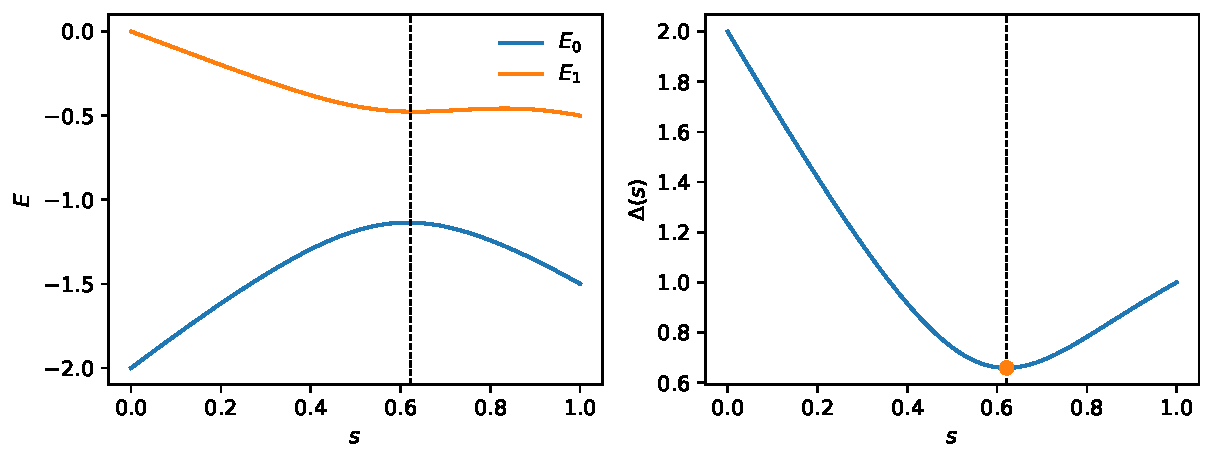
\includegraphics[width=0.95\textwidth]{figures/adi_ising_qiskit_gap.pdf}
	\caption{طیف لحظه‌ای و گاف مسیر همین مثال، بازتولیدشده با اسکریپت \lr{Qiskit}
		. کمینهٔ گاف $\Delta_{\min}\simeq0.65886$ نزدیک $s_*\simeq0.62$ است.}
	\label{fig:adi-ising-qiskit-gap}
\end{figure}

\paragraph{گام ج - برآورد زمان مؤثر $T$.}
با نرم طیفی
$\lVert H_P-H_B\rVert_2\simeq2.3696$
و خطای هدف $\varepsilon\sim10^{-2}$، تخمین مرتبه‌ای بخش قبل تکرار می‌شود:
\begin{equation}
	\label{eq:T-heur-qiskit}
	T_{\mathrm{heur}}
	\gtrsim
	\frac{\lVert H_P-H_B\rVert_2}{\Delta_{\min}^{2}\,\varepsilon}
	\simeq
	5.5\times10^{2}.
\end{equation}
این یک کران اکتشافی محافظه‌کارانه است، نه زمانِ کمینهٔ عملی. حل عددی معادلهٔ شرودینگر روی همین مسیر خطی نشان می‌دهد برای این سامانهٔ دوکیوبیتی، احتمال موفقیت $P(\lvert00\rangle)$ از حدود $T\simeq20$ به نزدیک یک می‌رسد و در $T=40$ عملاً اشباع می‌شود (جدول~\ref{tab:adi-T-success}). در مدار دیجیتال زیر از $T=40$ به‌عنوان زمان نمایشی استفاده می‌کنیم؛ اگر بخواهید با~\eqref{eq:T-heur-qiskit} هم‌تراز باشید، همان $T\sim500$ را با گام‌های تروترِ متناسب بگیرید.

\code{python}{snippets/adi_ising_03_runtime.py}{code:adi-ising-T}

\begin{table}[htbp]
	\centering
	\caption{احتمال ایده‌آلِ خوانش $\lvert00\rangle$ پس از تحول دقیقِ قطعه‌ای روی $H(s_k)$ (مرجع کلاسیک برای سنجش تروتر).}
	\label{tab:adi-T-success}
	\begin{tabular}{cccccc}
		\toprule
		$T$ & $5$ & $20$ & $40$ & $100$ & $500$ \\
		\midrule
		$P(\lvert00\rangle)$ & $0.74$ & $0.99$ & $\approx1$ & $\approx1$ & $\approx1$ \\
		\bottomrule
	\end{tabular}
\end{table}

\paragraph{گام د --- از $H(s)$ تا گیت‌ها (یک لایهٔ تروتر).}
در هر برش زمانیِ کوچک $\Delta t=T/N$ با $s$ ثابت،
\begin{equation}
	e^{-iH(s)\Delta t}
	\approx
	e^{i a X_0}\,
	e^{i a X_1}\,
	e^{i b Z_0Z_1}\,
	e^{i c Z_0}\,
	e^{i c Z_1},
\end{equation}
که
$a=(1-s)h_x\Delta t$،
$b=sJ\Delta t$،
$c=sh_z\Delta t$.
با قرارداد گیت‌های \lr{Qiskit}
($R_x(\theta)=e^{-i\theta X/2}$ و مشابه برای $R_z$ و $R_{zz}$) این یعنی
\begin{equation}
	R_x(-2a),\;
	R_{zz}(-2b),\;
	R_z(-2c).
\end{equation}
شکل~\ref{fig:adi-ising-trotter} اسکلت مدار را نشان می‌دهد: هادامارد برای $\lvert++\rangle$، سپس $N$ لایه با $s_k=(k+\tfrac12)/N$، و اندازه‌گیری در پایهٔ $Z$.

\code{python}{snippets/adi_ising_04_trotter_slice.py}{code:adi-ising-trotter}

\begin{figure}[htbp]
	\centering
	\begin{latin}
		\setstretch{1}
		\resizebox{\ifdim\width>\textwidth\textwidth\else\width\fi}{!}{%
			% Digital adiabatic: prep + one Trotter layer of H(s), then measure at the end
% سبک مشترک نمودارهای سند پایه‌ها (فقط داخل محیط latin فراخوانی شود)
\tikzset{
	qafbox/.style={
		draw=black!55,
		rounded corners=2pt,
		align=center,
		inner sep=3pt,
		thick,
		fill=white,
		font=\footnotesize\linespread{1}\selectfont,
		minimum height=0.95cm
	},
	qafwide/.style={
		qafbox,
		text width=2.55cm
	},
	qafnarr/.style={
		qafbox,
		text width=2.05cm
	},
	qaftitle/.style={
		font=\small\bfseries\linespread{1}\selectfont,
		align=center
	},
	qafarr/.style={
		-{Latex[length=2.2mm]},
		thick,
		draw=black!65
	},
	qafpanel/.style={
		draw,
		thick,
		rounded corners=4pt,
		inner xsep=8pt,
		inner ysep=8pt
	}
}

\begin{tikzpicture}[
	x=0.82cm,
	y=0.95cm,
	font=\footnotesize,
	note/.style={font=\scriptsize, text=black!55}
	]
	\draw[thick] (0,2) -- (10.8,2);
	\draw[thick] (0,0.6) -- (10.8,0.6);
	\node[left] at (0,2) {$q_0$};
	\node[left] at (0,0.6) {$q_1$};

	\node[qafbox, fill=blue!12, minimum width=0.65cm, minimum height=0.5cm] at (0.85,2) {$H$};
	\node[qafbox, fill=blue!12, minimum width=0.65cm, minimum height=0.5cm] at (0.85,0.6) {$H$};
	\node[note] at (0.85,2.55) {$\lvert++\rangle$};

	\draw[thick, densely dashed] (1.55,-0.05) rectangle (8.55,2.7);
	\node[note] at (5.05,3.0) {layer $k$: $s_k=(k+\tfrac12)/N$,\; $\Delta t=T/N$};

	\node[qafbox, fill=orange!14, minimum width=1.2cm, minimum height=0.5cm] at (2.55,2) {$R_x(-2a)$};
	\node[qafbox, fill=orange!14, minimum width=1.2cm, minimum height=0.5cm] at (2.55,0.6) {$R_x(-2a)$};

	\fill (4.2,2) circle (2.1pt);
	\fill (4.2,0.6) circle (2.1pt);
	\draw[thick] (4.2,2) -- (4.2,0.6);
	\node[qafbox, fill=green!12, minimum width=1.4cm, minimum height=0.48cm] at (5.35,1.3) {$R_{zz}(-2b)$};

	\node[qafbox, fill=cyan!12, minimum width=1.2cm, minimum height=0.5cm] at (7.15,2) {$R_z(-2c)$};
	\node[qafbox, fill=cyan!12, minimum width=1.2cm, minimum height=0.5cm] at (7.15,0.6) {$R_z(-2c)$};

	\node[qafbox, fill=gray!14, minimum width=0.8cm, minimum height=0.5cm] at (9.7,2) {$Z$};
	\node[qafbox, fill=gray!14, minimum width=0.8cm, minimum height=0.5cm] at (9.7,0.6) {$Z$};
	\node[note] at (9.7,2.55) {readout};

	\node[note, align=left] at (5.2,-0.75) {%
		$a=(1-s)h_x\Delta t$,\quad $b=sJ\Delta t$,\quad $c=sh_z\Delta t$};
\end{tikzpicture}
%
		}
	\end{latin}
	\caption{مدار آدیاباتیک دیجیتال برای مثال دوکیوبیتی: آماده‌سازی، لایه‌های تروترِ $H(s)$، خوانش $Z$.}
	\label{fig:adi-ising-trotter}
\end{figure}

\paragraph{گام ه - مدار کامل و خوانش.}
با $T=40$ و $N=200$ لایه، شبیه‌ساز حالت‌بردار تقریباً تمام وزن احتمال را روی $\lvert00\rangle$ می‌گذارد
($P(\lvert00\rangle)\simeq0.9999$ در اجرای
\lr{qcomputing}؛
در \lr{AerSimulator} با $4096$ شات همهٔ شمارش‌ها $\mathtt{00}$ بودند).
همین اجرا شکل~\ref{fig:adi-ising-qiskit-gap} را نیز می‌نویسد.

\code{python}{snippets/adi_ising_05_run.py}{code:adi-ising-run}

\paragraph{جمع‌بندی عملی.}
\begin{enumerate}
	\item $H_B$ و $H_P$ را به‌صورت \lr{SparsePauliOp} بنویسید؛ $H(s)$ همان ترکیب خطی است.
	\item با قطری‌سازی روی شبکهٔ $s$، $\Delta_{\min}$ و $s_*$ را استخراج کنید (اینجا $\simeq0.66$ در $s\simeq0.62$).
	\item $T_{\mathrm{heur}}$ را از~\eqref{eq:T-heur-qiskit} برآورد کنید؛ برای این مثال کوچک $T\sim40$ هم در تحول دقیق و تروتر کافی است.
	\item مسیر را با تروترِ مرتبهٔ اول به گیت‌های $R_x$/$R_{zz}$/$R_z$ بشکنید و در پایان در پایهٔ $Z$ بخوانید.
\end{enumerate}
برای بازتولید اعداد بدون نصب \lr{Qiskit} می‌توانید
\lr{figures/adi\_ising\_qiskit\_verify.py}
را اجرا کنید. بخش بعد گاف را از زاویهٔ پژوهشی باز می‌کند؛ ورودی عددی‌اش همین مسیر است.

% BEGIN GAP RESEARCH EXPANSION
\begingroup
\emergencystretch=2em


%========================
%========================
\section{گاف انرژی: تعریف دقیق و نقش تقارن}
\label{sec:gap-research}

گاف انرژی یکی از کمیت‌های اصلی در تحلیل شبیه‌سازی ادیاباتیک است، اما
تفسیر آن باید متناسب با ساختار طیف و فضای حالت موردنظر انجام شود.
فرض کنید هامیلتونی وابسته به پارامتر بی‌بُعد $s\in[0,1]$ به صورت
$H(s)$ تعریف شده باشد و مقادیر ویژه و بردارهای ویژه‌ی آن از رابطه‌ی
\begin{equation}
	H(s)|j(s)\rangle = E_j(s)|j(s)\rangle,
	\qquad
	E_0(s)\leq E_1(s)\leq E_2(s)\leq\cdots
\end{equation}
به دست آیند. در شبیه‌سازی ادیاباتیک، پارامتر $s$ معمولاً تابعی از زمان
است، یعنی $s=s(t)$، و سامانه از هامیلتونی اولیه $H(0)$ به هامیلتونی
نهایی $H(1)$ منتقل می‌شود.

در ساده‌ترین حالت، که حالت پایه در تمام مسیر یکتا باشد، گاف انرژی
به صورت فاصله‌ی میان حالت پایه و نخستین حالت برانگیخته تعریف می‌شود:
\begin{equation}
	\Delta(s)=E_1(s)-E_0(s).
	\label{eq:ground-state-gap}
\end{equation}
با این حال، این تعریف در همه‌ی مسائل کافی نیست. ممکن است چند تراز
پایین انرژی به صورت یک زیر‌فضای هدف در نظر گرفته شوند، یا تقارن
هامیلتونی باعث شود برخی ترازها از نظر دینامیکی برای حالت اولیه
قابل‌دسترسی نباشند. از این رو، تحلیل گاف در این بخش در سه مرحله انجام
می‌شود: نخست، شناسایی ترازهای مرتبط در یک مقدار ثابت از $s$؛ دوم،
یافتن کمینه‌ی گاف در سراسر مسیر $0\leq s\leq1$؛ و سوم، بررسی رفتار
این کمینه با افزایش اندازه‌ی سامانه. در نهایت، گاف باید در کنار
عناصر ماتریسی گذار و سرعت تغییر $s$ تفسیر شود، زیرا کوچک‌ترین فاصله‌ی
انرژی به تنهایی تعیین‌کننده‌ی احتمال گذار غیرادیاباتیک نیست.

برای فرمول‌های این بخش $\hbar$ به‌صورت صریح نوشته می‌شود. در
محاسبات عددی، انرژی‌ها بر حسب واحد $J$ و زمان‌ها بر حسب
$\hbar/J$ بیان شده‌اند.

\subsection{گاف کل، گاف بخش تقارنی و گاف زیر‌فضای هدف}
\label{subsec:gap-types}

اگر حالت پایه یکتا باشد، کمیت طبیعی برای سنجش جدایی حالت پایه از
نخستین حالت برانگیخته همان گاف رابطه‌ی
\eqref{eq:ground-state-gap} است. در این حالت، کوچک شدن
$\Delta(s)$ به معنای نزدیک شدن دو تراز پایین انرژی است و معمولاً
شرایط ادیاباتیک را دشوارتر می‌کند. با این حال، در بسیاری از مسائل
ممکن است چند حالت پایین انرژی به طور همزمان بخشی از فضای هدف را
تشکیل دهند. در این حالت، مهم‌ترین کمیت الزاماً شکافت میان ترازهای
داخل این زیر‌فضا نیست، بلکه فاصله‌ی این زیر‌فضا از نخستین تراز
خارج از آن است.

فرض کنید $q$ تراز پایین انرژی، یعنی
\[
|0(s)\rangle,\ldots,|q-1(s)\rangle,
\]
زیر‌فضای هدف را تشکیل دهند. پروژکتور روی این زیر‌فضا به صورت
\begin{equation}
	P(s)
	=
	\sum_{j=0}^{q-1}
	|j(s)\rangle\langle j(s)|
	\label{eq:target-projector}
\end{equation}
تعریف می‌شود. نخستین تراز خارج از این زیر‌فضا، تراز شماره‌ی $q$ است؛
بنابراین گاف میان آخرین تراز داخل زیر‌فضا و نخستین تراز خارج از آن
به صورت
\begin{equation}
	g_{\mathrm{out}}(s)
	=
	E_q(s)-E_{q-1}(s)
	\label{eq:subspace-gap}
\end{equation}
تعریف می‌شود.

این تعریف یک تفاوت مفهومی مهم با گاف معمول حالت پایه دارد. برای
مثال، اگر $q=2$ باشد، فضای هدف توسط دو حالت
$|0(s)\rangle$ و $|1(s)\rangle$ تشکیل می‌شود و
\begin{equation}
	P(s)
	=
	|0(s)\rangle\langle0(s)|
	+
	|1(s)\rangle\langle1(s)|.
\end{equation}
در این حالت ممکن است فاصله‌ی
\[
E_1(s)-E_0(s)
\]
بسیار کوچک باشد، اما اگر فاصله‌ی
\[
E_2(s)-E_1(s)
\]
بزرگ باقی بماند، سامانه همچنان می‌تواند در زیر‌فضای دوبعدی هدف
باقی بماند. بنابراین کوچک بودن شکافت درون یک خوشه از ترازها، به
خودی خود به معنای خروج سامانه از آن زیر‌فضا نیست.

در چنین حالتی، معیار طبیعی موفقیت در پایان فرآیند، احتمال قرار گرفتن
حالت نهایی در زیر‌فضای هدف است:
\begin{equation}
	P_{\mathrm{succ}}
	=
	\langle\Psi(T)|P(1)|\Psi(T)\rangle.
	\label{eq:success-probability}
\end{equation}
اگر $q=1$ باشد، رابطه‌ی فوق به احتمال حضور در حالت پایه‌ی نهایی
کاهش می‌یابد:
\begin{equation}
	P_{\mathrm{succ}}
	=
	|\langle0(1)|\Psi(T)\rangle|^2.
\end{equation}
اما برای $q>1$، حالت نهایی لازم نیست با یک بردار ویژه‌ی منفرد
منطبق باشد و کافی است در زیر‌فضای هدف قرار داشته باشد.

\subsubsection{نقش تقارن در تعریف گاف مرتبط}

یکی دیگر از مواردی که می‌تواند تفسیر گاف را تغییر دهد، وجود یک
تقارن پایسته در طول مسیر است. فرض کنید $S$ اپراتور تقارن هامیلتونی
باشد و در تمام مسیر داشته باشیم
\begin{equation}
	[H(s),S]=0.
	\label{eq:symmetry-commutation}
\end{equation}
اگر $S$ مستقل از $s$ باشد، با مشتق‌گیری از رابطه‌ی
\eqref{eq:symmetry-commutation} نسبت به $s$ نیز نتیجه می‌شود که
\begin{equation}
	[\partial_s H(s),S]=0.
	\label{eq:derivative-symmetry}
\end{equation}

در نتیجه، فضای هیلبرت را می‌توان به بخش‌های تقارنی مستقل
(\lr{symmetry sectors}) تجزیه کرد. به طور نمادین می‌توان نوشت
\begin{equation}
	\mathcal{H}
	=
	\bigoplus_{\alpha}\mathcal{H}_{\alpha},
\end{equation}
که در آن هر $\mathcal{H}_{\alpha}$ با یک مقدار یا نمایش مشخص از
تقارن $S$ متناظر است. اگر حالت اولیه در یکی از این بخش‌ها قرار
داشته باشد و تقارن در تمام مسیر دقیقاً حفظ شود، دینامیک ایده‌آل
سامانه در همان بخش باقی می‌ماند.

%%==============
%===============
اگر دو حالت $|a\rangle$ و $|b\rangle$ به دو \lr{sector} متفاوت از تقارن
متعلق باشند،
\[S|a\rangle=s_{\alpha}|a\rangle,
\qquad
S|b\rangle=s_{\beta}|b\rangle,
\qquad
s_{\alpha}\neq s_{\beta},\]
از شرط $[H(s),S]=0$ می‌توان یک قانون انتخاب برای عناصر ماتریسی
هامیلتونی به دست آورد. از رابطه‌ی
\[H(s)S=S H(s)\]
و ضرب از چپ در $\langle b|$ و از راست در $|a\rangle$ داریم
\[s_{\alpha}\langle b|H(s)|a\rangle
=
s_{\beta}\langle b|H(s)|a\rangle.\]
بنابراین
\begin{equation}
	(s_{\alpha}-s_{\beta})
	\langle b|H(s)|a\rangle=0,
\end{equation}
و در نتیجه، برای $s_{\alpha}\neq s_{\beta}$،
\begin{equation}
	\langle b|H(s)|a\rangle=0.
	\label{eq:symmetry-selection-rule-H}
\end{equation}


%===============
%===============

این موضوع باعث می‌شود کوچک‌ترین گاف در کل طیف همیشه گاف مرتبط با
دینامیک سامانه نباشد. برای مثال، ممکن است دو تراز متعلق به دو بخش
تقارنی متفاوت باشند و در یک نقطه‌ی $s=s^\ast$ به یکدیگر برسند:
\begin{equation}
	E_a(s^\ast)=E_b(s^\ast),
	\qquad
	|a\rangle\in\mathcal{H}_{\alpha},
	\quad
	|b\rangle\in\mathcal{H}_{\beta},
	\quad
	\alpha\neq\beta.
\end{equation}
در این حالت، گاف کل طیف می‌تواند در $s^\ast$ صفر شود، در حالی که
انتقال میان دو حالت به دلیل تقارن مجاز نیست. به بیان دیگر، صفر شدن
گاف کل الزاماً به معنای وقوع یک گذار غیرادیاباتیک میان دو حالت
نیست.

از این رو، اگر حالت اولیه در یک sector مشخص قرار داشته باشد، علاوه
بر گاف کل، باید گاف در بخش تقارنی قابل‌دسترسی نیز بررسی شود. اگر
$E_{0,\alpha}(s)$ و $E_{1,\alpha}(s)$ به ترتیب پایین‌ترین و
نزدیک‌ترین تراز بالاتر در sector $\alpha$ باشند، می‌توان نوشت
\begin{equation}
	\Delta_{\alpha}(s)
	=
	E_{1,\alpha}(s)-E_{0,\alpha}(s).
	\label{eq:sector-gap}
\end{equation}
در نتیجه، در یک سیستم با تقارن دقیق، مقایسه‌ی
$g_{\min}^{\mathrm{global}}$ با
$g_{\min}^{\mathrm{sector}}$ می‌تواند نشان دهد که آیا کوچک‌ترین
گاف مشاهده‌شده در کل طیف واقعاً برای دینامیک موردنظر قابل‌دسترسی
است یا ناشی از برخورد ترازهای بخش‌های مختلف تقارنی است.

برای دینامیک ادیاباتیک، عنصر ماتریسی مرتبط با تحریک ناشی از تغییر
پارامتر $s$، یعنی
$\langle b|\partial_s H|a\rangle$، اهمیت مستقیم‌تری دارد. از آنجا که
$S$ مستقل از $s$ است و
\[[H(s),S]=0,\]
داریم
\[[\partial_s H(s),S]=0.\]
بنابراین همان قانون انتخاب برای مشتق هامیلتونی نیز برقرار است:
\begin{equation}
	\langle b|\partial_s H(s)|a\rangle=0,
	\qquad
	s_{\alpha}\neq s_{\beta}.
	\label{eq:symmetry-selection-rule-dH}
\end{equation}
با استفاده از رابطه‌ی
\[\langle b|\partial_s a\rangle
=
\frac{
	\langle b|\partial_sH|a\rangle
}{
	E_a-E_b},\]
نتیجه می‌شود که
\begin{equation}
	\langle b|\partial_s a\rangle=0.
	\label{eq:symmetry-no-transition}
\end{equation}
از این رو، در صورت حفظ دقیق تقارن، تغییر ادیاباتیک هامیلتونی نمی‌تواند
به طور مستقیم حالتی را از یک \lr{sector} به \lr{sector} دیگر منتقل کند.


این حفاظت، البته، به حفظ تقارن وابسته است. اگر نویز یا یک اغتشاش
اضافی $H_{\mathrm{noise}}$ تقارن را بشکند، به طوری که
\begin{equation}
	[H_{\mathrm{noise}},S]\neq0,
\end{equation}
آنگاه \lr{sector} های مختلف دیگر کاملاً مستقل نیستند و انتقال میان آنها می‌تواند مجاز شود. بنابراین در تحلیل‌های واقع‌گرایانه، گاف بخش
تقارنی و گاف کل باید در کنار اثرات شکست تقارن ناشی از نویز تفسیر
شوند.

در نتیجه، ممکن است دو تراز متعلق به \lr{sector} های متفاوت در نقطه‌ای
$s=s^\ast$ یکدیگر را قطع کنند:
\begin{equation}
	E_a(s^\ast)=E_b(s^\ast),
	\qquad
	a\in\mathcal H_{\alpha},
	\quad
	b\in\mathcal H_{\beta},
	\quad
	\alpha\neq\beta.
\end{equation}
در این حالت، گاف کل طیف می‌تواند صفر شود، اما به دلیل رابطه‌ی
\eqref{eq:symmetry-selection-rule-dH} عنصر ماتریسی مسئول این گذار
صفر است. بنابراین این \lr{crossing} لزوماً یک کانال گذار قابل‌دسترسی
برای سامانه ایجاد نمی‌کند.

\subsubsection{تفاوت گاف‌های فیزیکی مختلف}

اصطلاح «گاف انرژی» در زمینه‌های مختلف فیزیک به کمیت‌های متفاوتی
اشاره می‌کند و این کمیت‌ها الزاماً با یکدیگر برابر نیستند. برای
مثال، در سامانه‌ای با تعداد ذرات $N$، گاف مرتبط با تغییر تعداد ذرات
ممکن است به صورت
\begin{equation}
	\Delta_{\mathrm{charge}}
	=
	E_0(N+1)+E_0(N-1)-2E_0(N)
	\label{eq:charge-gap}
\end{equation}
تعریف شود. این کمیت با گاف میان ترازهای یک هامیلتونی بس‌ذره‌ای در
تعداد ذرات ثابت یکسان نیست. همچنین گاف تک‌ذره‌ای و گاف اپتیکی
می‌توانند به دلیل تفاوت در فرآیندهای فیزیکی و قواعد انتخاب، مقادیر
متفاوتی داشته باشند.

در این فصل، منظور از گاف، مگر آنکه خلاف آن تصریح شود، گاف کم‌انرژی
هامیلتونی بس‌ذره‌ای در مسیر مشخص $H(s)$ است. بنابراین نخستین
قله یا گذار قابل‌اندازه‌گیری در یک مشاهده‌پذیر تجربی الزاماً با
کوچک‌ترین گاف طیفی یکسان نیست؛ قواعد انتخاب و عناصر ماتریسی
مشاهده‌پذیر می‌توانند برخی گذارها را سرکوب یا برخی دیگر را تقویت
کنند.

\subsection{چرا کوچک‌ترین فاصله به‌تنهایی کافی نیست؟}
\label{subsec:gap-not-sufficient}

اگرچه کوچک‌ترین گاف یکی از مهم‌ترین کمیت‌های مورد استفاده در
تحلیل ادیاباتیک است، اما به تنهایی مشخص نمی‌کند که کدام حالت
بر‌انگیخته بیشترین احتمال گذار را دارد. برای مشاهده‌ی این موضوع،
معادله‌ی مقدار ویژه‌ی حالت پایه را در نظر می‌گیریم:
\begin{equation}
	H(s)|0(s)\rangle
	=
	E_0(s)|0(s)\rangle.
	\label{eq:ground-state-eigenvalue}
\end{equation}
با مشتق‌گیری نسبت به $s$ داریم
\begin{equation}
	\partial_s H\,|0\rangle
	+
	H\,|\partial_s0\rangle
	=
	(\partial_sE_0)|0\rangle
	+
	E_0|\partial_s0\rangle.
\end{equation}
اکنون دو طرف را از چپ در $\langle m(s)|$ ضرب می‌کنیم. با استفاده
از رابطه‌ی
\[
\langle m|H=E_m\langle m|
\]
و متعامد بودن حالت‌های ویژه برای $m\neq0$،
\[
\langle m|0\rangle=0,
\]
به دست می‌آوریم
\begin{equation}
	\langle m|\partial_sH|0\rangle
	+
	E_m\langle m|\partial_s0\rangle
	=
	E_0\langle m|\partial_s0\rangle.
\end{equation}
در نتیجه،
\begin{equation}
	\langle m|\partial_s0\rangle
	=
	-\frac{\langle m|\partial_sH|0\rangle}
	{E_m-E_0}
	=
	\frac{\langle m|\partial_sH|0\rangle}
	{E_0-E_m},
	\qquad m>0.
	\label{eq:gap-eigenvector-derivative}
\end{equation}

این رابطه نشان می‌دهد که حساسیت حالت پایه به تغییر پارامتر $s$
صرفاً به فاصله‌ی انرژی وابسته نیست. صورت کسر،
\[
\langle m|\partial_sH|0\rangle,
\]
نشان‌دهنده‌ی شدت کوپل شدن حالت پایه با حالت $m$ در اثر تغییر
هامیلتونی است، در حالی که مخرج با فاصله‌ی انرژی میان دو حالت تعیین
می‌شود.

برای جدا کردن این دو اثر، تعریف می‌کنیم
\begin{equation}
	\Delta_{m0}(s)
	=
	E_m(s)-E_0(s),
	\qquad
	M_{m0}(s)
	=
	\left|
	\langle m(s)|\partial_sH(s)|0(s)\rangle
	\right|.
	\label{eq:gap-and-matrix-element}
\end{equation}
بنابراین رابطه‌ی \eqref{eq:gap-eigenvector-derivative} از نظر
اندازه به صورت
\begin{equation}
	\left|
	\langle m|\partial_s0\rangle
	\right|
	=
	\frac{M_{m0}}{\Delta_{m0}}
	\label{eq:eigenvector-sensitivity}
\end{equation}
درمی‌آید.

اکنون باید توجه داشت که $s$ تابع زمان است. بنابراین
\begin{equation}
	\frac{d}{dt}|0(s(t))\rangle
	=
	\dot{s}(t)\,\partial_s|0(s(t))\rangle.
	\label{eq:time-dependent-ground-state}
\end{equation}
در نتیجه، هرچه سرعت تغییر $s$ بیشتر باشد، تغییر لحظه‌ای بردار حالت
نیز بیشتر خواهد بود. ترکیب سرعت تغییر پارامتر، عنصر ماتریسی گذار و
فاصله‌ی انرژی، شاخص بی‌بُعد محلی زیر را به دست می‌دهد:
\begin{equation}
	a_m(t)
	=
	\frac{
		\hbar|\dot{s}(t)|\,M_{m0}(s(t))
	}{
		\Delta_{m0}(s(t))^2
	}.
	\label{eq:gap-local-indicator}
\end{equation}
کوچک بودن $a_m(t)$ نشان‌دهنده‌ی قرار داشتن فرآیند در ناحیه‌ای است
که در آن انتظار می‌رود کوپل دینامیکی میان حالت پایه و حالت $m$
ضعیف باشد. با این حال، $a_m$ یک شاخص محلی است و کوچک بودن آن به
تنهایی جایگزین یک قضیه‌ی دقیق ادیاباتیک یا حل مستقیم معادله‌ی
شرودینگر نمی‌شود.

رابطه‌ی \eqref{eq:gap-local-indicator} همچنین روشن می‌کند که چرا
نزدیک‌ترین تراز انرژی الزاماً مهم‌ترین کانال گذار نیست. اگر برای
یک حالت نزدیک داشته باشیم
\begin{equation}
	\Delta_{m0}\ll\Delta_{n0},
	\qquad
	M_{m0}=0,
\end{equation}
آن حالت از این کانال مستقیماً تحریک نمی‌شود و سهم متناظر در
شاخص $a_m$ صفر است. در مقابل، یک حالت دورتر ممکن است دارای عنصر
ماتریسی بزرگی باشد و در نتیجه شاخص بزرگ‌تری داشته باشد:
\begin{equation}
	\frac{M_{n0}}{\Delta_{n0}^2}
	>
	\frac{M_{m0}}{\Delta_{m0}^2}.
\end{equation}
بنابراین، تحلیل دقیق مسیر ادیاباتیک باید دست‌کم سه کمیت را در کنار
یکدیگر بررسی کند: فاصله‌ی انرژی $\Delta_{m0}$، عنصر ماتریسی
$M_{m0}$، و سرعت تغییر $|\dot{s}|$.

در نتیجه، کمینه‌ی گاف انرژی همچنان یک شاخص بنیادی برای تشخیص نقاط
حساس مسیر است، اما برای تفسیر دینامیک باید مشخص شود که این گاف
میان کدام ترازهاست، آیا ترازهای موردنظر در یک بخش تقارنی یکسان
قرار دارند، و عنصر ماتریسی اتصال آنها به حالت اولیه چقدر است.
این تفکیک میان «نزدیکی طیفی» و «قابل‌دسترسی بودن دینامیکی» مبنای
تحلیل زمان‌بندی ادیاباتیک در ادامه‌ی این فصل خواهد بود.



%=========================
%=========================
%

\section{از گاف تا زمان: شرط محلی، کران و آزمون دینامیکی}
\label{sec:gap-runtime}

گاف انرژی به‌تنهایی یک کمیت طیفی است، در حالی که در شبیه‌سازی
ادیاباتیک پرسش اصلی این است که سامانه با چه سرعتی می‌تواند در طول
مسیر $H(s)$ حرکت کند، بدون آنکه از فضای هدف خارج شود. بنابراین برای
تبدیل اطلاعات گاف به یک زمان اجرا، باید علاوه بر فاصله انرژی، نرخ
تغییر هامیلتونی و کوپلینگ میان حالت‌های لحظه‌ای را نیز در نظر گرفت.
اگر

$$
H(s)|j(s)\rangle=E_j(s)|j(s)\rangle,
\qquad
s=s(t),
\qquad
s(0)=0,\quad s(T)=1,
$$

باشد، آنگاه $T$ زمان کل اجرای فرایند است. در حالت ایده‌آل ادیاباتیک،
هرچه تغییر هامیلتونی آهسته‌تر باشد، احتمال باقی‌ماندن در فضای هدف
بیشتر خواهد بود. با این حال، «زمان لازم» را می‌توان به چند معنای
متفاوت تعریف کرد و این تعاریف الزاماً به یک مقدار یکسان منتهی
نمی‌شوند.

\subsection{سه معنای متفاوت برای زمان لازم}

نخستین مفهوم، \textit{زمان مقیاسی} است. در بسیاری از بیان‌های ساده
قضیه ادیاباتیک، زمان اجرا به‌صورت کیفی با معکوس توان دوم گاف کمینه
مقیاس می‌شود:
\begin{equation}
	T_{\mathrm{scale}}
	\sim
	\frac{\hbar}{g_{\min}^{,2}},
	\qquad
	g_{\min}=\min_{0\leq s\leq1}g(s).
	\label{eq:adiabatic-scale}
\end{equation}
این رابطه برای فهم وابستگی کیفی مفید است: اگر گاف کمینه کاهش یابد،
معمولاً باید زمان بیشتری برای تکامل اختصاص داد. برای مثال، کاهش گاف
به نصف، در این تخمین ساده می‌تواند مقیاس زمانی را تا حدود چهار برابر
افزایش دهد. با این حال، رابطه~\eqref{eq:adiabatic-scale} یک قانون
دقیق برای زمان اجرای هر مسئله نیست، زیرا نرخ تغییر هامیلتونی و
عناصر ماتریسی میان حالت‌ها نیز در تحریک نقش دارند.

مفهوم دوم، \textit{کران کافی} است. در این حالت هدف این نیست که زمان
واقعی موردنیاز را پیش‌بینی کنیم، بلکه می‌خواهیم شرطی به دست آوریم
که اگر برقرار باشد، خطای ادیاباتیک از مقدار مشخصی بزرگ‌تر نشود.
قضایای دقیق ادیاباتیک، تحت فرض‌هایی مانند همواری مسیر و وجود گاف
مثبت، چنین کران‌هایی را فراهم می‌کنند. این کران‌ها معمولاً
محافظه‌کارانه‌اند و ممکن است زمانی بزرگ‌تر از زمان موردنیاز واقعی
ارائه دهند.

مفهوم سوم، \textit{زمان عملی} است. در اینجا تکامل واقعی سامانه برای
زمان‌های مختلف $T$ محاسبه یا اندازه‌گیری می‌شود و سپس زمان موردنیاز
بر اساس یک معیار موفقیت تعیین می‌گردد. برای مثال، اگر $P(1)$
پروژکتور فضای هدف در انتهای مسیر باشد، می‌توان نوشت
\begin{equation}
	P_{\mathrm{succ}}(T)=
	\langle\Psi(T)|P(1)|\Psi(T)\rangle.
	\label{eq:success-vs-time}
\end{equation}
اگر آستانه موفقیت موردنظر $P_{\mathrm{target}}$ باشد، یک تعریف
عملی از زمان لازم می‌تواند کوچک‌ترین $T$ای باشد که
\begin{equation}
	P_{\mathrm{succ}}(T)\geq P_{\mathrm{target}}.
	\label{eq:practical-runtime}
\end{equation}
بنابراین باید میان سه کمیت تمایز گذاشت:
\begin{equation}
	T_{\mathrm{scale}},
	\qquad
	T_{\mathrm{bound}},
	\qquad
	T_{\mathrm{practical}}.
\end{equation}
این سه کمیت معمولاً یکسان نیستند؛ اولی یک مقیاس کیفی، دومی یک
کران نظری و سومی نتیجه مستقیم دینامیک یا آزمایش است.

\subsection{از شرط محلی تا کران ادیاباتیک}

برای درک وابستگی زمان به گاف، ابتدا از معادله ویژه لحظه‌ای شروع
می‌کنیم:
\begin{equation}
	H(s)|0(s)\rangle=E_0(s)|0(s)\rangle.
\end{equation}
با مشتق‌گیری نسبت به $s$ و در نظر گرفتن یک حالت ویژه
$|m(s)\rangle$ با $m>0$، در حالت غیرتبهگن داریم
\begin{equation}
	\langle m|\partial_s0\rangle =
	\frac{\langle m|\partial_sH|0\rangle}
	{E_0-E_m}.
	\label{eq:runtime-eigenstate-derivative}
\end{equation}
اگر
\begin{equation}
	\Delta_{m0}(s)=E_m(s)-E_0(s),
	\qquad
	M_{m0}(s)=
	\left|
	\langle m(s)|\partial_sH(s)|0(s)\rangle
	\right|,
\end{equation}
تعریف کنیم، آنگاه
\begin{equation}
	\left|\langle m|\partial_s0\rangle\right|=
	\frac{M_{m0}(s)}{\Delta_{m0}(s)}.
	\label{eq:eigenstate-sensitivity}
\end{equation}

از طرف دیگر، چون $s=s(t)$ است،
\begin{equation}
	\frac{d}{dt}|0(s(t))\rangle=
	\dot{s}(t) \partial_s|0(s)\rangle.
\end{equation}
در نتیجه، هرچه $|\dot{s}|$ بزرگ‌تر باشد، حالت لحظه‌ای با سرعت
بیشتری در فضای هیلبرت حرکت می‌کند. از ترکیب این رابطه با ساختار
دینامیک ادیاباتیک، یک شاخص محلی از نوع
\begin{equation}
	a_m(t)=
	\frac{
		\hbar |\dot{s}(t)|,M_{m0}(s)
	}{
		\Delta_{m0}(s)^2
	}
	\label{eq:runtime-local-indicator}
\end{equation}
به دست می‌آید. کوچک بودن این کمیت برای همه کانال‌های مهم، نشانه‌ای
از حرکت آهسته در آن ناحیه است. با این حال، $a_m$ یک شاخص محلی است
و به‌تنهایی یک قضیه کامل درباره احتمال خطای نهایی ارائه نمی‌کند.

این رابطه سه عامل را به‌صورت همزمان نشان می‌دهد:
\begin{equation}
	\boxed{
		\text{حساسیت ادیاباتیک}
		\sim
		\frac{
			\text{سرعت تغییر مسیر}\times
			\text{کوپلینگ}
		}{
			\text{گاف}^2
		}
	}.
\end{equation}
بنابراین کوچک بودن گاف به‌تنهایی تعیین‌کننده نیست. یک تراز نزدیک
اگر

$$
M_{m0}\approx0
$$

باشد، ممکن است کانال مؤثری برای تحریک ایجاد نکند؛ در مقابل، یک تراز
دورتر با عنصر ماتریسی بزرگ می‌تواند سهم مهم‌تری در خطا داشته باشد.

\subsection{کران‌های سراسری برای خطای ادیاباتیک}

یک قضیه دقیق‌تر باید رفتار کل مسیر را در نظر بگیرد، نه فقط مقدار
گاف در یک نقطه. برای یک پایه یکتا، مسیر دوبار مشتق‌پذیر و وجود یک
گاف مثبت در سراسر مسیر، ساختار یک کران از نوع
\lr{Jansen--Ruskai--Seiler} برای دامنه نشت را می‌توان به‌صورت
\begin{align}
	\epsilon_{\mathrm{amp}}(T)
	&\leq
	\frac{C\hbar}{T}
	\left[
	\frac{|H'(0)|}{g(0)^2}
	+
	\frac{|H'(1)|}{g(1)^2}
	%	\right.
	%	&\left.
	+\int_0^1
	\left(
	\frac{|H''(s)|}{g(s)^2}
	+
	\frac{|H'(s)|^2}{g(s)^3}
	\right)ds
	\right].
	\label{eq:gap-rigorous-structure}
\end{align}
در این رابطه، $C$ یک ثابت عددی مستقل از $T$ است و نمایش فوق برای
نشان‌دادن ساختار وابستگی‌ها نوشته شده است، نه به‌عنوان نقل دقیق
ثابت‌های بهینه یک قضیه خاص. کمیت $g(s)$ فاصله فضای هدف از بخش
قابل‌دسترسی خارج از آن را نشان می‌دهد؛ برای یک پایه یکتا معمولاً
می‌توان آن را به‌صورت

$$
g(s)=E_1(s)-E_0(s)
$$

در نظر گرفت.

ساختار رابطه~\eqref{eq:gap-rigorous-structure} چند نکته مهم را
روشن می‌کند. نخست، گاف تنها کمیتی نیست که زمان را تعیین می‌کند:
مشتق اول هامیلتونی، یعنی $H'(s)$، نرخ تغییر مسیر را مشخص می‌کند و
مشتق دوم، یعنی $H''(s)$، اطلاعاتی درباره تغییر این نرخ در طول مسیر
وارد می‌کند. دوم، وابستگی به گاف شدید است؛ جمله‌هایی با
$1/g(s)^2$ و $1/g(s)^3$ نشان می‌دهند که نواحی با گاف کوچک می‌توانند
سهم بزرگی در کران خطا داشته باشند. سوم، کران به کل مسیر وابسته است
و نه فقط به نقطه‌ای که $g(s)$ کمینه می‌شود.

در اینجا باید میان دامنه خطا و احتمال خطا نیز تمایز گذاشت. اگر
حالت نهایی به‌صورت
\begin{equation}
	|\Psi(T)\rangle=
	a_0|0(1)\rangle
	+
	\sum_{m>0}a_m|m(1)\rangle
\end{equation}
نوشته شود، آنگاه احتمال نشت از حالت هدف برابر است با
\begin{equation}
	P_{\mathrm{leak}}=	
	\sum_{m>0}|a_m|^2.
\end{equation}
در مقابل، یک کران روی اندازه دامنه مؤلفه خارج از فضای هدف را می‌توان
با کمیتی مانند $\epsilon_{\mathrm{amp}}$ بیان کرد. بنابراین در
ساختار ساده
\begin{equation}
	P_{\mathrm{leak}}
	\sim
	\epsilon_{\mathrm{amp}}^2.
	\label{eq:amplitude-probability}
\end{equation}
در نتیجه اگر یک قضیه کرانی از نوع
$\epsilon_{\mathrm{amp}}\leq A/T$ ارائه دهد، نباید همان کمیت را
مستقیماً «احتمال خطا» نامید. این تمایز به‌ویژه هنگام مقایسه کران
نظری با نتایج عددی یا تجربی اهمیت دارد~\cite{GapJansen2007}.

\subsection{زمان‌بندی محلی: کجا باید آهسته‌تر رفت؟}

کران‌های سراسری برای تضمین رفتار ادیاباتیک مفیدند، اما برای طراحی
یک زمان‌بندی مناسب می‌توان از اطلاعات محلی نیز استفاده کرد. با
توجه به شاخص~\eqref{eq:runtime-local-indicator}، تعریف می‌کنیم
\begin{equation}
	K(s)=
	\max_{m>0}
	\frac{M_{m0}(s)}
	{\Delta_{m0}(s)^2}.
	\label{eq:local-sensitivity-K}
\end{equation}
این کمیت بزرگ‌ترین حساسیت محلی را در میان کانال‌های تحریک از حالت
هدف به ترازهای دیگر نشان می‌دهد.

اگر $K(s)$ در بخشی از مسیر بزرگ باشد، بهتر است سامانه در آن ناحیه
آهسته‌تر حرکت کند. یک زمان‌بندی اکتشافی از این ایده به‌صورت
\begin{equation}
	\frac{dt}{ds}=	
	\frac{\hbar}{\eta}
	\max{K(s),K_{\mathrm{floor}}}
	\label{eq:gap-local-schedule}
\end{equation}
تعریف می‌شود. در اینجا $\eta$ یک پارامتر کنترل‌کننده سرعت و
$K_{\mathrm{floor}}>0$ یک کف عددی برای جلوگیری از سرعت‌های نامحدود
است. با انتگرال‌گیری، زمان کل متناظر با این زمان‌بندی برابر است با
\begin{equation}
	T_{\mathrm{loc}}=
	\frac{\hbar}{\eta}
	\int_0^1
	\max{K(s),K_{\mathrm{floor}}} ds.
	\label{eq:local-runtime}
\end{equation}

رابطه~\eqref{eq:gap-local-schedule} را می‌توان به‌صورت فیزیکی چنین
تفسیر کرد:
\begin{equation}
	K(s)\uparrow
	\quad\Longrightarrow\quad
	\frac{dt}{ds}\uparrow
	\quad\Longrightarrow\quad
	\text{حرکت آهسته‌تر},
\end{equation}
در حالی که
\begin{equation}
	K(s)\downarrow
	\quad\Longrightarrow\quad
	\frac{dt}{ds}\downarrow
	\quad\Longrightarrow\quad
	\text{حرکت سریع‌تر}.
\end{equation}
بنابراین زمان به‌صورت یکنواخت در کل مسیر توزیع نمی‌شود، بلکه در
نواحی حساس‌تر زمان بیشتری صرف می‌شود.

وجود $K_{\mathrm{floor}}$ نیز از این جهت ضروری است که اگر $K(s)$
در ناحیه‌ای بسیار کوچک یا صفر شود، رابطه بدون کف می‌توانست مقدار
$dt/ds$ بسیار کوچکی ایجاد کند و در نتیجه سرعت

$$
\dot{s}=\frac{ds}{dt}
$$

به مقادیر غیرواقعی بزرگی برسد. در یک پیاده‌سازی عملی، علاوه بر این
کف، محدودیت‌های کنترل مانند
\begin{equation}
	|\dot{s}(t)|\leq v_{\max},
	\qquad
	|\ddot{s}(t)|\leq a_{\max}
\end{equation}
نیز باید در نظر گرفته شوند.

نکته مهم دیگر آن است که $K(s)$ الزاماً در همان نقطه‌ای بیشینه
نمی‌شود که گاف کمینه است. زیرا
\begin{equation}
	K(s)=
	\max_m
	\frac{M_{m0}(s)}{\Delta_{m0}(s)^2}
\end{equation}
هم‌زمان به گاف و عنصر ماتریسی وابسته است. بنابراین در حالت کلی
\begin{equation}
	\arg\min_s\Delta(s)
	\neq
	\arg\max_sK(s).
\end{equation}
این نتیجه نشان می‌دهد که طراحی زمان‌بندی فقط با یافتن کوچک‌ترین
گاف انجام نمی‌شود و باید کوپلینگ میان حالت‌ها نیز بررسی شود.

پارامتر $\eta$ در رابطه~\eqref{eq:gap-local-schedule} صرفاً یک
پارامتر طراحی برای کنترل سرعت است. بنابراین به‌طور کلی نمی‌توان
نوشت

$$
P_{\mathrm{error}}=\eta
\qquad\text{یا}\qquad
P_{\mathrm{error}}=\eta^2.
$$

برای تبدیل $\eta$ به یک تضمین کمی درباره احتمال خطای نهایی، به
تحلیل مستقل و دقیق‌تری نیاز است. از این رو، زمان‌بندی محلی باید
به‌عنوان یک روش طراحی و اکتشاف در نظر گرفته شود، نه یک تضمین
خودکار برای احتمال موفقیت.

برای مقایسه، اگر زمان‌بندی خطی انتخاب شود،
\begin{equation}
	s(t)=\frac{t}{T},
	\qquad
	\dot{s}=\frac{1}{T},
\end{equation}
سرعت در تمام مسیر ثابت است. در چنین حالتی، یک مقیاس محلی ساده
برای زمان از مرتبه
\begin{equation}
	T_{\mathrm{lin}}
	\sim
	\frac{\hbar}{\eta}\max_s K(s)
\end{equation}
به دست می‌آید. زمان‌بندی غیرخطی با استفاده از~\eqref{eq:local-runtime}
به‌جای یک سرعت ثابت، زمان بیشتری را به نواحی حساس اختصاص می‌دهد.

نتایج \lr{Roland--Cerf} در مسئله ساختاریافته جست‌وجوی کوانتومی
نمونه‌ای از این ایده هستند: انتخاب زمان‌بندی محلی مناسب می‌تواند
در آن مسئله نسبت به زمان‌بندی یکنواخت بهبود مقیاسی ایجاد کند.
با این حال، این نتیجه به ساختار ویژه آن مسئله وابسته است و نباید
به‌عنوان تضمینی عمومی برای هر هامیلتونی از نوع آیزینگ یا هر مسیر
ادیاباتیک دیگر تفسیر شود~\cite{GapRoland2002}.

\subsection{تفاوت مسیر هامیلتونی و زمان‌بندی}

دو مفهوم «مسیر» و «زمان‌بندی» باید از یکدیگر تفکیک شوند. اگر
هامیلتونی به‌صورت

$$
H=H(s)
$$

ثابت باشد و تنها تابع $s(t)$ تغییر کند، نقاطی که در فضای هامیلتونی
طی می‌شوند تغییر نمی‌کنند. در نتیجه طیف

$$
E_j(s)
$$

و منحنی گاف

$$
g(s)
$$

همان باقی می‌مانند؛ تنها سرعت عبور از این منحنی تغییر می‌کند.

در مقابل، اگر خود مسیر تغییر کند،
\begin{equation}
	H_1(s)\neq H_2(s),
\end{equation}
آنگاه به‌طور کلی
\begin{equation}
	E_j^{(1)}(s)\neq E_j^{(2)}(s),
	\qquad
	g_1(s)\neq g_2(s).
\end{equation}
بنابراین می‌توان میان دو نوع طراحی تمایز گذاشت:
\begin{equation}
	\boxed{
		\text{زمان‌بندی}
		\longrightarrow
		\text{نحوه عبور از یک مسیر ثابت}
	}
\end{equation}
و
\begin{equation}
	\boxed{
		\text{طراحی مسیر}
		\longrightarrow
		\text{تغییر خود طیف و گاف}.
	}
\end{equation}
این تمایز در بهینه‌سازی ادیاباتیک اهمیت اساسی دارد، زیرا افزایش
زمان همیشه تنها راه بهبود عملکرد نیست؛ در برخی مسائل می‌توان با
تغییر مسیر $H(s)$، گاف را نیز تغییر داد.

\subsection{تقاطع اجتنابی و تقریب دو‌ترازی}

یکی از مهم‌ترین موقعیت‌هایی که رابطه میان گاف و زمان را به‌صورت
شفاف نشان می‌دهد، ناحیه نزدیک یک تقاطع اجتنابی است. فرض کنید دو
تراز بدون کوپل‌شدن، یعنی ترازهای دیاباتیک، در نزدیکی
$t=t_*$ به هم نزدیک شوند. یک مدل مؤثر دو‌ترازی برای این ناحیه را
می‌توان به‌صورت
\begin{equation}
	H_{\mathrm{eff}}(t)=
	\frac{v(t-t_*)}{2}\sigma_z
	+
	\frac{g}{2}\sigma_x
	\label{eq:landau-zener-hamiltonian}
\end{equation}
نوشت. در نمایش ماتریسی،
\begin{equation}
	H_{\mathrm{eff}}(t)=
	\frac{1}{2}
	\begin{pmatrix}
		v(t-t_*)&g\
		g&-v(t-t_*)
	\end{pmatrix}.
\end{equation}

اگر $g=0$ باشد، دو تراز دیاباتیک

$$
E_a(t)=\frac{v(t-t_*)}{2},
\qquad
E_b(t)=-\frac{v(t-t_*)}{2}
$$

در $t=t_*$ یکدیگر را قطع می‌کنند. وجود جمله

$$
\frac{g}{2}\sigma_x
$$

بین دو حالت coupling ایجاد می‌کند و این crossing را به یک
\lr{avoided crossing} تبدیل می‌کند. مقادیر ویژه هامیلتونی
~\eqref{eq:landau-zener-hamiltonian} برابرند با
\begin{equation}
	E_\pm(t)=	
	\pm\frac{1}{2}
	\sqrt{v^2(t-t_*)^2+g^2},
\end{equation}
و بنابراین فاصله دو تراز برابر است با
\begin{equation}
	\Delta(t)
	=
	E_+(t)-E_-(t)
	=
	\sqrt{v^2(t-t_*)^2+g^2}.
	\label{eq:landau-zener-gap}
\end{equation}
در نقطه $t=t_*$ داریم
\begin{equation}
	\Delta_{\min}=g.
\end{equation}
در این قرارداد، $g$ مستقیماً برابر با گاف کمینه است.

پارامتر $v$ نیز سرعت تغییر اختلاف انرژی ترازهای دیاباتیک را
مشخص می‌کند. زیرا در نبود coupling،
\begin{equation}
	E_a(t)-E_b(t)=v(t-t_*),
\end{equation}
و در نتیجه
\begin{equation}
	v=
	\frac{d}{dt}
	\left(E_a-E_b\right).
\end{equation}
بنابراین $g$ اندازه گاف کمینه و $|v|$ سرعت جاروب در ناحیه
تقاطع را مشخص می‌کند.

برای جاروب خطی ایده‌آل از $t=-\infty$ تا $t=+\infty$، فرمول
\lr{Landau--Zener} احتمال گذار غیرادیااباتیک را به‌صورت
\begin{equation}
	P_{\mathrm{exc}}=	
	\exp\left[
	-\frac{\pi g^2}
	{2\hbar|v|}
	\right]
	\label{eq:landau-zener-probability}
\end{equation}
می‌دهد. این رابطه به‌وضوح نشان می‌دهد که افزایش گاف کمینه،
احتمال تحریک را کاهش می‌دهد:
\begin{equation}
	g\uparrow
	\quad\Longrightarrow\quad
	P_{\mathrm{exc}}\downarrow,
\end{equation}
در حالی که جاروب سریع‌تر احتمال تحریک را افزایش می‌دهد:
\begin{equation}
	|v|\uparrow
	\quad\Longrightarrow\quad
	P_{\mathrm{exc}}\uparrow.
\end{equation}
در حد جاروب بسیار آهسته،

$$
|v|\rightarrow0,
$$

داریم

$$
P_{\mathrm{exc}}\rightarrow0.
$$

رابطه~\eqref{eq:landau-zener-probability} همچنین نشان می‌دهد که
فقط مقدار گاف کمینه مهم نیست، بلکه سرعت عبور از ناحیه حساس نیز
اهمیت دارد. برای مثال، از رابطه~\eqref{eq:landau-zener-gap} می‌توان
دید که مقیاس پهنای زمانی ناحیه‌ای که گاف در نزدیکی مقدار کمینه خود
باقی می‌ماند، با
\begin{equation}
	\Delta t_{\mathrm{sens}}
	\sim
	\frac{g}{|v|}
\end{equation}
مقیاس می‌شود. بنابراین یک تقاطع با گاف کوچک، اما عبور بسیار آهسته،
می‌تواند رفتاری متفاوت از تقاطعی با همان گاف و جاروب بسیار سریع
داشته باشد.

با این حال، رابطه لاندائو--زنر شرایط مشخصی دارد: تقریب دو‌ترازی،
جاروب خطی، مسیر زمانی نامحدود از منفی بی‌نهایت تا مثبت بی‌نهایت و
نبود اثرات محیطی. در یک مسیر محدود، در حضور چند تقاطع، یا در یک
سامانه باز و اتلافی، رابطه~\eqref{eq:landau-zener-probability}
لزوماً یک نتیجه دقیق نیست و باید به‌عنوان یک مدل یا تقریب محلی
استفاده شود~\cite{AlbashLidar2018}.

\subsection{از کران نظری تا آزمون دینامیکی}

در نهایت، هیچ‌یک از مقیاس‌های ساده، کران‌های نظری یا زمان‌بندی‌های
محلی جایگزین بررسی مستقیم دینامیک نمی‌شوند. برای یک زمان‌بندی
مشخص $s(t)$، حالت واقعی سامانه از معادله شرودینگر به دست می‌آید:
\begin{equation}
	i\hbar\frac{d}{dt}|\Psi(t)\rangle=
	H(s(t))|\Psi(t)\rangle,
	\qquad
	|\Psi(0)\rangle=|\Psi_0\rangle.
	\label{eq:time-dependent-schrodinger}
\end{equation}
در انتهای فرایند،

$$
s(T)=1,
$$

و بنابراین حالت

$$
|\Psi(T)\rangle
$$

حالت واقعی تولیدشده توسط دینامیک است، نه لزوماً حالت ویژه نهایی.
برای یک حالت پایه یکتا، اگر تکامل کاملاً ادیاباتیک باشد، انتظار
می‌رود
\begin{equation}
	|\Psi(T)\rangle
	\approx
	e^{i\gamma}
	|0(1)\rangle,
\end{equation}
که در آن $\gamma$ فاز کلی است. در حالت کلی‌تر، اگر هدف یک زیر‌فضای
چندبعدی باشد، معیار مناسب همان احتمال قرارگیری در پروژکتور هدف است:
\begin{equation}
	P_{\mathrm{succ}}(T)=	
	\langle\Psi(T)|P(1)|\Psi(T)\rangle.
\end{equation}

بنابراین یک روش عملی برای ارزیابی زمان اجرا آن است که برای چند
مقدار $T$ تکامل زمانی حل شود و تابع

$$
P_{\mathrm{succ}}(T)
$$

به‌دست آید. سپس می‌توان زمان عملی را با یک آستانه مشخص مانند

$$
P_{\mathrm{succ}}\geq0.99
$$

تعریف کرد. این آزمون دینامیکی می‌تواند نشان دهد که آیا کران نظری
بیش از حد محافظه‌کارانه بوده است، آیا زمان‌بندی محلی واقعاً مفید
بوده است، و آیا کانال‌های تحریک پیش‌بینی‌شده از تحلیل گاف در عمل
مهم هستند یا خیر.

در نتیجه، ارتباط میان گاف و زمان را نباید به یک فرمول منفرد مانند
$T\propto1/g_{\min}^2$ تقلیل داد. ساختار کامل‌تر را می‌توان به‌صورت
زنجیره زیر خلاصه کرد:
\begin{equation}
	H(s)
	\longrightarrow
	{E_j(s)}
	\longrightarrow
	g(s)
	\longrightarrow
	M_{m0}(s)
	\longrightarrow
	K(s)
	\longrightarrow
	s(t)
	\longrightarrow
	|\Psi(T)\rangle
	\longrightarrow
	P_{\mathrm{succ}}(T).
\end{equation}
در این زنجیره، گاف اطلاعات طیفی را فراهم می‌کند، عناصر ماتریسی
نشان می‌دهند کدام حالت‌ها واقعاً با تغییر هامیلتونی کوپل می‌شوند،
زمان‌بندی سرعت عبور از مسیر را تعیین می‌کند و در نهایت حل مستقیم
دینامیک مشخص می‌کند که زمان انتخاب‌شده واقعاً به موفقیت موردنظر
منجر شده است.




\section{مقیاس‌پذیری با اندازهٔ سیستم}
\label{sec:complexity-scaling}

بخش~\ref{sec:gap-runtime} زمان لازم را برای \emph{یک} مسیر $H(s)$ با $n$ ثابت می‌سنجد.
اینجا همان پرسش را برای یک \emph{خانواده} از مسیرها مطرح می‌کنیم: وقتی سامانه بزرگ می‌شود، $\Delta_{\min}$ و $T$ چگونه رشد می‌کنند؟
این همان تعمیمی است که در پایان مثال دوکیوبیتی (بخش~\ref{sec:adi-ising-example}، روابط~\eqref{eq:HB-n}--\eqref{eq:H-n-interpolation}) باز شد.
جزئیات حل‌پذیر زنجیرهٔ \lr{TFIM}، شکل عددی گاف، و ارتباط با \lr{QMA} در بخش~\ref{sec:gap-scaling} می‌آید.

در بررسی پیچیدگی یک الگوریتم آدیاباتیک معمولاً یک سامانهٔ منفرد را بررسی نمی‌کنیم، بلکه خانواده‌ای از سامانه‌ها را در نظر می‌گیریم که با افزایش یک پارامتر اندازه بزرگ‌تر می‌شوند. این پارامتر را با $n$ نشان می‌دهیم. برای بسیاری از مدل‌های اسپینی، $n$ همان تعداد اسپین یا کیوبیت است. در حالت کلی تعریف اندازه به ساختار مدل بستگی دارد: در یک زنجیره $n$ طول زنجیره است و در شبکهٔ $d$بعدی با طول خطی $L$
\begin{equation}
	n\sim L^d.
\end{equation}

بنابراین منظور از «اندازهٔ سیستم» صرفاً یک عدد مربوط به تعداد کیوبیت‌ها نیست؛ بلکه پارامتری است که با افزایش آن، خانواده‌ای از مسائل بزرگ‌تر تعریف می‌شود. برای مثال، می‌توان خانواده‌ای از هامیلتونی‌ها را به صورت
\begin{equation}
	H_n(s)
\end{equation}
تعریف کرد و سپس برای هر مقدار $n$، گاف کمینهٔ مسیر را محاسبه نمود:
\begin{equation}
	\Delta_{\min}(n)=
	\min_{0\leq s\leq1}\Delta_n(s).
	\label{eq:gap-min-system-size}
\end{equation}

\subsection{چرا تعداد کیوبیت به‌تنهایی معیار دشواری نیست؟}

برای یک سامانهٔ $n$ کیوبیتی، بعد فضای هیلبرت برابر است با
\begin{equation}
	D=2^n.
\end{equation}
بنابراین با افزایش $n$، فضای حالت به‌صورت نمایی بزرگ می‌شود. با این حال، در یک مسئلهٔ ادیاباتیک، دشواری حل مسئله را نمی‌توان صرفاً از روی $2^n$ تعیین کرد. یکی از مهم‌ترین کمیت‌های تعیین‌کننده، گاف انرژی در طول مسیر است:
\begin{equation}
	\Delta_{\min}(n).
\end{equation}

به بیان دیگر، دو مسئله با تعداد یکسانی کیوبیت می‌توانند از نظر ادیاباتیک دشواری کاملاً متفاوتی داشته باشند. بنابراین زنجیره اصلی برای تحلیل مقیاس‌پذیری را می‌توان به‌صورت زیر نوشت:
\begin{equation}
	\boxed{
		n
		\longrightarrow
		H_n(s)
		\longrightarrow
		\Delta_{\min}(n)
		\longrightarrow
		T(n)
		\longrightarrow
		\text{پیچیدگی}
	}
\end{equation}

در این زنجیره $n$ اندازهٔ مسئله را مشخص می‌کند، $H_n(s)$ خانواده را تعریف می‌کند، $\Delta_{\min}(n)$ رفتار گاف را می‌دهد و همان رفتار زمان آدیاباتیک را می‌سازد.

\paragraph{سه خانواده مرتبط با مثال‌های همین فصل.}
برای اینکه $n$ مجرد نماند، همان زبان میدان عرضی / \lr{Ising} را نگه می‌داریم:
\begin{enumerate}
	\item \textbf{فقط هامیلتونی آغازین.}
	$H_n=-h_x\sum_{i=1}^{n}X_i$ همان $H_B$ در~\eqref{eq:HB-n} است.
	گاف برای هر $n$ برابر $2h_x$ می‌ماند؛ بزرگ کردن سامانه فضا را بزرگ می‌کند ولی گلوگاه آدیاباتیک را عوض نمی‌کند.
	\item \textbf{زنجیرهٔ \lr{TFIM}.}
	ادامهٔ طبیعی مثال دوکیوبیتی به $n$ سایت با جفت‌شدگی نزدیک‌ترین همسایه:
	\begin{equation}
		H_n(s)
		=
		-(1-s)h_x\sum_i X_i
		-
		s\Bigl(J\sum_{i=1}^{n-1}Z_iZ_{i+1}+h_z\sum_i Z_i\Bigr).
	\end{equation}
	عضو $n=2$ با $h_z=1/4$ همان بخش~\ref{sec:adi-ising-example} است.
	اگر $h_z=0$ و مسیر به نقطهٔ بحرانی $h_x/J=1$ برسد، گاف کل مثل $1/n$ بسته می‌شود (بخش~\ref{sec:gap-scaling}).
	\item \textbf{شکافت نمایی.}
	در فاز مرتبِ همان زنجیره باز، یا در مسیرهایی با تونل‌زنی میان دو چاه، شکافت دو تراز کم‌انرژی می‌تواند مثل $e^{-cn}$ جمع شود؛ گاف حجمی تحریک‌ها ممکن است محدود بماند.
\end{enumerate}

\subsection{بسته‌شدن چندجمله‌ای گاف}

یکی از حالت‌های متداول این است که گاف کمینه با افزایش اندازه سیستم به‌صورت توانی کاهش یابد:
\begin{equation}
	\Delta_{\min}(n)
	\sim
	n^{-\alpha},
	\qquad
	\alpha>0.
	\label{eq:polynomial-gap-closing}
\end{equation}

در این رابطه، $\alpha$ یک \textit{نمای مقیاس} است. این عدد مشخص می‌کند گاف با چه توانی از اندازه سیستم کاهش پیدا می‌کند. برای مثال، اگر
$\alpha=1$
آنگاه
\begin{equation}
	\Delta_{\min}(n)\sim\frac{1}{n}.
\end{equation}
اگر
$\alpha=2 $
داشته باشیم،
\begin{equation}
	\Delta_{\min}(n)\sim\frac{1}{n^2}.
\end{equation}
بنابراین هرچه $\alpha$ بزرگ‌تر باشد، در این مقیاس‌بندی گاف سریع‌تر با افزایش $n$ کوچک می‌شود.

نمونه‌ای از همین رفتار، زنجیره باز \lr{TFIM} در نقطه بحرانی $g=h/J=1$ است.
گاف دقیق (همان~\eqref{eq:gap-open-chain} در بخش~\ref{sec:gap-scaling}) برای $n$ بزرگ
\begin{equation}
	\Delta_{\min}(n)
	\simeq
	\frac{\pi J}{n}
	\label{eq:tfim-critical-gap}
\end{equation}
می‌شود؛ پس $\alpha=1$. پیش‌عامل $\pi J$ مقیاس انرژی محلی را حمل می‌کند.

در اینجا $J$ یک مقیاس انرژی است و ضریب $\pi J$ پیش‌عامل مقیاس‌بندی را تعیین می‌کند. نکته مهم این است که $\alpha$ یک پارامتر جهانی و مستقل از مدل نیست؛ مقدار آن از فیزیک سامانه و
نحوه بسته‌شدن گاف ناشی می‌شود.

در نزدیکی یک گذار فاز کوانتومی پیوسته، این رفتار را گاهی به شکل عمومی‌تری می‌توان نوشت:
\begin{equation}
	\Delta_{\min}
	\sim
	L^{-z},
\end{equation}
که در آن $L$ طول خطی سیستم و $z$ \textit{نمای دینامیکی} است. اگر اندازه سیستم با تعداد درجات آزادی رابطه
$n\sim L^d$ داشته باشد، آنگاه
\begin{equation}
	L\sim n^{1/d}
\end{equation}
و در نتیجه
\begin{equation}
	\Delta_{\min}
	\sim
	n^{-z/d}.
\end{equation}
بنابراین در چنین حالتی می‌توان
$\alpha=\frac{z}{d}$
را به‌عنوان نمای مقیاس نسبت به $n$ در نظر گرفت.

\subsection{بسته‌شدن نمایی گاف}

رفتار مهم دیگری که ممکن است رخ دهد، بسته‌شدن نمایی گاف است:
\begin{equation}
	\Delta_{\min}(n)
	\sim
	e^{-cn},
	\qquad
	c>0.
	\label{eq:exponential-gap-closing}
\end{equation}

در اینجا $c$ یک \textit{نرخ بسته‌شدن نمایی} است. برخلاف $\alpha$ که یک توان بدون‌بُعد در مقیاس‌بندی توانی است، واحد $c$ به نحوه تعریف اندازه سیستم بستگی دارد. اگر $n$ یک عدد بدون‌بُعد مانند تعداد کیوبیت باشد، $c$ نیز بدون‌بُعد است.

برای مثال، اگر
$c=0.1$
آنگاه گاف تقریباً مانند $e^{-0.1n}$ کاهش می‌یابد. اگر $c$ بزرگ‌تر باشد، گاف با افزایش $n$ سریع‌تر بسته می‌شود.

بسته‌شدن نمایی گاف معمولاً نشانه وجود یک فرآیند فیزیکی بسیار ضعیف در مقیاس بزرگ است. برای مثال، در برخی مسائل ممکن است دو حالت کم‌انرژی با یک سد مؤثر از یکدیگر جدا باشند و جفت‌شدگی مؤثر میان آنها با افزایش اندازه سیستم به‌صورت نمایی کاهش یابد. در چنین شرایطی شکافت دو تراز می‌تواند رفتاری مانند
\begin{equation}
	\Delta_{\min}\sim e^{-cn}
\end{equation}
پیدا کند.

در این حالت، مقدار $c$ به جزئیات مدل وابسته است و می‌تواند تحت تأثیر عواملی مانند قدرت برهم‌کنش‌ها، شکل سد مؤثر، شرایط مرزی، تقارن و نوع مسیر هامیلتونی قرار گیرد. بنابراین $c$ نیز مانند
$\alpha$ یک ثابت جهانی نیست.

\subsection{چگونه بسته‌شدن گاف به زمان اجرا منتقل می‌شود؟}

اکنون ارتباط میان مقیاس گاف و زمان ادیاباتیک را می‌توان روشن‌تر دید. در یک تخمین ساده ادیاباتیک، زمان اجرا به‌صورت
\begin{equation}
	T
	\sim
	\frac{\hbar}{\Delta_{\min}^{2}}
	\label{eq:runtime-gap-scaling}
\end{equation}
مقیاس می‌شود. این همان تخمین مقیاسی بخش‌های~\ref{sec:adiabatic-theorem} و~\ref{sec:gap-runtime} است، نه یک کران کافیِ عمومی.

اگر گاف به‌صورت چندجمله‌ای بسته شود،
\begin{equation}
	\Delta_{\min}(n)
	\sim
	n^{-\alpha},
\end{equation}
با قرار دادن آن در~\eqref{eq:runtime-gap-scaling} داریم
\begin{align}
	T(n)
	&\sim
	\frac{\hbar}
	{\bigl(n^{-\alpha}\bigr)^2}
	\sim
	\hbar\, n^{2\alpha}.
\end{align}
بنابراین، با صرف‌نظر از ثابت‌های انرژی و ضرایب مستقل از $n$،
\begin{equation}
	\boxed{
		T(n)\sim n^{2\alpha}
	}
\end{equation}
به دست می‌آید. در نتیجه اگر $\alpha$ ثابت باشد، زمان اجرا همچنان با اندازه سیستم به‌صورت چندجمله‌ای رشد می‌کند.

برای مثال، اگر

$$
\Delta_{\min}\sim\frac{1}{n},
$$

آنگاه
$
T\sim n^2
$
.

اما اگر گاف به‌صورت نمایی بسته شود،
\begin{equation}
	\Delta_{\min}(n)
	\sim
	e^{-cn},
\end{equation}
خواهیم داشت
\begin{align}
	T(n)
	&\sim
	\frac{\hbar}
	{\bigl(e^{-cn}\bigr)^2}
	\sim
	\hbar\, e^{2cn}.
\end{align}
بنابراین
\begin{equation}
	\boxed{
		T(n)\sim e^{2cn}
	}
\end{equation}
خواهد بود که رشد نمایی دارد.

این نتیجه اهمیت زیادی دارد: ممکن است یک الگوریتم ادیاباتیک برای اندازه‌های کوچک کاملاً قابل‌اجرا باشد، اما اگر گاف آن با اندازه سیستم به‌صورت نمایی بسته شود، زمان لازم برای حفظ رفتار ادیاباتیک می‌تواند با افزایش $n$ به‌سرعت غیرعملی شود.

\subsection{ضرایب و معنای آنها}

در روابط مقیاس‌بندی، باید میان \textit{نمای مقیاس} و
\textit{پیش‌عامل} تفاوت گذاشت. برای مثال، رابطه
\begin{equation}
	\Delta_{\min}(n)
	\sim
	A n^{-\alpha}
\end{equation}
دارای دو نوع پارامتر است:

\begin{itemize}
	\item $\alpha$ نمای مقیاس است و مشخص می‌کند گاف با چه توانی از
	$n$ کاهش می‌یابد؛
	
	\item $A$ پیش‌عامل است و مقیاس انرژی مسئله و جزئیات مدل را
	تعیین می‌کند.
	
\end{itemize}

به‌طور مشابه، برای بسته‌شدن نمایی می‌توان نوشت
\begin{equation}
	\Delta_{\min}(n)
	\sim
	A e^{-cn},
\end{equation}
که در آن $A$ پیش‌عامل انرژی و $c$ نرخ بسته‌شدن نمایی است.

اگر $n$ تعداد کیوبیت باشد، $n$ بدون‌بُعد است و $c$ نیز بدون‌بُعد خواهد بود. اگر اندازهٔ سیستم با یک کمیت دارای واحد، مانند طول $L$، تعریف شود، آنگاه $c$ واحد معکوس همان کمیت را خواهد داشت.

پیش‌عامل $A$ معمولاً برای تعیین رفتار مجانبی مهم نیست، زیرا در مقیاس‌بندی با $n$ ثابت است؛ اما برای محاسبهٔ زمان واقعی و مقایسه سامانه‌ها در اندازه‌های محدود می‌تواند اهمیت زیادی داشته باشد.

\subsection{تعداد کیوبیت و دشواری مسئله}

از این بحث روشن می‌شود که تعداد کیوبیت به‌تنهایی معیار مناسبی برای دشواری یک مسئله آدیاباتیک نیست. سه خانوادهٔ بالا را می‌توان در یک جدول جمع کرد:

\begin{table}[htbp]
	\centering
	\small
	\setstretch{1.15}
	\caption{سه رژیم نوعی برای خانوادهٔ $H_n(s)$. زمان‌ها تخمین مقیاسی $T\sim\hbar/\Delta_{\min}^{2}$اند، نه کران قضیه.}
	\label{tab:scaling-regimes}
	\begin{tabularx}{\textwidth}{@{}
			>{\raggedright\arraybackslash}p{4.4cm}
			>{\raggedright\arraybackslash}X
			>{\raggedright\arraybackslash}p{3.6cm}
			@{}}
		\toprule
		\rowcolor{gray!14}
		\textbf{خانواده} & \textbf{گاف} & \textbf{زمان نوعی} \\
		\midrule
		فقط هامیلتونی آغازین: $H=-h_x\sum_i X_i$
		& $\Delta_{\min}=2h_x$ (مستقل از $n$)
		& $T$ مستقل از $n$
		\\
		\rowcolor{gray!8}
		\lr{TFIM} بحرانی، زنجیره باز
		& $\Delta_{\min}\simeq\pi J/n$ \quad($\alpha=1$)
		& $T\sim n^{2}$
		\\
		تونل‌زنی / شکافت فاز مرتب
		& $\Delta_{\min}\sim e^{-cn}$
		& $T\sim e^{2cn}$
		\\
		\bottomrule
	\end{tabularx}
\end{table}

برای شهود عددی، سه منحنی را از همان $n=2$ مثال کاری بهنجار می‌کنیم:
$T(n)/T(2)$.
خانوادهٔ فقط‌هامیلتونی‌آغازین نسبت $1$ می‌ماند؛ رژیم $\alpha=1$ مثل $(n/2)^{2}$ رشد می‌کند؛ رژیم نمایی با $c=0.12$ مثل $e^{0.24(n-2)}$ رشد می‌کند.
شکل~\ref{fig:complexity-scaling} نشان می‌دهد که تا $n\simeq8$ دو رژیم متغیر هنوز نزدیک‌اند، ولی در $n=32$ شاخهٔ نمایی چند مرتبه بزرگ‌تر است.

\begin{figure}[htbp]
	\centering
	\begin{latin}
		\setstretch{1}
		\resizebox{0.92\textwidth}{!}{%
			% مقایسه شهودی سه رژیم: گاف ثابت، بسته شدن 1/n، بسته شدن نمایی
% نرمال شده به n=2 با Delta=0.66 (مثال دوکیوبیتی) برای دو رژیم متغیر
% سبک مشترک نمودارهای سند پایه‌ها (فقط داخل محیط latin فراخوانی شود)
\tikzset{
	qafbox/.style={
		draw=black!55,
		rounded corners=2pt,
		align=center,
		inner sep=3pt,
		thick,
		fill=white,
		font=\footnotesize\linespread{1}\selectfont,
		minimum height=0.95cm
	},
	qafwide/.style={
		qafbox,
		text width=2.55cm
	},
	qafnarr/.style={
		qafbox,
		text width=2.05cm
	},
	qaftitle/.style={
		font=\small\bfseries\linespread{1}\selectfont,
		align=center
	},
	qafarr/.style={
		-{Latex[length=2.2mm]},
		thick,
		draw=black!65
	},
	qafpanel/.style={
		draw,
		thick,
		rounded corners=4pt,
		inner xsep=8pt,
		inner ysep=8pt
	}
}

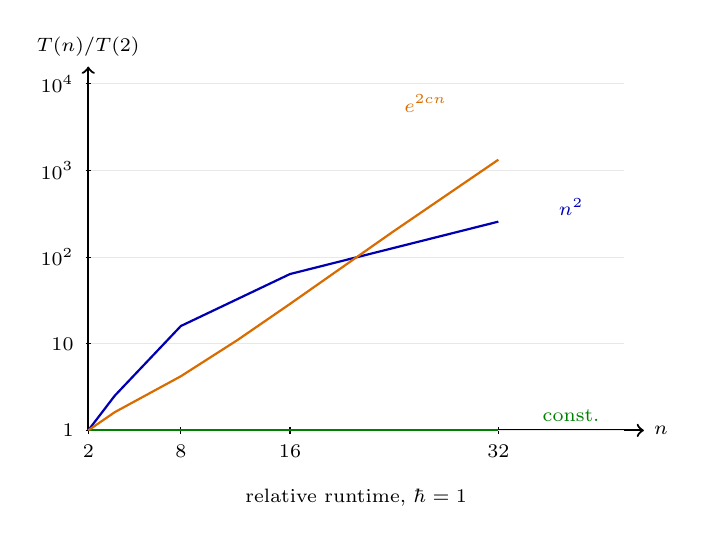
\begin{tikzpicture}[
	x=0.42cm,
	y=0.55cm,
	font=\scriptsize
	]
	% --- left: relative runtime T(n)/T(2) ---
	\draw[->, thick] (0,0) -- (16.8,0) node[right] {$n$};
	\draw[->, thick] (0,0) -- (0,8.4) node[above] {$T(n)/T(2)$};
	\foreach \x/\lab in {0/2, 2.8/8, 6.1/16, 12.4/32} {
		\draw (\x,0.08) -- (\x,-0.08);
		\node[below] at (\x,-0.12) {$\lab$};
	}
	\foreach \y/\lab in {0/1, 2/10, 4/10^{2}, 6/10^{3}, 8/10^{4}} {
		\draw[gray!18] (0,\y) -- (16.2,\y);
		\draw (-0.08,\y) -- (0.08,\y);
		\node[left] at (-0.15,\y) {$\lab$};
	}

	% Independent: T/T2 = 1  (log10 = 0)
	\draw[thick, green!50!black]
		(0,0) -- (12.4,0);
	\node[green!50!black] at (14.6,0.35) {const.};

	% Polynomial alpha=1: T/T2 = (n/2)^2
	% n=2,8,16,32 -> 1, 16, 64, 256
	% y = 2*log10(Trel) so 1->0, 16->2.4, 64->3.61, 256->4.82
	\draw[thick, blue!70!black]
		plot coordinates {
			(0.00,0.00)
			(0.80,0.80)
			(2.80,2.41)
			(6.10,3.61)
			(12.40,4.82)
		};
	\node[blue!70!black] at (14.6,5.15) {$n^{2}$};

	% Exponential c=0.12: T/T2 = exp(0.24(n-2))
	% n=2,8,16,24,32 -> 1, 4.22, 28.8, 196, 1339
	% y=2 log10: 0, 1.25, 2.92, 4.58, 6.25
	\draw[thick, orange!85!black]
		plot coordinates {
			(0.00,0.00)
			(0.80,0.42)
			(2.80,1.25)
			(4.50,2.08)
			(6.10,2.92)
			(9.20,4.58)
			(12.40,6.25)
		};
	\node[orange!85!black] at (10.2,7.55) {$e^{2cn}$};

	\node at (8.1,-1.55) {relative runtime, $\hbar=1$};
\end{tikzpicture}
%
		}
	\end{latin}
	\caption{زمان نسبی $T(n)/T(2)$ روی مقیاس لگاریتمی.
		سبز: گاف ثابت (فقط $H_B$).
		آبی: بسته‌شدن $1/n$ و $T\sim n^{2}$.
		نارنجی: $c=0.12$ و $T\sim e^{2cn}$.
		این شکل طرحوارهٔ مقیاس است، نه دادهٔ یک شبیه‌سازی خاص.}
	\label{fig:complexity-scaling}
\end{figure}

\begin{table}[htbp]
	\centering
	\small
	\caption{مقادیر $T(n)/T(2)$ برای همان سه رژیم شکل~\ref{fig:complexity-scaling}.}
	\label{tab:scaling-numbers}
	\begin{tabular}{cccc}
		\toprule
		\rowcolor{gray!14}
		$n$ & ثابت & $\alpha=1$ & $c=0.12$ \\
		\midrule
		$2$ & $1$ & $1$ & $1$ \\
		\rowcolor{gray!8}
		$8$ & $1$ & $16$ & $\simeq4.2$ \\
		$16$ & $1$ & $64$ & $\simeq29$ \\
		\rowcolor{gray!8}
		$32$ & $1$ & $256$ & $\simeq1.3\times10^{3}$ \\
		\bottomrule
	\end{tabular}
\end{table}

بنابراین دو سامانه با $n=32$ کیوبیت می‌توانند یکی زمانِ چندصد برابر $T(2)$ و دیگری هزار برابر داشته باشند.
معیار مناسب، رفتار خانواده و گاف آن است نه خودِ $n$.

پس معیار مناسب‌تر برای تحلیل پیچیدگی، بررسی رفتار خانواده هامیلتونی‌ها و گاف آن‌ها با افزایش اندازه سیستم است:
\begin{equation}
	H_n(s)
	\quad\longrightarrow\quad
	\Delta_{\min}(n)
	\quad\longrightarrow\quad
	T(n).
\end{equation}

\subsection{یک نکته مهم درباره مقیاس انرژی}

در مقایسه گاف‌ها و زمان‌های اجرا، باید مقیاس انرژی مسئله را نیز ثابت نگه داشت. اگر کل هامیلتونی را در یک ضریب ثابت $\lambda$ ضرب کنیم،
\begin{equation}
	H(s)\rightarrow\lambda H(s),
\end{equation}
تمام انرژی‌ها و در نتیجه گاف‌ها نیز به همان نسبت تغییر می‌کنند:
\begin{equation}
	\Delta(s)\rightarrow\lambda\Delta(s).
\end{equation}
از آنجا که مقیاس زمانی طبیعی کوانتومی با $\hbar/\Delta$ مرتبط است، افزایش کل مقیاس انرژی می‌تواند زمان فیزیکی را کاهش دهد. با این حال، این تغییر به‌تنهایی به معنای کاهش پیچیدگی محاسباتی مسئله نیست؛ زیرا در واقع مقیاس انرژی یا واحد زمان فیزیکی را تغییر داده‌ایم.

بنابراین هنگام مطالعه مقیاس‌پذیری با $n$، معمولاً باید قدرت برهم‌کنش‌های محلی، مانند $J$، مستقل از $n$ نگه داشته شود. برای مثال می‌توان واحد انرژی را با انتخاب
\begin{equation}
	J=1
\end{equation}
تعیین کرد و زمان را برحسب
\begin{equation}
	\frac{\hbar}{J}
\end{equation}
اندازه گرفت. در این صورت، تغییرات مشاهده‌شده در $\Delta_{\min}(n)$ و $T(n)$ ناشی از افزایش اندازه سیستم و ساختار
فیزیکی مدل خواهند بود، نه صرفاً ناشی از تغییر واحد انرژی.

\subsection{مثال دوکیوبیتی و معنای واقعی مقیاس‌بندی}

اگر تنها سامانهٔ دوکیوبیتی بخش~\ref{sec:adi-ising-example} را داشته باشیم،
$n=2$ و $\Delta_{\min}\simeq0.66$،
این عدد به‌تنهایی قانون مقیاس‌بندی نیست؛ فقط گاف یک عضو خانواده است.
شکل~\ref{fig:complexity-scaling} از همین نقطه شروع می‌کند و $n$ را بالا می‌برد.

برای مطالعهٔ مقیاس‌بندی باید یک خانواده از مسائل بسازیم:
\begin{equation}
	H_2(s),\quad
	H_3(s),\quad
	H_4(s),\quad\ldots,\quad H_n(s),
\end{equation}
و برای هر اندازه، مقدار
\begin{equation}
	\Delta_{\min}(2),\quad
	\Delta_{\min}(3),\quad
	\Delta_{\min}(4),\quad\ldots
\end{equation}
را محاسبه کنیم. سپس می‌توان بررسی کرد که داده‌ها با چه شکلی
سازگارند، برای مثال
\begin{equation}
	\Delta_{\min}(n)\sim n^{-\alpha}
\end{equation}
یا
\begin{equation}
	\Delta_{\min}(n)\sim e^{-cn}.
\end{equation}

بنابراین مفهوم مقیاس‌پذیری زمانی معنا پیدا می‌کند که به جای یک مسئله منفرد، رفتار یک خانواده از مسائل را در حد

$$
n\rightarrow\infty
$$

بررسی کنیم.

%%%%====================
% ======================

\section{محاسبه قابل‌بازتولید گاف در مثال دو اسپین}
\label{sec:gap-numerical}
\subsection{کاهش ماتریس با تقارن}
همان $h_x=J=1$ و $h_z=1/4$ را نگه می‌داریم. تقارن تعویض اسپین‌ها باعث می‌شود
$|a\rangle=(|01\rangle-|10\rangle)/\sqrt2$ مستقل باشد، با $E_a=s$.
در پایه متقارن $\{|00\rangle,(|01\rangle+|10\rangle)/\sqrt2,|11\rangle\}$:
\begin{equation}
	H_{\mathrm{sym}}(s)=
	\begin{pmatrix}
		-3s/2&-\sqrt2(1-s)&0\\
		-\sqrt2(1-s)&s&-\sqrt2(1-s)\\
		0&-\sqrt2(1-s)&-s/2
	\end{pmatrix}.
	\label{eq:gap-symmetric-matrix}
\end{equation}
با $a=-3s/2$, $b=s$, $c=-s/2$ و $w=-\sqrt2(1-s)$، سه ریشه از
\begin{equation}
	(a-E)(b-E)(c-E)-w^2[(a-E)+(c-E)]=0
\end{equation}
به دست می‌آیند. ریشه‌ها را با $E_a=s$ ادغام و مرتب می‌کنیم. حل تحلیلی درجه سه ممکن است، ولی حل عددی هرمیتی خواناتر و پایدارتر است. قطری‌سازی دقیق یعنی بدون آنزات یا قطع فضای این مدل؛ خطای ممیز شناور همچنان وجود دارد.

\begin{table}[htbp]
	\centering\small
	\caption{قطری‌سازی دو اسپین در واحد $J=1$؛ اعداد گرد شده‌اند.}
	\label{tab:gap-two-spin}
	\begin{tabular}{@{}rrrr@{}}
		\toprule $s$&$E_0$&$E_1$&$\Delta$\\ \midrule
		0&$-2.000000$&$0.000000$&$2.000000$\\
		0.25&$-1.527822$&$-0.246554$&$1.281267$\\
		0.50&$-1.184807$&$-0.443966$&$0.740841$\\
		0.6213&$-1.135507$&$-0.476646$&$0.658861$\\
		0.75&$-1.194744$&$-0.464081$&$0.730663$\\
		1&$-1.500000$&$-0.500000$&$1.000000$\\ \bottomrule
	\end{tabular}
\end{table}
در نزدیکی کمینه، علاوه بر $\Delta_{\min}\simeq0.658861$:
\begin{equation}
	M_{10}\simeq1.17440,\qquad M_{10}/\Delta_{10}^2\simeq2.705.
\end{equation}
عنصر ماتریسی گذار به حالت پادمتقارن در دقت عددی صفر است.
جایگزینی $M_{10}$ با $\|H'\|=2.36961$ برآورد محافظه‌کارانه‌تری می‌دهد.

\begin{figure}[htbp]
	\centering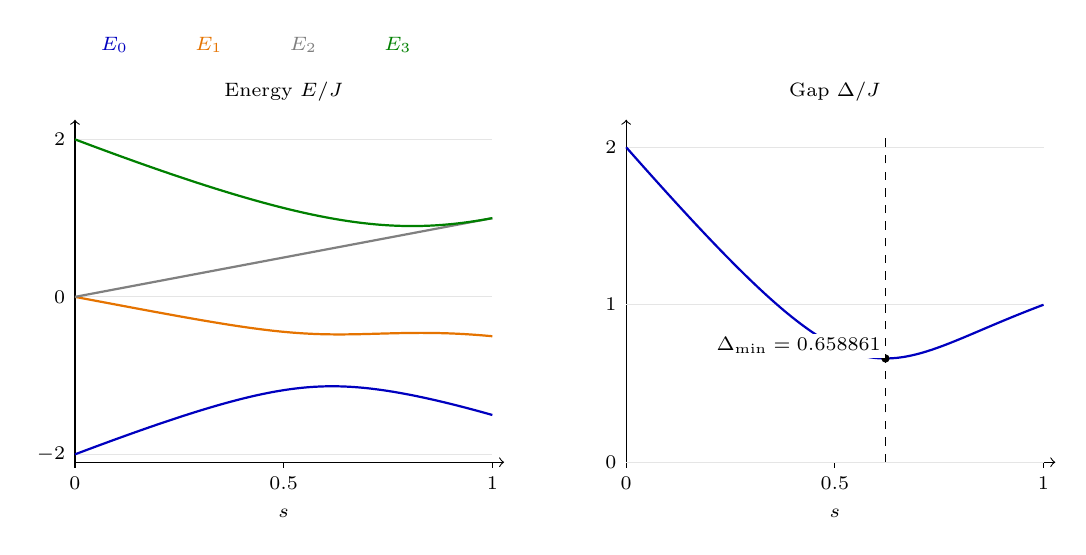
\begin{tikzpicture}[x=1cm,y=1cm,font=\scriptsize]
\draw[->] (0.0000,0.0000)--(5.4500,0.0000);
\draw[->] (0.0000,0.0000)--(0.0000,4.3500);
\draw (0.0000,0.0000)--+(0,-.07) node[below] {$0$};
\draw (2.6500,0.0000)--+(0,-.07) node[below] {$0.5$};
\draw (5.3000,0.0000)--+(0,-.07) node[below] {$1$};
\draw[gray!20] (0.0000,0.1000)--+(5.3000,0);
\node[left] at (0.0000,0.1000) {$-2$};
\draw[gray!20] (0.0000,2.1000)--+(5.3000,0);
\node[left] at (0.0000,2.1000) {$0$};
\draw[gray!20] (0.0000,4.1000)--+(5.3000,0);
\node[left] at (0.0000,4.1000) {$2$};
\node at (2.6500,-0.6500) {$s$};
\node at (2.6500,4.7000) {\lr{Energy} $E/J$};
\draw[blue!75!black,thick,] plot coordinates {(0.00000,0.10000) (0.02650,0.10999) (0.05300,0.11997) (0.07950,0.12993) (0.10600,0.13987) (0.13250,0.14980) (0.15900,0.15971) (0.18550,0.16960) (0.21200,0.17947) (0.23850,0.18933) (0.26500,0.19917) (0.29150,0.20899) (0.31800,0.21879) (0.34450,0.22857) (0.37100,0.23833) (0.39750,0.24807) (0.42400,0.25779) (0.45050,0.26749) (0.47700,0.27716) (0.50350,0.28682) (0.53000,0.29645) (0.55650,0.30606) (0.58300,0.31565) (0.60950,0.32521) (0.63600,0.33475) (0.66250,0.34426) (0.68900,0.35375) (0.71550,0.36321) (0.74200,0.37264) (0.76850,0.38205) (0.79500,0.39143) (0.82150,0.40078) (0.84800,0.41011) (0.87450,0.41940) (0.90100,0.42866) (0.92750,0.43790) (0.95400,0.44710) (0.98050,0.45627) (1.00700,0.46541) (1.03350,0.47451) (1.06000,0.48358) (1.08650,0.49261) (1.11300,0.50161) (1.13950,0.51057) (1.16600,0.51949) (1.19250,0.52837) (1.21900,0.53722) (1.24550,0.54602) (1.27200,0.55478) (1.29850,0.56350) (1.32500,0.57218) (1.35150,0.58081) (1.37800,0.58940) (1.40450,0.59793) (1.43100,0.60642) (1.45750,0.61487) (1.48400,0.62326) (1.51050,0.63160) (1.53700,0.63988) (1.56350,0.64811) (1.59000,0.65629) (1.61650,0.66441) (1.64300,0.67247) (1.66950,0.68046) (1.69600,0.68840) (1.72250,0.69628) (1.74900,0.70408) (1.77550,0.71182) (1.80200,0.71950) (1.82850,0.72710) (1.85500,0.73463) (1.88150,0.74208) (1.90800,0.74946) (1.93450,0.75676) (1.96100,0.76398) (1.98750,0.77112) (2.01400,0.77817) (2.04050,0.78514) (2.06700,0.79201) (2.09350,0.79879) (2.12000,0.80548) (2.14650,0.81208) (2.17300,0.81857) (2.19950,0.82496) (2.22600,0.83124) (2.25250,0.83742) (2.27900,0.84349) (2.30550,0.84944) (2.33200,0.85528) (2.35850,0.86100) (2.38500,0.86660) (2.41150,0.87207) (2.43800,0.87741) (2.46450,0.88263) (2.49100,0.88771) (2.51750,0.89265) (2.54400,0.89745) (2.57050,0.90211) (2.59700,0.90662) (2.62350,0.91098) (2.65000,0.91519) (2.67650,0.91925) (2.70300,0.92315) (2.72950,0.92688) (2.75600,0.93045) (2.78250,0.93386) (2.80900,0.93710) (2.83550,0.94016) (2.86200,0.94306) (2.88850,0.94577) (2.91500,0.94831) (2.94150,0.95067) (2.96800,0.95285) (2.99450,0.95485) (3.02100,0.95666) (3.04750,0.95829) (3.07400,0.95973) (3.10050,0.96098) (3.12700,0.96205) (3.15350,0.96293) (3.18000,0.96362) (3.20650,0.96413) (3.23300,0.96445) (3.25950,0.96459) (3.28600,0.96454) (3.31250,0.96430) (3.33900,0.96389) (3.36550,0.96329) (3.39200,0.96252) (3.41850,0.96156) (3.44500,0.96044) (3.47150,0.95914) (3.49800,0.95767) (3.52450,0.95603) (3.55100,0.95422) (3.57750,0.95226) (3.60400,0.95013) (3.63050,0.94785) (3.65700,0.94541) (3.68350,0.94282) (3.71000,0.94009) (3.73650,0.93721) (3.76300,0.93418) (3.78950,0.93102) (3.81600,0.92772) (3.84250,0.92429) (3.86900,0.92073) (3.89550,0.91705) (3.92200,0.91324) (3.94850,0.90930) (3.97500,0.90526) (4.00150,0.90109) (4.02800,0.89682) (4.05450,0.89243) (4.08100,0.88794) (4.10750,0.88334) (4.13400,0.87864) (4.16050,0.87385) (4.18700,0.86896) (4.21350,0.86397) (4.24000,0.85889) (4.26650,0.85372) (4.29300,0.84847) (4.31950,0.84313) (4.34600,0.83770) (4.37250,0.83220) (4.39900,0.82661) (4.42550,0.82095) (4.45200,0.81521) (4.47850,0.80940) (4.50500,0.80352) (4.53150,0.79757) (4.55800,0.79154) (4.58450,0.78545) (4.61100,0.77930) (4.63750,0.77308) (4.66400,0.76679) (4.69050,0.76045) (4.71700,0.75405) (4.74350,0.74758) (4.77000,0.74106) (4.79650,0.73448) (4.82300,0.72785) (4.84950,0.72116) (4.87600,0.71441) (4.90250,0.70762) (4.92900,0.70077) (4.95550,0.69388) (4.98200,0.68693) (5.00850,0.67994) (5.03500,0.67289) (5.06150,0.66580) (5.08800,0.65867) (5.11450,0.65148) (5.14100,0.64426) (5.16750,0.63699) (5.19400,0.62967) (5.22050,0.62232) (5.24700,0.61492) (5.27350,0.60748) (5.30000,0.60000)};
\node[text=blue!75!black] at (0.50,5.3) {$E_0$};
\draw[orange!90!black,thick,] plot coordinates {(0.00000,2.10000) (0.02650,2.09500) (0.05300,2.09000) (0.07950,2.08500) (0.10600,2.08000) (0.13250,2.07500) (0.15900,2.07000) (0.18550,2.06501) (0.21200,2.06001) (0.23850,2.05501) (0.26500,2.05002) (0.29150,2.04502) (0.31800,2.04003) (0.34450,2.03504) (0.37100,2.03005) (0.39750,2.02506) (0.42400,2.02008) (0.45050,2.01509) (0.47700,2.01011) (0.50350,2.00513) (0.53000,2.00015) (0.55650,1.99518) (0.58300,1.99021) (0.60950,1.98524) (0.63600,1.98028) (0.66250,1.97532) (0.68900,1.97036) (0.71550,1.96541) (0.74200,1.96046) (0.76850,1.95552) (0.79500,1.95058) (0.82150,1.94565) (0.84800,1.94072) (0.87450,1.93580) (0.90100,1.93089) (0.92750,1.92598) (0.95400,1.92108) (0.98050,1.91619) (1.00700,1.91130) (1.03350,1.90642) (1.06000,1.90156) (1.08650,1.89670) (1.11300,1.89185) (1.13950,1.88701) (1.16600,1.88218) (1.19250,1.87736) (1.21900,1.87255) (1.24550,1.86775) (1.27200,1.86297) (1.29850,1.85820) (1.32500,1.85345) (1.35150,1.84870) (1.37800,1.84398) (1.40450,1.83927) (1.43100,1.83457) (1.45750,1.82990) (1.48400,1.82524) (1.51050,1.82060) (1.53700,1.81598) (1.56350,1.81137) (1.59000,1.80680) (1.61650,1.80224) (1.64300,1.79771) (1.66950,1.79320) (1.69600,1.78871) (1.72250,1.78425) (1.74900,1.77982) (1.77550,1.77542) (1.80200,1.77105) (1.82850,1.76671) (1.85500,1.76240) (1.88150,1.75812) (1.90800,1.75388) (1.93450,1.74968) (1.96100,1.74551) (1.98750,1.74138) (2.01400,1.73729) (2.04050,1.73325) (2.06700,1.72925) (2.09350,1.72529) (2.12000,1.72138) (2.14650,1.71752) (2.17300,1.71371) (2.19950,1.70995) (2.22600,1.70625) (2.25250,1.70261) (2.27900,1.69902) (2.30550,1.69549) (2.33200,1.69203) (2.35850,1.68862) (2.38500,1.68529) (2.41150,1.68202) (2.43800,1.67883) (2.46450,1.67570) (2.49100,1.67265) (2.51750,1.66968) (2.54400,1.66678) (2.57050,1.66397) (2.59700,1.66124) (2.62350,1.65859) (2.65000,1.65603) (2.67650,1.65356) (2.70300,1.65118) (2.72950,1.64889) (2.75600,1.64669) (2.78250,1.64459) (2.80900,1.64259) (2.83550,1.64068) (2.86200,1.63887) (2.88850,1.63716) (2.91500,1.63555) (2.94150,1.63404) (2.96800,1.63263) (2.99450,1.63132) (3.02100,1.63011) (3.04750,1.62900) (3.07400,1.62800) (3.10050,1.62709) (3.12700,1.62628) (3.15350,1.62557) (3.18000,1.62495) (3.20650,1.62443) (3.23300,1.62400) (3.25950,1.62366) (3.28600,1.62341) (3.31250,1.62324) (3.33900,1.62315) (3.36550,1.62314) (3.39200,1.62321) (3.41850,1.62335) (3.44500,1.62356) (3.47150,1.62384) (3.49800,1.62418) (3.52450,1.62457) (3.55100,1.62502) (3.57750,1.62551) (3.60400,1.62606) (3.63050,1.62664) (3.65700,1.62726) (3.68350,1.62791) (3.71000,1.62859) (3.73650,1.62929) (3.76300,1.63001) (3.78950,1.63074) (3.81600,1.63148) (3.84250,1.63223) (3.86900,1.63298) (3.89550,1.63373) (3.92200,1.63447) (3.94850,1.63520) (3.97500,1.63592) (4.00150,1.63662) (4.02800,1.63729) (4.05450,1.63794) (4.08100,1.63855) (4.10750,1.63914) (4.13400,1.63969) (4.16050,1.64020) (4.18700,1.64066) (4.21350,1.64108) (4.24000,1.64145) (4.26650,1.64177) (4.29300,1.64204) (4.31950,1.64225) (4.34600,1.64241) (4.37250,1.64250) (4.39900,1.64253) (4.42550,1.64249) (4.45200,1.64239) (4.47850,1.64222) (4.50500,1.64199) (4.53150,1.64168) (4.55800,1.64130) (4.58450,1.64085) (4.61100,1.64032) (4.63750,1.63972) (4.66400,1.63905) (4.69050,1.63830) (4.71700,1.63747) (4.74350,1.63656) (4.77000,1.63558) (4.79650,1.63452) (4.82300,1.63338) (4.84950,1.63217) (4.87600,1.63088) (4.90250,1.62951) (4.92900,1.62806) (4.95550,1.62654) (4.98200,1.62494) (5.00850,1.62326) (5.03500,1.62151) (5.06150,1.61969) (5.08800,1.61779) (5.11450,1.61581) (5.14100,1.61377) (5.16750,1.61165) (5.19400,1.60946) (5.22050,1.60720) (5.24700,1.60487) (5.27350,1.60247) (5.30000,1.60000)};
\node[text=orange!90!black] at (1.70,5.3) {$E_1$};
\draw[gray,thick,] plot coordinates {(0.00000,2.10000) (0.02650,2.10500) (0.05300,2.11000) (0.07950,2.11500) (0.10600,2.12000) (0.13250,2.12500) (0.15900,2.13000) (0.18550,2.13500) (0.21200,2.14000) (0.23850,2.14500) (0.26500,2.15000) (0.29150,2.15500) (0.31800,2.16000) (0.34450,2.16500) (0.37100,2.17000) (0.39750,2.17500) (0.42400,2.18000) (0.45050,2.18500) (0.47700,2.19000) (0.50350,2.19500) (0.53000,2.20000) (0.55650,2.20500) (0.58300,2.21000) (0.60950,2.21500) (0.63600,2.22000) (0.66250,2.22500) (0.68900,2.23000) (0.71550,2.23500) (0.74200,2.24000) (0.76850,2.24500) (0.79500,2.25000) (0.82150,2.25500) (0.84800,2.26000) (0.87450,2.26500) (0.90100,2.27000) (0.92750,2.27500) (0.95400,2.28000) (0.98050,2.28500) (1.00700,2.29000) (1.03350,2.29500) (1.06000,2.30000) (1.08650,2.30500) (1.11300,2.31000) (1.13950,2.31500) (1.16600,2.32000) (1.19250,2.32500) (1.21900,2.33000) (1.24550,2.33500) (1.27200,2.34000) (1.29850,2.34500) (1.32500,2.35000) (1.35150,2.35500) (1.37800,2.36000) (1.40450,2.36500) (1.43100,2.37000) (1.45750,2.37500) (1.48400,2.38000) (1.51050,2.38500) (1.53700,2.39000) (1.56350,2.39500) (1.59000,2.40000) (1.61650,2.40500) (1.64300,2.41000) (1.66950,2.41500) (1.69600,2.42000) (1.72250,2.42500) (1.74900,2.43000) (1.77550,2.43500) (1.80200,2.44000) (1.82850,2.44500) (1.85500,2.45000) (1.88150,2.45500) (1.90800,2.46000) (1.93450,2.46500) (1.96100,2.47000) (1.98750,2.47500) (2.01400,2.48000) (2.04050,2.48500) (2.06700,2.49000) (2.09350,2.49500) (2.12000,2.50000) (2.14650,2.50500) (2.17300,2.51000) (2.19950,2.51500) (2.22600,2.52000) (2.25250,2.52500) (2.27900,2.53000) (2.30550,2.53500) (2.33200,2.54000) (2.35850,2.54500) (2.38500,2.55000) (2.41150,2.55500) (2.43800,2.56000) (2.46450,2.56500) (2.49100,2.57000) (2.51750,2.57500) (2.54400,2.58000) (2.57050,2.58500) (2.59700,2.59000) (2.62350,2.59500) (2.65000,2.60000) (2.67650,2.60500) (2.70300,2.61000) (2.72950,2.61500) (2.75600,2.62000) (2.78250,2.62500) (2.80900,2.63000) (2.83550,2.63500) (2.86200,2.64000) (2.88850,2.64500) (2.91500,2.65000) (2.94150,2.65500) (2.96800,2.66000) (2.99450,2.66500) (3.02100,2.67000) (3.04750,2.67500) (3.07400,2.68000) (3.10050,2.68500) (3.12700,2.69000) (3.15350,2.69500) (3.18000,2.70000) (3.20650,2.70500) (3.23300,2.71000) (3.25950,2.71500) (3.28600,2.72000) (3.31250,2.72500) (3.33900,2.73000) (3.36550,2.73500) (3.39200,2.74000) (3.41850,2.74500) (3.44500,2.75000) (3.47150,2.75500) (3.49800,2.76000) (3.52450,2.76500) (3.55100,2.77000) (3.57750,2.77500) (3.60400,2.78000) (3.63050,2.78500) (3.65700,2.79000) (3.68350,2.79500) (3.71000,2.80000) (3.73650,2.80500) (3.76300,2.81000) (3.78950,2.81500) (3.81600,2.82000) (3.84250,2.82500) (3.86900,2.83000) (3.89550,2.83500) (3.92200,2.84000) (3.94850,2.84500) (3.97500,2.85000) (4.00150,2.85500) (4.02800,2.86000) (4.05450,2.86500) (4.08100,2.87000) (4.10750,2.87500) (4.13400,2.88000) (4.16050,2.88500) (4.18700,2.89000) (4.21350,2.89500) (4.24000,2.90000) (4.26650,2.90500) (4.29300,2.91000) (4.31950,2.91500) (4.34600,2.92000) (4.37250,2.92500) (4.39900,2.93000) (4.42550,2.93500) (4.45200,2.94000) (4.47850,2.94500) (4.50500,2.95000) (4.53150,2.95500) (4.55800,2.96000) (4.58450,2.96500) (4.61100,2.97000) (4.63750,2.97500) (4.66400,2.98000) (4.69050,2.98500) (4.71700,2.99000) (4.74350,2.99500) (4.77000,3.00000) (4.79650,3.00500) (4.82300,3.01000) (4.84950,3.01500) (4.87600,3.02000) (4.90250,3.02500) (4.92900,3.03000) (4.95550,3.03500) (4.98200,3.04000) (5.00850,3.04500) (5.03500,3.05000) (5.06150,3.05500) (5.08800,3.06000) (5.11450,3.06500) (5.14100,3.07000) (5.16750,3.07500) (5.19400,3.08000) (5.22050,3.08500) (5.24700,3.09000) (5.27350,3.09500) (5.30000,3.10000)};
\node[text=gray] at (2.90,5.3) {$E_2$};
\draw[green!50!black,thick,] plot coordinates {(0.00000,4.10000) (0.02650,4.09001) (0.05300,4.08003) (0.07950,4.07007) (0.10600,4.06013) (0.13250,4.05020) (0.15900,4.04029) (0.18550,4.03039) (0.21200,4.02052) (0.23850,4.01066) (0.26500,4.00081) (0.29150,3.99099) (0.31800,3.98118) (0.34450,3.97139) (0.37100,3.96162) (0.39750,3.95187) (0.42400,3.94214) (0.45050,3.93242) (0.47700,3.92273) (0.50350,3.91305) (0.53000,3.90340) (0.55650,3.89376) (0.58300,3.88415) (0.60950,3.87455) (0.63600,3.86498) (0.66250,3.85542) (0.68900,3.84589) (0.71550,3.83638) (0.74200,3.82689) (0.76850,3.81743) (0.79500,3.80799) (0.82150,3.79857) (0.84800,3.78917) (0.87450,3.77980) (0.90100,3.77045) (0.92750,3.76112) (0.95400,3.75182) (0.98050,3.74254) (1.00700,3.73329) (1.03350,3.72407) (1.06000,3.71487) (1.08650,3.70569) (1.11300,3.69655) (1.13950,3.68743) (1.16600,3.67833) (1.19250,3.66927) (1.21900,3.66023) (1.24550,3.65122) (1.27200,3.64225) (1.29850,3.63330) (1.32500,3.62438) (1.35150,3.61549) (1.37800,3.60663) (1.40450,3.59780) (1.43100,3.58900) (1.45750,3.58024) (1.48400,3.57151) (1.51050,3.56281) (1.53700,3.55414) (1.56350,3.54551) (1.59000,3.53692) (1.61650,3.52835) (1.64300,3.51983) (1.66950,3.51134) (1.69600,3.50289) (1.72250,3.49447) (1.74900,3.48609) (1.77550,3.47775) (1.80200,3.46945) (1.82850,3.46119) (1.85500,3.45297) (1.88150,3.44479) (1.90800,3.43666) (1.93450,3.42856) (1.96100,3.42051) (1.98750,3.41250) (2.01400,3.40454) (2.04050,3.39662) (2.06700,3.38874) (2.09350,3.38092) (2.12000,3.37314) (2.14650,3.36540) (2.17300,3.35772) (2.19950,3.35009) (2.22600,3.34250) (2.25250,3.33497) (2.27900,3.32749) (2.30550,3.32007) (2.33200,3.31269) (2.35850,3.30538) (2.38500,3.29812) (2.41150,3.29091) (2.43800,3.28376) (2.46450,3.27667) (2.49100,3.26964) (2.51750,3.26267) (2.54400,3.25577) (2.57050,3.24892) (2.59700,3.24214) (2.62350,3.23542) (2.65000,3.22877) (2.67650,3.22219) (2.70300,3.21567) (2.72950,3.20923) (2.75600,3.20285) (2.78250,3.19655) (2.80900,3.19031) (2.83550,3.18416) (2.86200,3.17807) (2.88850,3.17207) (2.91500,3.16614) (2.94150,3.16029) (2.96800,3.15452) (2.99450,3.14883) (3.02100,3.14323) (3.04750,3.13771) (3.07400,3.13228) (3.10050,3.12693) (3.12700,3.12167) (3.15350,3.11650) (3.18000,3.11142) (3.20650,3.10644) (3.23300,3.10155) (3.25950,3.09676) (3.28600,3.09206) (3.31250,3.08746) (3.33900,3.08296) (3.36550,3.07856) (3.39200,3.07427) (3.41850,3.07008) (3.44500,3.06600) (3.47150,3.06202) (3.49800,3.05816) (3.52450,3.05440) (3.55100,3.05076) (3.57750,3.04723) (3.60400,3.04381) (3.63050,3.04051) (3.65700,3.03733) (3.68350,3.03427) (3.71000,3.03133) (3.73650,3.02851) (3.76300,3.02581) (3.78950,3.02324) (3.81600,3.02079) (3.84250,3.01847) (3.86900,3.01628) (3.89550,3.01422) (3.92200,3.01229) (3.94850,3.01049) (3.97500,3.00883) (4.00150,3.00729) (4.02800,3.00590) (4.05450,3.00463) (4.08100,3.00351) (4.10750,3.00252) (4.13400,3.00167) (4.16050,3.00096) (4.18700,3.00038) (4.21350,2.99995) (4.24000,2.99966) (4.26650,2.99950) (4.29300,2.99949) (4.31950,2.99962) (4.34600,2.99989) (4.37250,3.00031) (4.39900,3.00086) (4.42550,3.00156) (4.45200,3.00240) (4.47850,3.00337) (4.50500,3.00449) (4.53150,3.00576) (4.55800,3.00716) (4.58450,3.00870) (4.61100,3.01038) (4.63750,3.01220) (4.66400,3.01416) (4.69050,3.01625) (4.71700,3.01849) (4.74350,3.02086) (4.77000,3.02336) (4.79650,3.02600) (4.82300,3.02877) (4.84950,3.03167) (4.87600,3.03471) (4.90250,3.03787) (4.92900,3.04116) (4.95550,3.04458) (4.98200,3.04813) (5.00850,3.05180) (5.03500,3.05560) (5.06150,3.05951) (5.08800,3.06355) (5.11450,3.06770) (5.14100,3.07198) (5.16750,3.07637) (5.19400,3.08087) (5.22050,3.08549) (5.24700,3.09022) (5.27350,3.09505) (5.30000,3.10000)};
\node[text=green!50!black] at (4.10,5.3) {$E_3$};
\draw[->] (7.0000,0.0000)--(12.4500,0.0000);
\draw[->] (7.0000,0.0000)--(7.0000,4.3500);
\draw (7.0000,0.0000)--+(0,-.07) node[below] {$0$};
\draw (9.6500,0.0000)--+(0,-.07) node[below] {$0.5$};
\draw (12.3000,0.0000)--+(0,-.07) node[below] {$1$};
\draw[gray!20] (7.0000,0.0000)--+(5.3000,0);
\node[left] at (7.0000,0.0000) {$0$};
\draw[gray!20] (7.0000,2.0000)--+(5.3000,0);
\node[left] at (7.0000,2.0000) {$1$};
\draw[gray!20] (7.0000,4.0000)--+(5.3000,0);
\node[left] at (7.0000,4.0000) {$2$};
\node at (9.6500,-0.6500) {$s$};
\node at (9.6500,4.7000) {\lr{Gap} $\Delta/J$};
\draw[blue!75!black,thick,] plot coordinates {(7.00000,4.00000) (7.02650,3.97002) (7.05300,3.94006) (7.07950,3.91014) (7.10600,3.88026) (7.13250,3.85041) (7.15900,3.82059) (7.18550,3.79081) (7.21200,3.76107) (7.23850,3.73136) (7.26500,3.70170) (7.29150,3.67207) (7.31800,3.64249) (7.34450,3.61294) (7.37100,3.58344) (7.39750,3.55399) (7.42400,3.52458) (7.45050,3.49521) (7.47700,3.46589) (7.50350,3.43663) (7.53000,3.40741) (7.55650,3.37824) (7.58300,3.34913) (7.60950,3.32007) (7.63600,3.29107) (7.66250,3.26212) (7.68900,3.23323) (7.71550,3.20441) (7.74200,3.17564) (7.76850,3.14694) (7.79500,3.11830) (7.82150,3.08973) (7.84800,3.06123) (7.87450,3.03280) (7.90100,3.00445) (7.92750,2.97617) (7.95400,2.94796) (7.98050,2.91984) (8.00700,2.89179) (8.03350,2.86383) (8.06000,2.83596) (8.08650,2.80817) (8.11300,2.78048) (8.13950,2.75288) (8.16600,2.72537) (8.19250,2.69797) (8.21900,2.67066) (8.24550,2.64347) (8.27200,2.61638) (8.29850,2.58940) (8.32500,2.56253) (8.35150,2.53579) (8.37800,2.50916) (8.40450,2.48267) (8.43100,2.45630) (8.45750,2.43006) (8.48400,2.40396) (8.51050,2.37800) (8.53700,2.35219) (8.56350,2.32652) (8.59000,2.30102) (8.61650,2.27567) (8.64300,2.25048) (8.66950,2.22546) (8.69600,2.20062) (8.72250,2.17596) (8.74900,2.15148) (8.77550,2.12719) (8.80200,2.10310) (8.82850,2.07922) (8.85500,2.05554) (8.88150,2.03208) (8.90800,2.00884) (8.93450,1.98583) (8.96100,1.96305) (8.98750,1.94052) (9.01400,1.91824) (9.04050,1.89622) (9.06700,1.87447) (9.09350,1.85299) (9.12000,1.83180) (9.14650,1.81089) (9.17300,1.79029) (9.19950,1.77000) (9.22600,1.75002) (9.25250,1.73037) (9.27900,1.71106) (9.30550,1.69210) (9.33200,1.67349) (9.35850,1.65525) (9.38500,1.63738) (9.41150,1.61991) (9.43800,1.60283) (9.46450,1.58615) (9.49100,1.56989) (9.51750,1.55406) (9.54400,1.53867) (9.57050,1.52373) (9.59700,1.50924) (9.62350,1.49522) (9.65000,1.48168) (9.67650,1.46863) (9.70300,1.45607) (9.72950,1.44402) (9.75600,1.43248) (9.78250,1.42146) (9.80900,1.41098) (9.83550,1.40103) (9.86200,1.39162) (9.88850,1.38277) (9.91500,1.37447) (9.94150,1.36673) (9.96800,1.35955) (9.99450,1.35294) (10.02100,1.34691) (10.04750,1.34144) (10.07400,1.33654) (10.10050,1.33222) (10.12700,1.32846) (10.15350,1.32528) (10.18000,1.32266) (10.20650,1.32060) (10.23300,1.31910) (10.25950,1.31815) (10.28600,1.31774) (10.31250,1.31787) (10.33900,1.31853) (10.36550,1.31971) (10.39200,1.32139) (10.41850,1.32358) (10.44500,1.32625) (10.47150,1.32941) (10.49800,1.33302) (10.52450,1.33708) (10.55100,1.34159) (10.57750,1.34651) (10.60400,1.35185) (10.63050,1.35758) (10.65700,1.36369) (10.68350,1.37017) (10.71000,1.37700) (10.73650,1.38416) (10.76300,1.39165) (10.78950,1.39944) (10.81600,1.40752) (10.84250,1.41588) (10.86900,1.42450) (10.89550,1.43337) (10.92200,1.44248) (10.94850,1.45180) (10.97500,1.46133) (11.00150,1.47105) (11.02800,1.48095) (11.05450,1.49101) (11.08100,1.50123) (11.10750,1.51159) (11.13400,1.52208) (11.16050,1.53269) (11.18700,1.54341) (11.21350,1.55423) (11.24000,1.56513) (11.26650,1.57611) (11.29300,1.58715) (11.31950,1.59825) (11.34600,1.60941) (11.37250,1.62060) (11.39900,1.63183) (11.42550,1.64309) (11.45200,1.65436) (11.47850,1.66564) (11.50500,1.67694) (11.53150,1.68823) (11.55800,1.69951) (11.58450,1.71079) (11.61100,1.72205) (11.63750,1.73329) (11.66400,1.74450) (11.69050,1.75569) (11.71700,1.76684) (11.74350,1.77796) (11.77000,1.78904) (11.79650,1.80008) (11.82300,1.81108) (11.84950,1.82203) (11.87600,1.83293) (11.90250,1.84378) (11.92900,1.85458) (11.95550,1.86532) (11.98200,1.87602) (12.00850,1.88666) (12.03500,1.89724) (12.06150,1.90777) (12.08800,1.91824) (12.11450,1.92866) (12.14100,1.93902) (12.16750,1.94932) (12.19400,1.95957) (12.22050,1.96976) (12.24700,1.97989) (12.27350,1.98997) (12.30000,2.00000)};
\draw[dashed] (10.2928,0)--(10.2928,4.2); \fill (10.2928,1.3177) circle (1.5pt);
\node[above left,fill=white,inner sep=1.5pt] at (10.2928,1.3177) {$\Delta_{\min}=0.658861$};
\end{tikzpicture}
	\caption{طیف و گاف محاسبه‌شده دو اسپین برای $h_z=1/4$؛ خط عمودی محل کمینه است. این شکل طرحواره نیست.}
	\label{fig:gap-computed-spectrum}
\end{figure}

\subsection{کمینه‌سازی روی مسیر و خطای شبکه}
تمام بازه و دو انتها را بررسی و اطراف همه کمینه‌های محتمل شبکه را ریز کنید.
کمینه شبکه کران بالای کمینه پیوسته است و ممکن است گلوگاهی باریک را از دست بدهد.
اگر $\|H'(s)\|\leq L_H$، نامساوی ویل می‌دهد:
\begin{equation}
	|\Delta(s)-\Delta(s')|\leq2L_H|s-s'|.
\end{equation}
برای شبکه شامل دو انتها با بیشینه فاصله $h$:
\begin{equation}
	\max(0,\Delta_{\mathrm{grid}}-L_Hh)\leq\Delta_{\min}\leq\Delta_{\mathrm{grid}}.
	\label{eq:gap-grid-bound}
\end{equation}
با خطای حداکثر $\epsilon_g$ در هر گاف نمونه، از کران پایین $\epsilon_g$ کم و به بالا اضافه می‌شود.
برای کمینه هموار داخلی، هلمان--فاینمن می‌دهد:
\begin{equation}
	\Delta'(s)=\langle1|H'|1\rangle-\langle0|H'|0\rangle.
\end{equation}
ریشه مشتق فقط نامزد کمینه است؛ نقاط مرزی هم باید مقایسه شوند. در تبهگنی، بخش‌های تقارنی را جدا دنبال کنید.

\subsection{آزمون مستقیم زمان‌بندی}
شرودینگر را برای چند $T$ حل می‌کنیم. انتشار هر ریزگام با نماییِ هامیلتونیِ نقطه میانی انجام و با نصف‌کردن گام، همگرایی بررسی می‌شود. قطعات پائولی در این محاسبه تروتر نشده‌اند.
\begin{equation}
	P_{\mathrm{succ}}(T)=|\langle00|\Psi(T)\rangle|^2.
\end{equation}
شکل~\ref{fig:gap-schedule-test} جاروب خطی و زمان‌بندی مبتنی بر
$\max\{K,0.05\max K\}$ را در زمان کل برابر مقایسه می‌کند.
زمان‌بندی محلی در هر $T$ الزاماً بهتر نیست؛ تداخل گذارها می‌تواند موفقیت را نوسانی کند.
عدد مرتبه‌ای $T\sim500$ در مثال قبلی، کمترین زمان موفقیت نیست.
\begin{figure}[htbp]
	\centering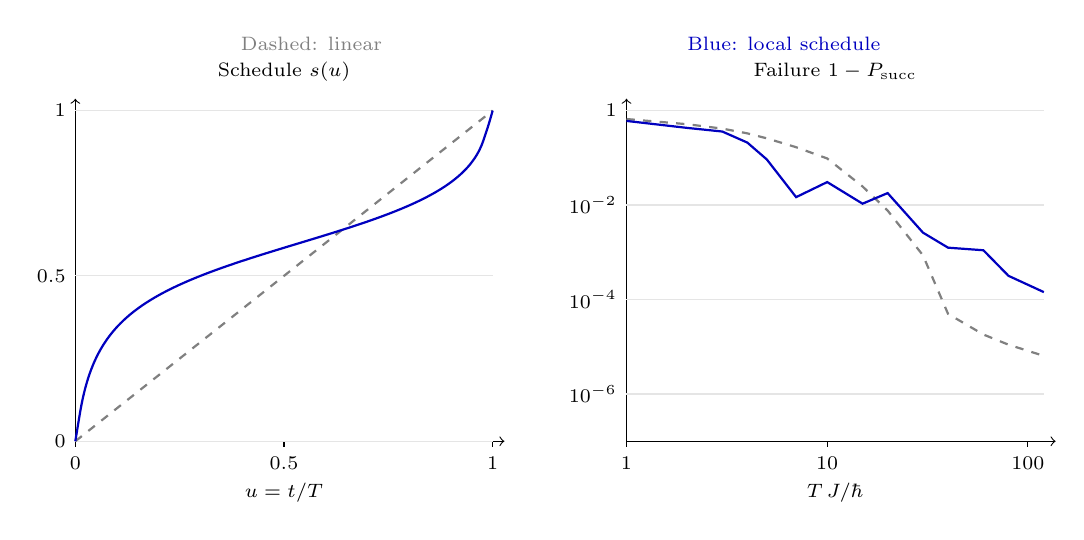
\begin{tikzpicture}[x=1cm,y=1cm,font=\scriptsize]
\draw[->] (0.0000,0.0000)--(5.4500,0.0000);
\draw[->] (0.0000,0.0000)--(0.0000,4.3500);
\draw (0.0000,0.0000)--+(0,-.07) node[below] {$0$};
\draw (2.6500,0.0000)--+(0,-.07) node[below] {$0.5$};
\draw (5.3000,0.0000)--+(0,-.07) node[below] {$1$};
\draw[gray!20] (0.0000,0.0000)--+(5.3000,0);
\node[left] at (0.0000,0.0000) {$0$};
\draw[gray!20] (0.0000,2.1000)--+(5.3000,0);
\node[left] at (0.0000,2.1000) {$0.5$};
\draw[gray!20] (0.0000,4.2000)--+(5.3000,0);
\node[left] at (0.0000,4.2000) {$1$};
\node at (2.6500,-0.6500) {$u=t/T$};
\node at (2.6500,4.7000) {\lr{Schedule} $s(u)$};
\draw[gray,thick,dashed] plot coordinates {(0.00000,0.00000) (5.30000,4.20000)};
\draw[blue!75!black,thick,] plot coordinates {(0.00000,0.00000) (0.00346,0.02100) (0.00692,0.04200) (0.01038,0.06300) (0.01384,0.08400) (0.01730,0.10500) (0.02076,0.12600) (0.02422,0.14700) (0.02768,0.16800) (0.03114,0.18900) (0.03460,0.21000) (0.03806,0.23100) (0.04152,0.25200) (0.04498,0.27300) (0.04844,0.29400) (0.05190,0.31500) (0.05536,0.33600) (0.05886,0.35700) (0.06245,0.37800) (0.06615,0.39900) (0.06996,0.42000) (0.07389,0.44100) (0.07793,0.46200) (0.08209,0.48300) (0.08637,0.50400) (0.09078,0.52500) (0.09533,0.54600) (0.10001,0.56700) (0.10484,0.58800) (0.10982,0.60900) (0.11495,0.63000) (0.12024,0.65100) (0.12570,0.67200) (0.13132,0.69300) (0.13713,0.71400) (0.14312,0.73500) (0.14930,0.75600) (0.15568,0.77700) (0.16226,0.79800) (0.16906,0.81900) (0.17608,0.84000) (0.18333,0.86100) (0.19082,0.88200) (0.19855,0.90300) (0.20655,0.92400) (0.21481,0.94500) (0.22334,0.96600) (0.23217,0.98700) (0.24129,1.00800) (0.25072,1.02900) (0.26048,1.05000) (0.27057,1.07100) (0.28101,1.09200) (0.29181,1.11300) (0.30299,1.13400) (0.31455,1.15500) (0.32653,1.17600) (0.33892,1.19700) (0.35175,1.21800) (0.36503,1.23900) (0.37879,1.26000) (0.39304,1.28100) (0.40779,1.30200) (0.42308,1.32300) (0.43891,1.34400) (0.45532,1.36500) (0.47232,1.38600) (0.48993,1.40700) (0.50817,1.42800) (0.52708,1.44900) (0.54668,1.47000) (0.56699,1.49100) (0.58803,1.51200) (0.60983,1.53300) (0.63243,1.55400) (0.65584,1.57500) (0.68010,1.59600) (0.70523,1.61700) (0.73127,1.63800) (0.75824,1.65900) (0.78617,1.68000) (0.81510,1.70100) (0.84504,1.72200) (0.87604,1.74300) (0.90811,1.76400) (0.94130,1.78500) (0.97563,1.80600) (1.01112,1.82700) (1.04780,1.84800) (1.08570,1.86900) (1.12484,1.89000) (1.16524,1.91100) (1.20693,1.93200) (1.24992,1.95300) (1.29422,1.97400) (1.33986,1.99500) (1.38683,2.01600) (1.43515,2.03700) (1.48481,2.05800) (1.53582,2.07900) (1.58817,2.10000) (1.64183,2.12100) (1.69681,2.14200) (1.75307,2.16300) (1.81059,2.18400) (1.86934,2.20500) (1.92927,2.22600) (1.99034,2.24700) (2.05249,2.26800) (2.11568,2.28900) (2.17983,2.31000) (2.24488,2.33100) (2.31075,2.35200) (2.37736,2.37300) (2.44462,2.39400) (2.51245,2.41500) (2.58076,2.43600) (2.64944,2.45700) (2.71839,2.47800) (2.78751,2.49900) (2.85671,2.52000) (2.92587,2.54100) (2.99488,2.56200) (3.06366,2.58300) (3.13208,2.60400) (3.20006,2.62500) (3.26749,2.64600) (3.33429,2.66700) (3.40035,2.68800) (3.46559,2.70900) (3.52994,2.73000) (3.59331,2.75100) (3.65564,2.77200) (3.71686,2.79300) (3.77690,2.81400) (3.83572,2.83500) (3.89328,2.85600) (3.94951,2.87700) (4.00441,2.89800) (4.05792,2.91900) (4.11003,2.94000) (4.16072,2.96100) (4.20998,2.98200) (4.25780,3.00300) (4.30416,3.02400) (4.34908,3.04500) (4.39256,3.06600) (4.43459,3.08700) (4.47521,3.10800) (4.51441,3.12900) (4.55222,3.15000) (4.58865,3.17100) (4.62373,3.19200) (4.65747,3.21300) (4.68991,3.23400) (4.72106,3.25500) (4.75096,3.27600) (4.77964,3.29700) (4.80712,3.31800) (4.83343,3.33900) (4.85860,3.36000) (4.88266,3.38100) (4.90564,3.40200) (4.92758,3.42300) (4.94850,3.44400) (4.96843,3.46500) (4.98740,3.48600) (5.00544,3.50700) (5.02258,3.52800) (5.03885,3.54900) (5.05428,3.57000) (5.06889,3.59100) (5.08271,3.61200) (5.09576,3.63300) (5.10808,3.65400) (5.11969,3.67500) (5.13061,3.69600) (5.14086,3.71700) (5.15047,3.73800) (5.15946,3.75900) (5.16786,3.78000) (5.17568,3.80100) (5.18307,3.82200) (5.19036,3.84300) (5.19755,3.86400) (5.20464,3.88500) (5.21165,3.90600) (5.21856,3.92700) (5.22537,3.94800) (5.23210,3.96900) (5.23873,3.99000) (5.24527,4.01100) (5.25172,4.03200) (5.25808,4.05300) (5.26434,4.07400) (5.27052,4.09500) (5.27661,4.11600) (5.28261,4.13700) (5.28852,4.15800) (5.29434,4.17900) (5.30000,4.20000)};
\draw[->] (7.0000,0.0000)--(12.4500,0.0000);
\draw[->] (7.0000,0.0000)--(7.0000,4.3500);
\draw (7.0000,0.0000)--+(0,-.07) node[below] {$1$};
\draw (9.5491,0.0000)--+(0,-.07) node[below] {$10$};
\draw (12.0982,0.0000)--+(0,-.07) node[below] {$100$};
\draw[gray!20] (7.0000,0.6000)--+(5.3000,0);
\node[left] at (7.0000,0.6000) {$10^{-6}$};
\draw[gray!20] (7.0000,1.8000)--+(5.3000,0);
\node[left] at (7.0000,1.8000) {$10^{-4}$};
\draw[gray!20] (7.0000,3.0000)--+(5.3000,0);
\node[left] at (7.0000,3.0000) {$10^{-2}$};
\draw[gray!20] (7.0000,4.2000)--+(5.3000,0);
\node[left] at (7.0000,4.2000) {$1$};
\node at (9.6500,-0.6500) {$T\,J/\hbar$};
\node at (9.6500,4.7000) {\lr{Failure} $1-P_{\mathrm{succ}}$};
\draw[gray,thick,dashed] plot coordinates {(7.00000,4.09221) (7.76735,4.02687) (8.21622,3.97075) (8.53470,3.91043) (8.78173,3.84693) (9.15422,3.73444) (9.54908,3.59128) (9.99795,3.23601) (10.31643,2.92987) (10.76530,2.36095) (11.08378,1.61751) (11.53265,1.35560) (11.85113,1.22652) (12.30000,1.08434)};
\draw[blue!75!black,thick,] plot coordinates {(7.00000,4.06821) (7.76735,3.97998) (8.21622,3.93364) (8.53470,3.79306) (8.78173,3.57925) (9.15422,3.10026) (9.54908,3.29167) (9.99795,3.01712) (10.31643,3.15171) (10.76530,2.64937) (11.08378,2.45851) (11.53265,2.42579) (11.85113,2.10113) (12.30000,1.89413)};
\node[text=gray] at (3,5.05) {\lr{Dashed: linear}};
\node[text=blue!75!black] at (9,5.05) {\lr{Blue: local schedule}};
\end{tikzpicture}
	\caption{چپ: $s$ بر حسب زمان نرمال‌شده. راست: احتمال شکستِ دو زمان‌بندی در زمان کل برابر. مدل بسته و بی‌نویز است.}
	\label{fig:gap-schedule-test}
\end{figure}

\subsection{گاف صفر، ولی گذار ممنوع}
برای $h_z=0$ تقارن $\Pi=X_1X_2$ برقرار است و $|++\rangle$ در بخش زوج قرار دارد.
با $a=1-s,b=s$، انرژی‌ها
$\{-\sqrt{b^2+4a^2},-b,b,\sqrt{b^2+4a^2}\}$ هستند.
گاف کل $\sqrt{b^2+4a^2}-b$ در انتها صفر، اما گاف بخش زوج
$2\sqrt{b^2+4a^2}$ مثبت است.
هدف زوج $(|00\rangle+|11\rangle)/\sqrt2$ است، نه حالت یکتای $|00\rangle$.
اگر هدف مشخصاً $|00\rangle$ باشد باید تقارن شکسته شود؛ مسئله و گاف مرتبط تغییر می‌کند.

\section{روش‌های محاسبه گاف: انتخاب بر اساس ساختار}
\label{sec:gap-methods}
\subsection{قطری‌سازی، لانچوس و شبکه تانسوری}
برای $n$ کیوبیت، $D=2^n$ است. ماتریس متراکم حافظه $O(D^2)$ و قطری‌سازی کامل زمان نوعی $O(D^3)$ می‌خواهد.
برای $H=\sum_{\ell=1}^m c_\ell P_\ell$، ضرب $Hv$ را می‌توان بدون ساخت ماتریس با هزینه نوعی $O(mD)$ انجام داد.
در لانچوس، زیرفضای
\begin{equation}
	{\cal K}_k(H,v)=\mathrm{span}\{v,Hv,\ldots,H^{k-1}v\}
\end{equation}
از یک بردار شروع ساخته می‌شود. بازگشت
$Hv_j=\beta_jv_{j-1}+\alpha_jv_j+\beta_{j+1}v_{j+1}$
ماتریس سه‌قطری ایجاد می‌کند؛ کوچک‌ترین مقادیر ریتز تقریب ترازهای پایین‌اند.
چند بردار شروع، بازمتعامدسازی و محاسبه چند تراز کمک می‌کند یک تراز نزدیک یا بخش تقارنی جا نیفتد.
همگرایی به جدایی طیفی و هم‌پوشانی شروع وابسته است؛ تنکی، مشکل نماییِ بردار $D$بعدی را حذف نمی‌کند.

برای زوج تقریبی $(\widetilde E,v)$ با $\|v\|=1$:
\begin{equation}
	r=Hv-\widetilde Ev,\qquad
	\min_j|\widetilde E-E_j|\leq\|r\|.
\end{equation}
باقیمانده کوچک نزدیکی به یک ویژه‌مقدار را نشان می‌دهد، نه شناسایی قطعی $E_0$ یا $E_1$.
برای گاف گواهی‌شده، ترتیب ترازها یا کران‌های مستقل نیز لازم است.

در زنجیره‌های کم‌درهم‌تنیده، \lr{DMRG/MPS} مرجع کلاسیک مناسبی است: پایه و حالت برانگیخته در بخش تقارنی مشخص به‌صورت وردشی محاسبه می‌شوند.
همگرایی نسبت به بُعد پیوند $\chi$، طول زنجیره، تعداد جاروب و واریانس انرژی را بررسی کنید.
نزدیک بحرانی‌شدن یا برای درهم‌تنیدگی زیاد، $\chi$ لازم افزایش می‌یابد~\cite{GapSchollwock2011}.
مونت‌کارلو کوانتومی در مدل‌های بدون مشکل علامت نیز می‌تواند از افت همبستگی زمان موهومی گاف استخراج کند؛ بازسازی طیف از داده نویزی محدودیت دارد.

\subsection{گاف از همبستگی: کدام تراز دیده می‌شود؟}
همبستگی متصل زمان موهومی در پایه واقعی، برای $O$ هرمیتی:
\begin{equation}
	C_O(\tau)=\sum_{m>0}|\langle m|O|0\rangle|^2e^{-\Delta_{m0}\tau/\hbar}.
\end{equation}
در زمان بلند، شیب $-\hbar\,d\log C_O/d\tau$ به کمترین گاف دارای وزن غیرصفر میل می‌کند.
در زمان حقیقی همین فرکانس‌ها نوسانی‌اند. انتخاب $O$ مشخص می‌کند کدام بخش تقارنی دیده شود؛ نبود قله دلیل نبود تراز نیست.
در دمای غیرصفر، گذار از حالت‌های گرمایی نیز وارد می‌شود.

\subsection{\lr{QPE}، \lr{VQD} و قطری‌سازی زیرفضای کوانتومی}
در \lr{QPE} با $U=\exp[-i(H-E_{\mathrm{ref}})\tau/\hbar]$، بازه انرژی و زمان پایه باید رفع ابهام فاز را ممکن کنند.
برای دو تخمین با خطای مطلق $\epsilon_E$:
\begin{equation}
	|\widetilde\Delta-\Delta|\leq2\epsilon_E.
\end{equation}
دقت نسبی $r_\Delta$ نیازمند $\epsilon_E\lesssim r_\Delta\Delta/2$ است.
زمان همدوس نوعی نسخه استاندارد $O(\hbar/\epsilon_E)$ است؛ هزینه ساخت تحول و آماده‌سازی دو حالت با هم‌پوشانی کافی نیز اضافه می‌شود.
اگر هم‌پوشانی با تراز اول ناچیز باشد، تکرار QPE آن را به‌سادگی پیدا نمی‌کند.

\lr{VQE} معمولی فقط یک انرژی پایین را هدف می‌گیرد. در \lr{VQD}، هزینه
\begin{equation}
	{\cal L}_k(\theta)=\langle H\rangle_\theta+
	\sum_{j<k}\mu_j|\langle\psi_j|\psi(\theta)\rangle|^2
\end{equation}
حالت‌های پایین‌تر را جریمه می‌کند؛ انتخاب $\mu_j$ و خطای حالت‌های قبلی مهم است~\cite{GapHiggott2019}.
تفاضل دو کران بالای وردشی، کران بالا یا پایین تضمین‌شده‌ای برای گاف نیست.

در روش زیرفضایی، پایه آزمایشی از تحریک‌های حالت مرجع یا تحول‌های زمانی ساخته می‌شود:
\begin{equation}
	A_{ij}=\langle\phi_i|H|\phi_j\rangle,\quad
	S_{ij}=\langle\phi_i|\phi_j\rangle,\quad Ac=ESc.
\end{equation}
مقادیر بسیار کوچک $S$ نویز را تقویت می‌کنند؛ آستانه‌گذاری و همگرایی نسبت به اندازه زیرفضا باید گزارش شود.
زیرفضای خوب برای پایه الزاماً حالت برانگیخته لازم را در بر ندارد.

\subsection{برآورد مستقیم از نوسان دو حالت}
اگر $|\psi\rangle=c_0|0\rangle+c_1|1\rangle$ و $O_{01}\ne0$ باشد:
\begin{equation}
	\langle O(t)\rangle=A+
	2\,\mathrm{Re}[c_0^*c_1O_{01}e^{-i\Delta t/\hbar}].
	\label{eq:gap-oscillation}
\end{equation}
برای وزن‌های برابر، دامنه $|O_{01}|$ است. برازش فرکانس، گاف را بدون تفاضل دو انرژی مطلق می‌دهد.
یک حالت ویژه تنها با $H$ ثابت برای این هدف نوسان ندارد؛ حالت‌های اضافی، سیگنال چندفرکانسی ایجاد می‌کنند.
در فوریه ساده، طول پنجره $t_{\max}$ تفکیک نوعی
$\delta E\sim2\pi\hbar/t_{\max}$ می‌دهد؛ گام نمونه‌برداری نیز باید مانع هم‌پوشانی فرکانسی شود.
برازش پارامتری گاهی از یک خانه فوریه دقیق‌تر است، ولی به شات، دامنه، نویز و درستی مدل وابسته است.

\section{افزایش اندازه، بحرانی‌شدن و پیچیدگی}
\label{sec:gap-scaling}
زبان مقیاس‌بندی $\Delta_{\min}(n)$ و $T(n)$ در بخش~\ref{sec:complexity-scaling} آمده است.
اینجا همان ایده را برای زنجیرهٔ باز \lr{TFIM} دقیق می‌کنیم و هزینهٔ بدترین حالت را از پیچیدگی محاسباتی جدا می‌کنیم.

\subsection{تعداد کیوبیت و واحد انرژی}
برای اسپین-$1/2$ هر سایت یک کیوبیت است؛ برای اتم چندترازی یا مد بوزونیِ بریده‌شده چنین نیست.
با بُعد محلی $d_{\mathrm{loc}}$، $D=d_{\mathrm{loc}}^N$ است.
هنگام مقایسه $\Delta_{\min}(n)$، انرژی هر برهم‌کنش محلی را ثابت نگه دارید.
جایگزینی $H$ با $cH$ گاف‌ها را $c$ برابر و مقیاس زمان فیزیکی را $1/c$ می‌کند؛ این افزایش توان کنترل است، نه بهبود رایگان پیچیدگی.
تقسیم هامیلتونی گسترده بر $n$ هم ممکن است گاف ثابت را ظاهراً $1/n$ کند.

\subsection{سه رفتار و یک مثال حل‌پذیر}
اسپین‌های مستقل $H=-h\sum_iX_i$ برای هر $n$ گاف $2h$ دارند.
نزدیک نقطه بحرانی پیوسته، رفتار نوعی با طول خطی $L$:
\begin{equation}
	\Delta(L,g)\simeq JL^{-z}{\cal F}((g-g_c)L^{1/\nu}),\qquad n=L^d.
\end{equation}
$z$ نمای دینامیکی و $\nu$ نمای طول همبستگی است؛ این فرض مقیاس‌بندی بحرانی با تصحیح اندازه محدود است، نه قانون همه مدل‌ها.
در برخی تقاطع‌های تونلی و گذارهای مرتبه اول گاف نمایی کوچک می‌شود.

برای زنجیره باز یکنواخت
\begin{equation}
	H=-J\sum_{i=1}^{n-1}Z_iZ_{i+1}-h\sum_{i=1}^nX_i,\qquad g=h/J,
\end{equation}
تبدیل به فرمیون آزاد، حل با ماتریسی از اندازه $n$ را ممکن می‌کند.
اگر $B$ قطر $h$ و قطر پایین $-J$ داشته باشد، انرژی تحریک‌های مثبت $2\sigma_j(B)$ هستند؛ کوچک‌ترین آن‌ها گاف کل است.
برای روشن‌شدن این کاهش، پس از تبدیل جردن--ویگنر و قطری‌سازی بوگولیوبوف، هامیلتونی شکل
\begin{equation}
	H=\sum_{j=1}^n\epsilon_j(f_j^\dagger f_j-\tfrac12),\qquad
	\epsilon_j=2\sigma_j(B),\quad \{f_i,f_j^\dagger\}=\delta_{ij}
\end{equation}
دارد. در زنجیره باز و بدون قید زوجیت، پایه خلأ این شبه‌ذره‌هاست و ارزان‌ترین تحریک یک مد را اشغال می‌کند؛ پس $\Delta=\min_j\epsilon_j$.
این ساده‌شدن حاصل ساختار فرمیون آزاد است؛ افزودن میدان طولی یا برهم‌کنش عمومی معمولاً آن را از بین می‌برد~\cite{GapPfeuty1970}.
در $g=1$:
\begin{equation}
	\Delta_n=4J\sin\!\left(\frac{\pi}{4n+2}\right)\sim\frac{\pi J}{n}.
	\label{eq:gap-open-chain}
\end{equation}
این نتیجه برای همین شرایط مرزی و قرارداد پائولی است.
در فاز مرتبِ زنجیره باز، شکافت دو حالت کم‌انرژی می‌تواند نمایی کوچک شود، در حالی‌که گاف حجمی تحریک‌ها محدود بماند.
\begin{figure}[htbp]
	\centering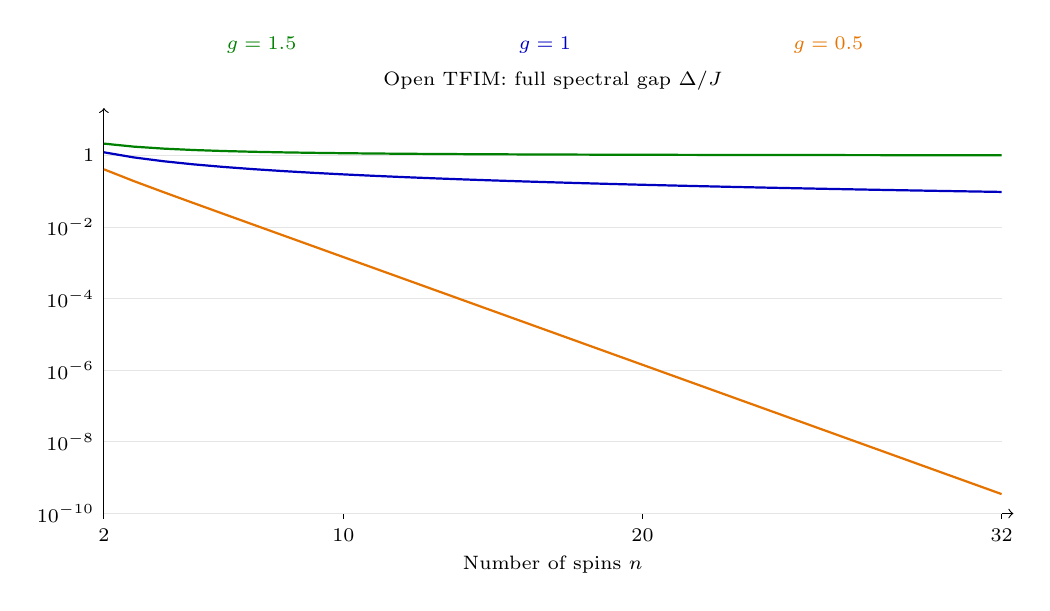
\begin{tikzpicture}[x=1cm,y=1cm,font=\scriptsize]
\draw[->] (0.0000,0.0000)--(11.5500,0.0000);
\draw[->] (0.0000,0.0000)--(0.0000,5.1500);
\draw (0.0000,0.0000)--+(0,-.07) node[below] {$2$};
\draw (3.0400,0.0000)--+(0,-.07) node[below] {$10$};
\draw (6.8400,0.0000)--+(0,-.07) node[below] {$20$};
\draw (11.4000,0.0000)--+(0,-.07) node[below] {$32$};
\draw[gray!20] (0.0000,0.0000)--+(11.4000,0);
\node[left] at (0.0000,0.0000) {$10^{-10}$};
\draw[gray!20] (0.0000,0.9091)--+(11.4000,0);
\node[left] at (0.0000,0.9091) {$10^{-8}$};
\draw[gray!20] (0.0000,1.8182)--+(11.4000,0);
\node[left] at (0.0000,1.8182) {$10^{-6}$};
\draw[gray!20] (0.0000,2.7273)--+(11.4000,0);
\node[left] at (0.0000,2.7273) {$10^{-4}$};
\draw[gray!20] (0.0000,3.6364)--+(11.4000,0);
\node[left] at (0.0000,3.6364) {$10^{-2}$};
\draw[gray!20] (0.0000,4.5455)--+(11.4000,0);
\node[left] at (0.0000,4.5455) {$1$};
\node at (5.7000,-0.6500) {\lr{Number of spins} $n$};
\node at (5.7000,5.5000) {\lr{Open TFIM: full spectral gap} $\Delta/J$};
\draw[green!50!black,thick,] plot coordinates {(0.00000,4.69769) (0.38000,4.65924) (0.76000,4.63405) (1.14000,4.61647) (1.52000,4.60366) (1.90000,4.59402) (2.28000,4.58657) (2.66000,4.58069) (3.04000,4.57598) (3.42000,4.57214) (3.80000,4.56898) (4.18000,4.56634) (4.56000,4.56411) (4.94000,4.56222) (5.32000,4.56060) (5.70000,4.55920) (6.08000,4.55799) (6.46000,4.55692) (6.84000,4.55599) (7.22000,4.55516) (7.60000,4.55443) (7.98000,4.55378) (8.36000,4.55319) (8.74000,4.55266) (9.12000,4.55219) (9.50000,4.55176) (9.88000,4.55137) (10.26000,4.55102) (10.64000,4.55069) (11.02000,4.55039) (11.40000,4.55012)};
\node[text=green!50!black] at (2.00,5.95) {$g=1.5$};
\draw[blue!75!black,thick,] plot coordinates {(0.00000,4.58729) (0.38000,4.52247) (0.76000,4.47351) (1.14000,4.43423) (1.52000,4.40145) (1.90000,4.37332) (2.28000,4.34869) (2.66000,4.32679) (3.04000,4.30707) (3.42000,4.28914) (3.80000,4.27271) (4.18000,4.25753) (4.56000,4.24344) (4.94000,4.23029) (5.32000,4.21796) (5.70000,4.20635) (6.08000,4.19539) (6.46000,4.18500) (6.84000,4.17513) (7.22000,4.16573) (7.60000,4.15676) (7.98000,4.14818) (8.36000,4.13996) (8.74000,4.13206) (9.12000,4.12447) (9.50000,4.11716) (9.88000,4.11011) (10.26000,4.10331) (10.64000,4.09673) (11.02000,4.09036) (11.40000,4.08419)};
\node[text=blue!75!black] at (5.60,5.95) {$g=1$};
\draw[orange!90!black,thick,] plot coordinates {(0.00000,4.37147) (0.38000,4.22166) (0.76000,4.08034) (1.14000,3.94202) (1.52000,3.80471) (1.90000,3.66773) (2.28000,3.53086) (2.66000,3.39401) (3.04000,3.25718) (3.42000,3.12035) (3.80000,2.98351) (4.18000,2.84668) (4.56000,2.70985) (4.94000,2.57302) (5.32000,2.43619) (5.70000,2.29936) (6.08000,2.16252) (6.46000,2.02569) (6.84000,1.88886) (7.22000,1.75203) (7.60000,1.61520) (7.98000,1.47836) (8.36000,1.34153) (8.74000,1.20470) (9.12000,1.06787) (9.50000,0.93104) (9.88000,0.79421) (10.26000,0.65737) (10.64000,0.52054) (11.02000,0.38371) (11.40000,0.24688)};
\node[text=orange!90!black] at (9.20,5.95) {$g=0.5$};
\end{tikzpicture}
	\caption{گاف زنجیره باز از محاسبه مقادیر تکین برای $g=1.5,1,0.5$. منحنی فاز مرتب شکافت کل کم‌انرژی را نشان می‌دهد، نه گاف حجمی. قدرت محلی $J=1$ ثابت است.}
	\label{fig:gap-size-scaling}
\end{figure}

\subsection{هزینه یافتن گاف در برابر هزینه اجرا}
اگر $\|H'\|$ با $n$ رشد کند، تخمین زمان باید این رشد را هم لحاظ کند.
گاف چندجمله‌ای همراه مسیر هموارِ قابل‌ساخت و مشتقات کنترل‌شده با اجرای کارآمد سازگار است؛ اثبات کارایی به هزینه تمام اجزا نیاز دارد.

در بدترین حالت، تعیین انرژی پایه هامیلتونی محلی با دقت وعده‌داده‌شده معکوس چندجمله‌ای، \lr{QMA}-کامل است؛ \lr{QMA} همتای کوانتومی بررسی گواه محاسباتی است.
این نتیجه اثبات سختی هر نمونه فیزیکی یا طبقه‌بندی یکسان همه مسائل گاف نیست~\cite{GapGharibian2015}.
حل‌ناپذیری تصمیم‌گیری گاف در حد ترمودینامیکی برای خانواده‌های خاص نتیجه دیگری است و مانع قطری‌سازی ماتریس متناهی معلوم نمی‌شود~\cite{GapCubitt2015}.

برازش چند اندازه کوچک به نمایی یا توانی کافی نیست. داده بزرگ‌تر، تقارن، مرزها و مدل برازش جایگزین را بررسی کنید.
در مسائل بی‌نظم علاوه بر میانگین، توزیع $\log\Delta_{\min}$ و نمونه‌های نادر اهمیت دارند.

\section{کاهش زمان و بهای آن}
\label{sec:gap-control}
\begin{enumerate}
	\item \textbf{زمان‌بندی و هموارکردن ابتدا/انتها.}
	سرعت را با گاف و عناصر گذار تنظیم کنید؛ هزینه برآورد مسیر جدا حساب شود.
	\item \textbf{تغییر مسیر.}
	جمله قابل‌کنترل $f(s)H_{\mathrm{cat}}$ با $f(0)=f(1)=0$ اضافه کنید.
	کل مسیر جدید باید بررسی شود؛ بزرگ‌شدن گاف در یک نقطه کافی نیست.
	افزایش دامنه یا غیرمحلی‌شدن جمله‌ها منابع اضافی‌اند.
	\item \textbf{رانش جبران‌کننده گذار.}
	در قرارداد
	\begin{equation}
		H_{\mathrm{tot}}=H+\dot s\,{\cal A}_s,\qquad
		\langle m|{\cal A}_s|n\rangle
		=i\hbar\frac{\langle m|H'|n\rangle}{E_n-E_m}\quad(m\ne n),
	\end{equation}
	جمله اضافی گذار ناشی از حرکت پایه را جبران می‌کند. نزدیک گاف کوچک می‌تواند بزرگ یا غیرمحلی شود.
	روش وردشی \lr{Sels--Polkovnikov} با محدودکردن $\mathcal{A}_s$ به عملگرهای قابل‌اجرا، تقریب عملی‌تری می‌سازد؛ بهبود وابسته به مدل و منابع کنترل است~\cite{GapSels2017}.
	\item \textbf{مسیر غیرآدیاباتیک و وردشی.}
	\lr{QAOA} یا کنترل بهینه می‌تواند عمداً در میانه حالت برانگیخته را اشغال کند.
	معیار، موفقیت در هزینه کل برابر است؛ چنین پروتکلی صرفاً آزمون قضیه آدیاباتیک نیست.
\end{enumerate}
در سامانه باز، اجرای طولانی‌تر ممکن است ناهمدوسی را بیشتر کند.
مقایسه $k_BT_{\mathrm{bath}}$ با گاف مفید است، اما نرخ گذار و عملگر جفت‌شدگی محیط هم مهم‌اند.
گاف لیوویلی معادله مادر با گاف انرژی هامیلتونی یکسان نیست.

\section{مرور هدفمند منابع و روش‌های جاری}
\label{sec:gap-papers}
این مرور گزینشی بر منابع بررسی‌شده تا ۱۴ سپتامبر ۲۰۲۶ تکیه دارد؛ مرور نظام‌مند همه مقالات نیست.
برای پوشش نظریه، محاسبه و آزمایش، چند مسیر مکمل انتخاب شده‌اند.
وضعیت پیش‌چاپ از مقاله منتشرشده جدا شده است.

\paragraph{پایه نظری و محاسبات کلاسیک.}
\lr{Jansen--Ruskai--Seiler (2007)} برای فرض‌ها و کران آدیاباتیک،
\lr{Roland--Cerf (2002)} برای زمان‌بندی محلی،
و مرور \lr{Schollwock (2011)} برای \lr{MPS/DMRG} مراجع آغاز مناسب‌اند.
مرور \lr{Albash--Lidar (2018)} پیوند این مباحث با محاسبه آدیاباتیک را توضیح می‌دهد~\cite{GapJansen2007,GapRoland2002,GapSchollwock2011,AlbashLidar2018}.

\paragraph{برآورد ترکیبی گاف با پردازش سیگنال؛ مقاله ۲۰۲۵.}
\lr{Lee, Myers, Scarola} در \lr{Physical Review A 111, 022421}
تحول کوانتومی، بهینه‌سازی حالت آزمایشی و پردازش کلاسیک سیگنال را ترکیب می‌کنند.
تحلیل مقاومت به نویز برای مدل‌های مشخص انجام شده؛ این به معنای حذف همه نویزها نیست.
کاربرد برای پروژه ما: بررسی قابل‌دیدن بودن قله گاف و هزینه شات/عمق در امتداد مسیر، همراه آزمون حساسیت به مدل نویز~\cite{GapLee2025}.

\paragraph{آماده‌سازی آدیاباتیک و برازش نوسان؛ پیش‌چاپ دسامبر ۲۰۲۵.}
\lr{Cugini et al.} در
\lr{Spectral Gap Estimation via Adiabatic Preparation}
از برهم‌نهی دو حالت و نوسان مشاهده‌پذیر استفاده می‌کنند؛ نتایجی برای آیزینگ و مدل‌های مولکولی و اجرای آیزینگ تا ۲۰ کیوبیت گزارش شده است.
برای انتقال ایده به پروژه، باید نشان داد دو شاخه مطلوب آماده شده‌اند، مشاهده‌پذیر وزن گذار دارد و برازش چندقله‌ای لازم نیست.
هزینه آماده‌سازی را نمی‌توان هنگام ادعای کاهش هزینه اندازه‌گیری گاف حذف کرد~\cite{GapCugini2025}.

\paragraph{شمارش طیفی؛ مقاله منتشرشده ۲۰۲۶.}
\lr{Carrera Vazquez--Sobczyk} در \lr{Quantum 10, 2067}
گاف مرتب‌شده ماتریس هرمیتی و نقطه میانی آن را با پرسمان شمارش بررسی می‌کنند.
در مدل دسترسی \lr{QRAM}، هزینه شامل عامل
$D^2/(\epsilon^2\Delta_k^2)$ و عوامل چندلگاریتمی است؛ $\epsilon$ دقت نسبی گاف در قرارداد نرمال‌سازی مقاله است.
با $D=2^n$ این عامل هنوز نمایی در تعداد کیوبیت سامانه است؛ تعداد کیوبیت لگاریتمی را نباید با زمان چندجمله‌ای در $n$ یکی گرفت.
سهم پژوهشی آن الگوریتم و تحلیل در مدل دسترسی مشخص است~\cite{GapCarrera2026}.

\paragraph{زیرفضای نمونه‌برداری‌شده؛ مسیر مرتبط، نه تضمین آماده گاف.}
\lr{Yu et al. (2025)} در \lr{SKQD} نمونه‌برداری کوانتومی از حالت‌های کریلوف را با قطری‌سازی کلاسیک ترکیب می‌کنند.
تضمین همگرایی پایه فرض‌هایی از جمله ساختار حالت و پراکندگی آن در پایه نمونه‌برداری دارد.
تعمیم به گاف مستلزم حضور و کنترل خطای حالت برانگیخته نیز هست؛ این یک فرصت پژوهشی است، نه نتیجه خودکارِ روش پایه~\cite{GapYu2025}.
\lr{VQD} مرجع دیگری برای هدف‌گیری ترازهای برانگیخته است~\cite{GapHiggott2019}.

\section{جریان کاری و مسیرهای پیشنهادی پژوهش}
\label{sec:gap-projects}
\begin{figure}[htbp]
	\centering
\begin{tikzpicture}[node distance=7mm,>=Latex,
 every node/.style={font=\small},
 gapbox/.style={draw,rounded corners,align=center,text width=10.6cm,minimum height=10mm,fill=blue!5}]
\node[gapbox] (a) {\RL{مدل، واحد انرژی، اندازه، تقارن و تعریف گاف}};
\node[gapbox,below=of a] (b) {\RL{محاسبهٔ چند تراز یا طیف‌سنجی با مشاهده‌پذیر مناسب}};
\node[gapbox,below=of b] (c) {\RL{کنترل خطا و جست‌وجوی تطبیقی کمینه در مسیر}};
\node[gapbox,below=of c] (d) {\RL{طراحی زمان‌بندی با گاف و عناصر ماتریسی گذار}};
\node[gapbox,below=of d] (e) {\RL{آزمون موفقیت و منابع؛ مقایسه در اندازه‌های مختلف}};
\draw[->] (a)--(b);
\draw[->] (b)--(c);
\draw[->] (c)--(d);
\draw[->] (d)--(e);
\draw[->] (e.east)--++(.65,0)|-(c.east);
\end{tikzpicture}

	\caption{گاف، عدم‌قطعیت و هزینه یافتن آن، همگی ورودی طراحی زمان‌بندی‌اند؛ حلقه با آزمون دینامیکی بسته می‌شود.}
	\label{fig:gap-workflow}
\end{figure}
برای هر نتیجه ثبت کنید: مدل و واحد انرژی، اندازه و مرزها، تعریف گاف و بخش تقارنی، روش، خطای ترازها، دقت شبکه $s$، محل کمینه، عناصر گذار، زمان کل، احتمال موفقیت و منابع کلاسیک/کوانتومی.

سه موضوع قابل‌آغاز با فرضیه قابل‌آزمون:
\begin{enumerate}
	\item \textbf{زمان‌بندی مقاوم به خطای گاف در زنجیره آیزینگ.}
	مرجع دقیق برای اندازه‌های کوچک؛ سپس برآورد نویزی و مقایسه جاروب خطی، محلی و محافظه‌کارانه در زمان برابر.
	معیار: احتمال موفقیت، بدترین افت تحت خطای گاف و هزینه نمونه‌برداری.
	نوآوری باید در تحمل عدم‌قطعیت یا کاهش هزینه باشد، نه صرف بازتولید زمان‌بندی محلی.
	\item \textbf{طیف‌سنجی با انتخاب مشاهده‌پذیر بر اساس تقارن.}
	چند عملگر با قواعد انتخاب متفاوت را مقایسه کنید و بسنجید چه وقت اولین قله، گاف هدف را پنهان می‌کند.
	مرجع قطری‌سازی، برازش چندفرکانسی و نویز خوانش لازم‌اند؛ مقالات \lr{Lee} و \lr{Cugini} نقطه شروع‌اند.
	\item \textbf{زیرفضای مشترک پایه و برانگیخته.}
	در \lr{VQD/Krylov} خطای دو تراز و اندازه زیرفضا را کنترل و با مرجع مقایسه کنید.
	سؤال: آیا در هزینه یکسان، هدف‌گیری هم‌زمان دو حالت از تفاضل دو بهینه‌سازی مستقل قابل‌اعتمادتر است؟
\end{enumerate}
این‌ها پیشنهاد مسئله‌اند، نه ادعای نوآوری اثبات‌شده. انتخاب نهایی پس از تعیین مدل، سکو، دامنه اندازه‌ها و بررسی دقیق‌تر پیشینه انجام می‌شود. چارچوب گسترده‌تر برآورد و مهندسی گاف، با سه طرح مقاله، در فصل~\ref{chap:gap-energy} آمده است.
فایل \lr{figures/gap\_research\_compute.py} محاسبات و نمودارهای این بخش را بازتولید می‌کند؛ داده‌ها و آزمون همگرایی کنار شکل‌ها ذخیره می‌شوند.
دو اسپین برای فهم و راستی‌آزمایی است و به‌تنهایی شاهد مزیت کوانتومی نیست.
\endgroup
% END GAP RESEARCH EXPANSION


\section{ارتباط}

دو پرسش در فصل~\ref{chap:dyn-spec}، ابزار دیجیتال در فصل~\ref{chap:digital-tools}، \lr{QPE} از تحول تغذیه می‌کند و \lr{VQE} رهیافت سومی است (وردشی) در فصل~\ref{chap:spectral-tools}، و آنالوگ در فصل~\ref{chap:hardware} آمده است. مدل‌های اسپینی در فصل~\ref{chap:models} آمده‌اند. پیاده‌سازی \lr{Qiskit}یِ مثال دوکیوبیتی در بخش~\ref{sec:adi-ising-qiskit} است. مقیاس‌بندی $n\to\Delta_{\min}(n)\to T(n)$ در بخش~\ref{sec:complexity-scaling} و جزئیات \lr{TFIM}/\lr{QMA} در بخش~\ref{sec:gap-scaling} است. برآورد گاف، مهندسی مسیر، و طرح مقاله در فصل~\ref{chap:gap-energy} است.

\section{چه وقت استفاده می‌شود}

تحول: دینامیک، پاسخ زمانی، quench، و هر الگوریتمی که $f(H)$ یا $U(t)$ می‌خواهد (بخش‌های~\ref{sec:time-evolution} و~\ref{sec:evo-example}). آدیاباتیک: آماده‌سازی حالت پایه وقتی گاف مسیر کنترل‌پذیر به نظر می‌رسد، وقتی مسئله به \lr{Ising}/بهینه‌سازی نگاشته می‌شود، یا وقتی سخت‌افزار به‌طور طبیعی یک $H(s)$ می‌دهد. اگر $\Delta_{\min}$ مسیر را نمی‌شناسید، اول همان را بسنجید؛ وگرنه $T$ حدسِ کور است. برای تمرین عددی روی همین مثال دوکیوبیتی، بخش~\ref{sec:adi-ising-qiskit} را با محیط \lr{qcomputing} اجرا کنید.

\begin{remark}[جای توسعه]
	برای تحول: $H(t)$ با انتگرال زمانی مرتب‌شده؛ توابع همبستگی چندزمانی. برای آدیاباتیک: زمان‌بندی تطبیقی با عدم‌قطعیت گاف؛ آزمون‌های نویزی و تعمیم به سامانه باز؛ عبور از نقطه بحرانی در حد ترمودینامیکی؛ تروترِ مرتبهٔ بالاتر و مقایسهٔ خطای مدار با مرجع شرودینگر در بخش~\ref{sec:adi-ising-qiskit}. برای مقیاس‌بندی: برازش $\Delta_{\min}(n)$ روی اندازه‌های بزرگ‌تر از چند نقطه و جدا کردن گاف حجمی از شکافت لبه‌ای. برای گسسته‌سازی وردشیِ مسیر آدیاباتیک: بخش~\ref{sec:qaoa} (\lr{QAOA}). برای تمرکز پژوهشی روی برآورد و مهندسی گاف در کل شبیه‌سازی کوانتومی: فصل~\ref{chap:gap-energy}.
\end{remark}